\documentclass[%
%%% PARA ESCOLHER O ESTILO TIRE O SIMBOLO %(COMENTÁRIO)
%SemVinculoColorido,
%SemFormatacaoCapitulo,
%SemFolhaAprovacao,
%SemImagens,
%CitacaoNumerica, %% o padrão é citação tipo autor-data
%PublicacaoDissOuTese, %% (é também o "default") com ficha catal. e folha de aprovação em branco. Caso tenha lista de símbolos e lista de siglas e abreviaturas retirar os comentários dos arquivos siglas.tex e abreviaturasesiglas.tex. Retirar também os comentários indicados nesse arquivo, nos includes
%PublicacaoArtigoOuRelatorio, %% texto sequencial, sem quebra de páginas nem folhas em branco
%PublicacaoProposta, %% igual tese/dissertação, mas sem ficha catal. e fol. de aprov.
%PublicacaoLivro, %% com capítulos
%PublicacaoLivro,SemFormatacaoCapitulo, %% sem capítulos
%english,portuguese %% para os documentos em Português com abstract.tex em Inglês
portuguese,english %% para os documentos em Inglês com abstract.tex em Português
,LogoINPE % comentar essa linha para fazer aparecer o logo do Governo
,CCBY % as opções de licença são: CCBY, CCBYSA, CCBYND, CCBYNC, CCBYNCSA, CCBYNCND, GPLv3 e INPECopyright
]{tdiinpe220101}
%]{../../../../../iconet.com.br/banon/2008/03.25.01.19/doc/tdiinpe}

% PARA EXIBIR EM ARIAL TIRAR O COMENTÁRIO DAS DUAS LINHAS SEGUINTES
%\renewcommand{\rmdefault}{phv} % Arial
%\renewcommand{\sfdefault}{phv} % Arial

% PARA PUBLICAÇÕES EM INGLÊS:
% renomear o arquivo: abnt-alf.bst para abnt-alfportuguese.bst
% renomear o arquivo: abnt-alfenglish.bst para abnt-alf.bst

% LATEX FONT SIZES
% command           10pt    11pt    12pt
% \tiny             5       6       6
% \scriptsize       7       8       8
% \footnotesize     8       9       10
% \small            9       10      10.95
% \normalsize       10      10.95   12
% \large            12      12      14.4
% \Large            14.4    14.4    17.28
% \LARGE            17.28   17.28   20.74
% \huge             20.74   20.74   24.88
% \Huge             24.88   24.88   24.88

% FLOAT: h=here, t=top, b=bottom, p=(page of floats)
% ex.: \begin{figure}[ht]

%%% Pacotes já previamente carregados: 
%%% ifthen,calc,graphicx,color,inputenc,babel,hyphenat,array,setspace,bigdelim,multirow,supertabular,tabularx,longtable,lastpage,lscape,rotate,caption2,amsmath,amssymb,amsthm,subfigure,tocloft,makeidx,eso-pic,calligra,hyperref,ae,fontenc
%%% insira neste campo, comandos de LaTeX %%%
%%% \usepackage{_exemplo_}
%\watermark{Revisão No. ##} %% use o comando \watermark para identificar a versão de seu documento
%% comente este comando quando for gerar a versão final
%\usepackage{rotating}	% rotating of text and tables
%\usepackage{dsfont}	% Math symbols
%\usepackage{comment}
%\usepackage{lipsum}     % to check formatting
%\usepackage{afterpage}  % \afterpage{\clearpage}
%----------------------------------------
\usepackage{microtype}  % better text justification
\usepackage{booktabs}   % enhances the quality of tables
%----------------------------------------
\usepackage{listings}
%\renewcommand{\lstlistingname}{Listagem}
\lstdefinestyle{mystyle}{
%backgroundcolor=\color{backcolour},
commentstyle=   \color{codegray},
keywordstyle=[1]\color{islamicgreen}\bfseries,
keywordstyle=[2]\color{patriarch},
keywordstyle=[3]\color{red-brown},
identifierstyle=\color{richelectricblue},
stringstyle=    \color{red-violet},
numberstyle=\tiny\color{codegray},% line numbering
basicstyle          = \ttfamily\footnotesize,
frame               = single,
rulecolor			= \color{codegray},
columns             = fullflexible,
breakatwhitespace   = false,
breaklines          = true,
keepspaces          = true,
showspaces          = false,
showstringspaces    = false,
inputencoding       = utf8,
extendedchars       = true,
literate            =
{á}{{\'a}}1 {é}{{\'e}}1 {í}{{\'i}}1 {ó}{{\'o}}1 {ú}{{\'u}}1
{Á}{{\'A}}1 {É}{{\'E}}1 {Í}{{\'I}}1 {Ó}{{\'O}}1 {Ú}{{\'U}}1
{à}{{\`a}}1 {è}{{\`e}}1 {ì}{{\`i}}1 {ò}{{\`o}}1 {ù}{{\`u}}1
{À}{{\`A}}1 {È}{{\'E}}1 {Ì}{{\`I}}1 {Ò}{{\`O}}1 {Ù}{{\`U}}1
{ä}{{\"a}}1 {ë}{{\"e}}1 {ï}{{\"i}}1 {ö}{{\"o}}1 {ü}{{\"u}}1
{Ä}{{\"A}}1 {Ë}{{\"E}}1 {Ï}{{\"I}}1 {Ö}{{\"O}}1 {Ü}{{\"U}}1
{â}{{\^a}}1 {ê}{{\^e}}1 {î}{{\^i}}1 {ô}{{\^o}}1 {û}{{\^u}}1
{Â}{{\^A}}1 {Ê}{{\^E}}1 {Î}{{\^I}}1 {Ô}{{\^O}}1 {Û}{{\^U}}1
{œ}{{\oe}}1 {Œ}{{\OE}}1 {æ}{{\ae}}1 {Æ}{{\AE}}1 {ß}{{\ss}}1
{ç}{{\c c}}1 {Ç}{{\c C}}1 {ø}{{\o}}1 {å}{{\r a}}1 {Å}{{\r A}}1
{€}{{\EUR}}1 {£}{{\pounds}}1 {ã}{{\~a}}1 {Ã}{{\~A}}1,
showtabs=false,
tabsize=2,
numbers=left,
numbersep=5pt,
aboveskip=2pt,
belowskip=9pt,
belowcaptionskip=\bigskipamount,
% captionpos=b,
}
\lstset{}
\lstset{style=mystyle}
%----------------------------------------
\graphicspath{{img/}}
\pdfstringdefDisableCommands{ \def\\{} }% evita erro token not allowed in a PDF
%----------------------------------------
\definecolor{blue}{RGB}{66, 133, 244}% #4285f4
\definecolor{red}{RGB}{234, 67, 53}% #ea4335
\definecolor{orange}{RGB}{251, 188, 4}% #fbbc04
\definecolor{darkorange}{RGB}{255, 109, 1}% #ff6d01
\definecolor{green}{RGB}{52, 168, 83}% #34a853
\definecolor{tropicalrainforest}{rgb}{0.0, 0.46, 0.37}% tropicalrainforest
\definecolor{cyan}{RGB}{70, 189, 198}% #46bdc6
\definecolor{gray}{gray}{.50}
\definecolor{islamicgreen}{rgb}{0.0, 0.56, 0.0}
\definecolor{light-gray}{gray}{.85}
\definecolor{codegray}{gray}{0.5}
\definecolor{richelectricblue}{rgb}{0.03, 0.57, 0.82}
\definecolor{violet}{RGB}{238, 130, 238}
\definecolor{red-violet}{rgb}{0.78, 0.08, 0.52}
\definecolor{patriarch}{rgb}{0.5, 0.0, 0.5}
\definecolor{red-brown}{rgb}{0.65, 0.16, 0.16}
\definecolor{backcolour}{rgb}{0.97, 0.97, 0.97}
\definecolor{alt}{rgb}{0.78, 0.08, 0.52}% red-violet
\newcommand{\ALT}[1]{{\color{alt}#1}}
%----------------------------------------
%\definecolor{olive}{rgb}{0.5, 0.5, 0.0}% olive
%\definecolor{green}{rgb}{0.0, 0.46, 0.37}
%\definecolor{alt}{rgb}{0.66,0.66,0.66}% #A9A9A9
%\definecolor{alt}{rgb}{0.0, 0.5, 0.0}%
%\definecolor{armygreen}{rgb}{0.29, 0.33, 0.13}% armygreen
%\definecolor{britishracinggreen}{rgb}{0.0, 0.26, 0.15}% britishracinggreen
%\definecolor{darkgreen}{rgb}{0.0, 0.2, 0.13}% darkgreen
%\definecolor{darkjunglegreen}{rgb}{0.1, 0.14, 0.13}% darkjunglegreen
%----------------------------------------
\newcommand{\fcred}[1]{\textbf{\color{red}#1}}
\newcommand{\fcgreen}[1]{\textbf{\color{green}#1}}
\newcommand{\fcblue}[1]{\textbf{\color{blue}#1}}
\newcommand{\fcorange}[1]{\textbf{\color{orange}#1}}
\newcommand{\fcdarkorange}[1]{\textbf{\color{darkorange}#1}}
\newcommand{\fccyan}[1]{\textbf{\color{cyan}#1}}
\newcommand{\fcgray}[1]{\textbf{\color{gray}#1}}
%----------------------------------------
\newcommand{\no}[0]{\textsuperscript{\b{o}}}

% Makes tables and figures the same type of float, so that they are placed in the same queue, and hence appear in the order of appearance. http://tex.stackexchange.com/questions/127742/place-floating-tables-and-figures-in-order-of-appearance
\makeatletter
\let\ftype@table\ftype@figure
\makeatother

\newcommand{\TABLE}[4][6pt]{%
\begin{table}[!hbt]%
%\vspace{4mm}
\caption{#2}%
\begin{center}%
\footnotesize%
\setlength{\tabcolsep}{#1}%
\input{tab/#4}%
\end{center}%
\legenda{}%
\vspace{-1mm}%
\FONTE{#3}%
\label{#4}%
\vspace{-4mm}%
\end{table}%
}

\newcommand{\FIGURE}[1][.95]{%
\def\ArgI{#1}%
\FIGURERELAY}
\newcommand{\FIGURERELAY}[4][-2mm]{%
\begin{figure}%
\vspace{-3mm}%
\caption{#2}%
\vspace{2mm}%
\centering%
\includegraphics[width=\ArgI\linewidth]{#4}%
\legenda{}%
\vspace{#1}%
\FONTE{#3}%
\label{#4}%
\vspace{-4mm}%
\end{figure}%
}

% = capital autoref =
% http://tex.stackexchange.com/questions/446748/how-to-redefine-section-and-subsection-in-autoref-names
\addto\extrasenglish{%
\renewcommand\chapterautorefname{Chapter}%
\renewcommand\sectionautorefname{Section}%
\renewcommand\subsectionautorefname{Subsection}%
\renewcommand\subsubsectionautorefname{Subsubsection}%
}

%   ____                    
%  / ___|_____   _____ _ __ 
% | |   / _ \ \ / / _ \ '__|
% | |__| (_) \ V /  __/ |   
%  \____\___/ \_/ \___|_|  
%%%%%%%%%%%%%%%%%%%%%%%%%%%%%%%%%%%%%%%%%%%%%%%%%%%%%%
%\serieinpe{INPE-NNNNN-TDI/NNNN} %% não mais usado
%%%%%%%%%%%%%%%%%%%%%%%%%%%%%%%%%%%%%%%%%%%%%%%%%%%%%%

\titulo{Common MPI-Based HPC Approaches in Python Evaluated for Selected Test Cases}
\title{Soluções Comuns Baseadas em MPI para Processamento de Alto Desempenho em Python Avaliadas em Casos de Teste Selecionados} %% 
\author{xxxx} %% coloque o nome do(s) autor(es)
\descriccao{Master's Dissertation of the Graduate Course in Applied Computing, guided by Dr. xxxx, approved in MMMM DD, AAAA.}


%--ABAIXO NÃO PREENCHE--------------------------------------

\repositorio{aa/bb/cc/dd} %% repositório onde está depositado este documento - na omissão, será preenchido pelo SID
\tipoDaPublicacao{TDI}	%% tipo da publicação (NTC, RPQ, PRP, MAN, PUD, TDI, TAE e PRE) na ausência do número de série INPE, caso contrário deixar vazio
\IBI{xx/yy} %% IBI (exemplo: J8LNKAN8PW/36CT2G2) quando existir, caso contrário o nome do repositório onde está depositado o documento

\date{AAAA}%ano da publicação

%%%%%%%%VERSO DA CAPA%%%%%%%%%%%%%%%%%%%%%%%%%%%%%%

\tituloverso{\vspace{-0.9cm}\textbf{\PublicadoPor:}}
\descriccaoverso{Instituto Nacional de Pesquisas Espaciais - INPE\\
Gabinete do Diretor (GB)\\
Serviço de Informação e Documentação (SID)\\
Caixa Postal 515 - CEP 12.245-970\\
São José dos Campos - SP - Brasil\\
Tel.:(012) 3945-6923/6921\\
Fax: (012) 3945-6919\\
E-mail: {\url{pubtc@sid.inpe.br}}
}

\descriccaoversoA{\textbf{\ConselhoDeEditoracao:}\\
\textbf{\Presidente:}\\
Marciana Leite Ribeiro - Serviço de Informação e Documentação (SID)\\
\textbf{\Membros:}\\
Dr. Gerald Jean Francis Banon - Coordenação Observação da Terra (OBT)\\
Dr. Amauri Silva Montes - Coordenação Engenharia e Tecnologia Espaciais (ETE)\\
Dr. André de Castro Milone - Coordenação Ciências Espaciais e Atmosféricas (CEA)\\
Dr. Joaquim José Barroso de Castro -  Centro de Tecnologias Espaciais (CTE)\\
Dr. Manoel Alonso Gan - Centro de Previsão de Tempo e Estudos Climáticos (CPT)\\
Drª Maria do Carmo de Andrade Nono - Conselho de Pós-Graduação\\
Dr. Plínio Carlos Alvalá - Centro de Ciência do Sistema Terrestre (CST)\\
\textbf{\BibliotecaDigital:}\\
Dr. Gerald Jean Francis Banon - Coordenação de Observação da Terra (OBT)\\
Clayton Martins Pereira - Serviço de Informação e Documentação (SID)\\
%Jefferson Andrade Ancelmo - Serviço de Informação e Documentação (SID)\\
%Simone A. Del-Ducca Barbedo - Serviço de Informação e Documentação (SID)\\
%Deicy Farabello - Centro de Previsão de Tempo  e Estudos Climáticos (CPT)\\
\textbf{\RevisaoNormalizacaoDocumentaria:}\\
Simone Angélica Del Ducca Barbedo - Serviço de Informação e Documentação (SID) \\
%Marilúcia Santos Melo Cid - Serviço de Informação e Documentação (SID)\\
Yolanda Ribeiro da Silva Souza - Serviço de Informação e Documentação (SID)\\
\textbf{\EditoracaoEletronica:}\\
Marcelo de Castro Pazos - Serviço de Informação e Documentação (SID)\\
André Luis Dias Fernandes - Serviço de Informação e Documentação (SID)\\
}

%%%%%%%%%%%%%%%%%%%FOLHA DE ROSTO

%%%%%%%%%%%%%%%FICHA CATALOGRÁFICA
%% NÃO PREENCHER - SERÁ PREENCHIDO PELO SID

\cutterFICHAC{Cutter}
\autorUltimoNomeFICHAC{Sobrenome, Nomes} %% exemplo: Fuckner, Marcus André
\autorFICHAC {Nome Completo do Autor1; Nome Completo do Autor2} %% Campo opcional (se não usado prevalece \author)
\tituloFICHAC{Titulo da publicação}
\instituicaosigla{INPE}
\instituicaocidade{São José dos Campos}
\paginasFICHAC{\pageref{numeroDePáginasDoPretexto} + \pageref{LastPage}} %% número total de páginas
%\serieinpe{INPE-00000-TDI/0000} %% não mais usado
\palavraschaveFICHAC{1.~Palavra chave. 2.~Palavra chave 3.~Palavra chave. 4.~Palavra chave. 5.~Palavra chave  I.~\mbox{Título}.} %% recomenda-se pelo menos 5 palavras-chaves - \mbox{} é para evitar hifenização 
\numeroCDUFICHAC{000.000} %% número do CDU 

% Nota da ficha (para TD)
\tipoTD{Dissertação ou Tese} % Dissertação ou Tese
\cursoFA{Mestrado ou Doutorado em Nome do Curso}
\instituicaoDefesa{Instituto Nacional de Pesquisas Espaciais}
\anoDefesa{AAAA} % ano de defesa 
\nomeAtributoOrientadorFICHAC{Orientador}	% pode ser: Orientador, Orientadora ou Orientadores
\valorAtributoOrientadorFICHAC{José da Silva} % nome(s) completo(s)

%%%%%%%%%%%%%%%FOLHA DE APROVAÇAO PELA BANCA EXAMINADORA
\tituloFA{\textbf{ATENÇÃO! A FOLHA DE APROVAÇÃO SERÁ INCLUIDA POSTERIORMENTE.}}
%\cursoFA{\textbf{}}https://www.overleaf.com/project/60ba47037849dde4ef37e19e
\candidatoOUcandidataFA{}
\dataAprovacaoFA{}
\membroA{}{}{}
\membroB{}{}{}
\membroC{}{}{}
\membroD{}{}{}
\membroE{}{}{}
\membroF{}{}{}
\membroG{}{}{}
\ifpdf

 %% faça as modificações pertinentes no arquivo configuracao.tex

%\makeindex  %% gera INDEX, caso haja algum termo indexado no texto

\begin{document} %% início do documento %% não mexer

\sloppy	% forces overflowing words to move to the next line
%\marcaRegistrada{}	% comando opcional usado para informar abaixo da ficha catalográfica sobre marca registrada
\marcaRegistrada{Informar aqui sobre marca registrada (a modificação desta linha deve ser feita no arquivo publicacao.tex).}
%\financiamento{}	% comando opcional usado para informar abaixo da ficha catalográfica sobre fontes financiadoras
%\financiamento{Informar aqui sobre fontes financiadoras (a modificação desta linha deve ser feita no arquivo publicacao.tex).}
%\financiamento{O presente trabalho foi realizado com apoio da Coordenação de Aperfeiçoamento de Pessoal de Nível Superior - Brasil (CAPES) - Código de Financiamento 001.}
%\financiamento{This study was financed in part by the Coordenação de Aperfeiçoamento de Pessoal de Nível Superior - Brasil (CAPES) - Finance Code 001.}
\hypersetup{pageanchor=false} % evita problemas com nro. de p.
\maketitle % não alterar, gera páginas obrigatórias (folha de rosto, ficha catalográfica e folha de aprovação)
\hypersetup{pageanchor=true}
% Comente as linhas opcionais abaixo caso não as deseje
% \include{./docs/epigrafe}% Opcional
%\include{./docs/dedicatoria}% Opcional

%     _        _                        _          _                            _       
%   / \   ___| | ___ __   _____      _| | ___  __| | __ _ _ __ ___   ___ _ __ | |_ ___ 
%   / _ \ / __| |/ / '_ \ / _ \ \ /\ / / |/ _ \/ _` |/ _` | '_ ` _ \ / _ \ '_ \| __/ __|
%  / ___ \ (__|   <| | | | (_) \ V  V /| |  __/ (_| | (_| | | | | | |  __/ | | | |_\__ \
% /_/   \_\___|_|\_\_| |_|\___/ \_/\_/ |_|\___|\__,_|\__, |_| |_| |_|\___|_| |_|\__|___/
%                                                   |___/    
%%%%%%%%%%%%%%%%%%%%%%%%%%%%%%%%%%%%%%%%%%%%%%%%%%%%%%
% AGRADECIMENTOS %% opcional
%%%%%%%%%%%%%%%%%%%%%%%%%%%%%%%%%%%%%%%%%%%%%%%%%%%%%%

\begin{agradecimentos}  %% insira abaixo seus agradecimentos

\hypertarget{estilo:agradecimentos}{} %% uso para este Guia

I would like to express my sincere gratitude to the National Institute for Space Research (INPE) and to its Applied Computing postgraduate course, which enabled my research. Also, I am grateful to my advisor, Stephan Stephany, for his guidance and encouragement, and to the LNCC (National Laboratory for Scientific Computing) for the 205341 AMPEMI 2020-I scholarship, which allowed access to the Santos Dumont supercomputer (SINAPAD node of the Brazilian HPC system).

The current work was accomplished with the support of the Coordination for the Improvement of Higher Education Personnel, Brazil (CAPES - Coordenação de Aperfeiçoamento de Pessoal de Nível Superior, Brasil), Funding Code (Código de Financiamento) 001.

\end{agradecimentos}


 %% Opcional
%   _    _         _                  _   
%   / \  | |__  ___| |_ _ __ __ _  ___| |_ 
%   / _ \ | '_ \/ __| __| '__/ _` |/ __| __|
%  / ___ \| |_) \__ \ |_| | | (_| | (__| |_ 
% /_/   \_\_.__/|___/\__|_|  \__,_|\___|\__|
%%%%%%%%%%%%%%%%%%%%%%%%%%%%%%%%%%%%%%%%%%%%%%%%%%%%%%
% RESUMO %% obrigatório
%%%%%%%%%%%%%%%%%%%%%%%%%%%%%%%%%%%%%%%%%%%%%%%%%%%%%%

\begin{resumo}

%% neste arquivo resumo.tex
%% o texto do resumo e as palavras-chave têm que ser em Português para os documentos escritos em Português
%% o texto do resumo e as palavras-chave têm que ser em Inglês para os documentos escritos em Inglês
%% os nomes dos comandos \begin{resumo}, \end{resumo}, \palavraschave e \palavrachave não devem ser alterados

\hypertarget{estilo:resumo}{} %% uso para este Guia

A number of the most common MPI-based high-performance computing approaches available in the Python programming environment of the LNCC Santos Dumont supercomputer are compared using three selected test cases. Python includes specific libraries, development tools, implementations, documentation and optimization or parallelization resources. It provides a straightforward way to allow programs to be written with a high level of abstraction, but the parallelization features to exploit multiple cores, processors or accelerators such as GPUs are diverse and may not be easily selectable by the programmer. This work compares common approaches in Python to increase computing performance for three test cases: a 2D heat transfer problem solved by the finite difference method, a 3D fast Fourier transform applied to synthetic data, and asteroid classification using a random forest. The corresponding serial and parallel implementations in Fortran 90 were taken as references to compare the computational performance. In addition to the performance results, a discussion of the trade-off between easiness of programming and computational performance is included. This work is intended as a primer for using parallel HPC resources in Python.

\palavraschave{%
	\palavrachave{High performance computing}%
	\palavrachave{Python programming environment}%
	\palavrachave{Parallel computing}%
}
 
\end{resumo}
 %% obrigatório
%   _    _         _                  _   
%   / \  | |__  ___| |_ _ __ __ _  ___| |_ 
%   / _ \ | '_ \/ __| __| '__/ _` |/ __| __|
%  / ___ \| |_) \__ \ |_| | | (_| | (__| |_ 
% /_/   \_\_.__/|___/\__|_|  \__,_|\___|\__|
%%%%%%%%%%%%%%%%%%%%%%%%%%%%%%%%%%%%%%%%%%%%%%%%%%%%%%
% ABSTRACT
%%%%%%%%%%%%%%%%%%%%%%%%%%%%%%%%%%%%%%%%%%%%%%%%%%%%%%


\begin{abstract}

%% neste arquivo abstract.tex
%% o texto do resumo e as palavras-chave têm que ser em Inglês para os documentos escritos em Português
%% o texto do resumo e as palavras-chave têm que ser em Português para os documentos escritos em Inglês
%% os nomes dos comandos \begin{abstract}, \end{abstract}, \keywords e \palavrachave não devem ser alterados

%\selectlanguage{english}	%% para os documentos escritos em Português
\selectlanguage{portuguese}	%% para os documentos escritos em Inglês

\hypertarget{estilo:abstract}{} %% uso para este Guia


Algumas das abordagens de computação de alto desempenho mais comuns baseadas em MPI disponíveis no ambiente de programação Python do supercomputador LNCC Santos Dumont são comparadas usando três casos de teste selecionados. Python inclui bibliotecas específicas, ferramentas de desenvolvimento, implementações, documentação e recursos de otimização ou paralelização. Ele fornece uma maneira direta de permitir que programas sejam escritos com um alto nível de abstração, mas os recursos de paralelização para explorar vários núcleos, processadores ou aceleradores, como GPUs, são diversos e podem não ser facilmente selecionáveis pelo programador. Este trabalho compara abordagens comuns em Python para se obter processamento de alto desempenho desempenho utilizando três casos de teste: um problema de transmissão de calor bidimensional resolvido por diferenças finitas, uma transformada rápida de Fourier tridimensional aplicada a dados sintéticos e uma classificação de asteróides por floresta aleatória. As correspondentes implementações seriais e paralelas em Fortran 90 foram tomadas como referência para comparação de desempenho nesses casos de teste. Além dos resultados de desempenho, inclui-se uma discussão sobre o compromisso entre facilidade de programação e desempenho de processamento. Este trabalho pretende ser uma introdução para o uso de recursos de processamento de alto desempenho baseados em MPI para Python.


% ANTIGO:
% Algumas das soluções mais comuns baseadas em processamento de alto desempenho disponíveis no ambiente de programação Python e no supercomputador Santos Dumont do LNCC, foram comparadas utilizando três casos de teste selecionados. O ambiente Python inclui bibliotecas específicas, ferramentas de desenvolvimento, implementações prontas, documentação e recursos para otimização/paralelização de código. Provê uma maneira direta de programar num nível de abstração alto, mas recursos de paralelização para explorar múltiplos núcleos de processadores ou aceleradores como GPUs são diversos e podem não ser facilmente escolhidos pelo programador. Este trabalho compara abordagens comuns em Python para aumentar o desempenho de processamento. Três casos de teste são apresentados: método de diferenças finitas para resolver equações diferenciais parciais resultantes de equações de Poisson, método de transformada discreta de Fourier tridimensional, e método de floresta de decisão aleatória para aprendizado conjunto. As correspondentes implementações sequencial e paralela em Fortran 90 foram tomadas como referência, de modo a comparar seu desempenho com algumas implementações sequenciais e paralelas desses algoritmos. Além dos resultados de desempenho de processamento, foi incluída uma discussão sobre a solução de compromisso entre facilidade de programação versus desempenho de processamento. Teste trabalho tem a intenção de servir de guia introdutório para o uso de recursos de alto desempenho baseados em computação paralela no ambiente Python.




\keywords{%
	\palavrachave{Processamento de alto desempenho}%
	\palavrachave{Ambiente de programação Python}%
	\palavrachave{Computação paralela}%
}

%\selectlanguage{portuguese}    %% para os documentos escritos em Português
\selectlanguage{english}        %% para os documentos escritos em Inglês

\end{abstract}
 %% obrigatório
\includeListaFiguras %% obrigatório caso haja mais de 3 figuras, gerado automaticamente
\includeListaTabelas %% obrigatório caso haja mais de 3 tabelas, gerado automaticamente

%\include{./docs/abreviaturasesiglas} %% opcional. Altere o arquivo siglaseabreviaturas.tex
%\include{./docs/simbolos} %% opcional. Altere o arquivo simbolos.tex

\includeSumario     %% obrigatório, gerado automaticamente
\inicioIntroducao   %% não altere este comando
%% insira quantos capítulos desejar com o seguinte comando:
%\include{_pasta_do_arquivo_/_meu_arquivo_} %%sem a extensão
%% note que deverá haver um arquivo _meu_arquivo_.tex (com extensão) no diretório _pasta_do_arquivo_

%   ____ _                 _              _ 
%  / ___| |__   __ _ _ __ | |_ ___ _ __  / |
% | |   | '_ \ / _` | '_ \| __/ _ \ '__| | |
% | |___| | | | (_| | |_) | ||  __/ |    | |
%  \____|_| |_|\__,_| .__/ \__\___|_|    |_|
%                   |_|
%%%%%%%%%%%%%%%%%%%%%%%%%%%%%%%%%%%%%%%%
\chapter{INTRODUCTION}
\label{ch_introduction}
%%%%%%%%%%%%%%%%%%%%%%%%%%%%%%%%%%%%%%%%

This work explores the most common high-performance computing (HPC) approaches available in the Python programming environment that are based in the Message Passing Interface (MPI) communication library. These approaches were implemented and evaluated in terms of performance for three selected test cases, which employ different algorithms and were applied to different application problems. The corresponding serial and parallel implementations in Fortran 90 (henceforth referred to as F90) were taken as references to compare the computational performance. All versions of the codes were executed in the Santos Dumont supercomputer of the LNCC (National Laboratory for Scientific Computing), henceforth referred to as SDumont. In addition to the performance results, a discussion of the trade-off between easiness of programming and computational performance is included. This work is a short primer for the use of HPC resources in the Python programming environment, using the SDumont.

Python is a modern and user-friendly language, featuring an easy syntax, good readability, easy interfacing with external applications, fast implementation using scripting, access to a wide community of developers, and with a huge collection of libraries, scientific or not \cite {Lunacek2013,Virtanen2020}. Furthermore, Python supports HPC by means of embedded or external libraries \cite {Sehrish2017}. A powerful programming environment is provided by combining Python with an interactive shell like IPython \cite {Perez2007}, allowing for rapid prototyping. According to the 2021 IEEE Spectrum programming language ranking \cite {IEEE2021}, Python is the most popular, as shown in \autoref {fig_ieee}.

    \FIGURE [.7] [1mm] {Ranking of most popular programming languages, according to \textit {IEEE Spectrum}.} {Adapted from \citeonline {IEEE2021}.} {fig_ieee}

Python availability reaches compiler packages like the Intel one \cite {Cielo2019} or most supercomputer programming environments. Application programs implemented in languages like F90 or C, even demanding massive parallel processing, can be encapsulated in the Python environment by means of wrappers in a modular way. Such flexibility facilitates to perform simulations, data analysis and visualization \cite {Beazley1997}, mainly for large scale scientific applications. Thus, Python provides an interactive, user-friendly programming environment that is convenient to trial-and-error, greedy, or other exploration schemes, common in scientific computing \cite {Hinsen1997}. Current use of Python in supercomputing environments is exemplified in the \autoref {sec_stateofart} by a list of recent works.

The use of Python is also widespread for scientific applications at INPE (the Brazilian National Institute for Space Research), where its digital library lists over 80 references for this language \cite {Inpe2020}, including several applications, such as the optimization of a mathematical model to estimate the amount of solar radiation incident on the Earth's surface \cite {Souza2018}, or the use of a neural network for the classification of supernovae \cite {Nascimento2019}. 

There is a trade-off between languages like F90 or C and the Python environment concerning the easiness of programming and the processing performance. Such languages are harder to implement an application than Python, but are straightforward to optimize/parallelize and provide better performance. However, there are nowadays many libraries and frameworks that provide HPC resources for Python, making it difficult to analyze such trade-off in order to choose one of them.

This work aims to explore the most common MPI-based \cite {Dalcin2008} parallelization approaches available in the Python ecosystem, which includes libraries, frameworks and tools.  The performance of these Python HPC approaches is then compared to the correspondent serial and MPI F90 implementations for three specific tests cases:

\begin{itemize}

\item Stencil test case: a five-point stencil finite difference method to solve partial differential equations resulting from Poisson equations, applied to a 2D heat transfer problem on a finite surface;

\item Fast Fourier Transform (FFT) test case: an algorithm that computes the multidimensional Fourier transform of an 3D array of synthetic data; 

\item Random Forest test case: a random forest algorithm applied for the classification of asteroid orbits of a NASA dataset.

\end{itemize}

In most of this work parallelization is achieved using MPI \cite {Gropp1996, Barney2021}, but some implementations use IPython Parallel \cite {Limprasert2015}, both for CPU execution (Central Processing Unit, which refers to a processor core). Therefore, multiple cores of the processors of one or more computing nodes are employed. Some few implementations were executed in a GPU (Graphics Processing Unit), used as an accelerator for the compute-intensive parts of a program executed in the CPU.  

Some considerations about this work, as well as about Python in general, follows:

\begin{enumerate}

\item Python environment is very diverse, and Python code can be linked to a multitude of APIs/libraries for HPC, allowing programs to be written in many different ways;

\item Python implementations of this work include HPC solutions for standard Python \cite {Dobesova2011}, Cython \cite {Behnel2010}, Numba and Numba-GPU \cite {Marowka2018}, and F2PY \cite {Peterson2009}, but there are many others not employed here;

\item Python multiprocessing environment allows any parallel execution, from MPI processes to OpenMP \cite {Dagum1998} threads, using a personal laptop/PC or supercomputer, but in this work, the different HPC implementations were based on MPI for Python, except for Numba-GPU; 

\item A current Python trend for Deep Learning is the PyTorch library \cite {Ketkar2021}, which mostly generate code for execution in GPUs; 

\item Standard Python code does not allow any parallelization by threads/processes \cite {Gonzalez2019}, which is provided by Python and third-party libraries; however, in the case of thread-based libraries, there is no guarantee of thread-safeness, requiring the program avoiding race conditions, for instance using locks \footnote {\url{http://www.pythontutorial.net/advanced-python/python-threading-lock}}; race conditions happen when different threads access the same memory position to perform a read/write in a random order that may preclude the execution of the program in a logically correct manner; 

\item Performance results shown here are specific of the selected test cases and corresponding  problem size; different algorithms, applications and problem sizes may lead to a different analysis of the processing performance.

\end{enumerate}

In the scope of this work, two articles were published about the Stencil test case, one in the proceedings of the XV Brazilian e-Science Workshop (BreSci-2021) \cite {Miranda2021}, and the other in the journal Cereus Magazine \cite {Miranda2021a}, as shown in the \autoref {appendixA}.

The remaining chapters of this document are: 

\begin{itemize}

\item \autoref {ch_approaches}: Description of the MPI-based HPC approaches for Python programming employed in this work;

\item \autoref {ch_cases}: Description of the selected test cases, showing the corresponding implementations in Python and in F90;

\item \autoref {ch_analysis}: Analysis of the parallel performance for the different Python and F90 implementations of the selected test cases;

\item \autoref {ch_profiling}: Profiling for the F90 and F2PY implementations of the Stencil and FFT test cases, also estimating the overhead due to the use of Python;

\item \autoref {ch_final}: Final remarks;

\item \autoref {appendixA}: Reference and abstract of the published articles that resulted of this work;

\item \autoref {appendixB}: Brief description of the Python environment;

\item \autoref {appendixC}: Listing and brief description of other HPC Python approaches not employed in this work;

\item \autoref {appendixD}: Complete set of codes implemented in this work;

\item \autoref {annexA}: Publicly available serial and parallel F90 codes from the Stencil test case employed in this work.

\end{itemize}

%
%
%
%
%
%
%
%   ____ _                 _              ____  
%  / ___| |__   __ _ _ __ | |_ ___ _ __  |___ \ 
% | |   | '_ \ / _` | '_ \| __/ _ \ '__|   __) |
% | |___| | | | (_| | |_) | ||  __/ |     / __/ 
%  \____|_| |_|\__,_| .__/ \__\___|_|    |_____|
%%%%%%%%%%%%%%%%%%%%%%%%%%%%%%%%%%%%%%%%
\chapter{EMPLOYED PYTHON HPC APPROACHES}
\label{ch_approaches}
%%%%%%%%%%%%%%%%%%%%%%%%%%%%%%%%%%%%%%%%

The purpose of this chapter is to briefly describe the most common MPI-based HPC approaches for Python coding employed in this work for the selected test cases. Some of these approaches are part of more general Python frameworks, like the Scikit-learn library, which is specific for machine learning, or the SciPy, for scientific computing. A complete, comprehensive description of all Python HPC resources would be not feasible in the scope of this work. Some Python HPC approaches use wrapping around existing libraries, others re-purpose existing C or F90 code, while others use compilers to generate native code. Most approaches are being continually developed and improved. A number of other Python HPC approaches, not employed in this work, are briefly described in the \autoref {appendixC}.

In this work, two free and open source packages were chosen: the web application JupyterLab (\autoref {sec_jupyterlab}) for providing a graphical interface to the remote SDumont supercomputer, and the Conda environment and package management system (\autoref {sec_conda}). The following sections detail the some of the employed libraries: Scikit-learn (machine learning), SciPy (scientific computing, engineering, etc.), NumPy (mostly for array manipulation), MPI for Python and IPython Parallel (both for parallelization), Cython and Numba (both for generating optimized code), F2PY (reusing F90/C code), CuPy (execution in GPU), pyFFTW and mpi4py-fftw (serial and parallel FFT), among others. All these Python libraries/packages are free and open source.

Please observe the final sections of this chapter, addressing the SDumont computing environment for Python, including the Slurm job manager, and also describing the state-of-the-art of the use of Python in supercomputer environments.  

%
%
%
%----------------------------------------
\section{Scikit-learn}
\label{sec_apprsklr}
%----------------------------------------

Scikit-learn \cite {Kramer2016} is a Python library for machine learning tasks such as classification, regression or clustering via standard algorithms like support vector machine, random forest, gradient boost, k-means or DBSCAN. Scikit-learn is built on top of the SciPy library, being mainly written in Python, except for some core algorithms written in Cython to improve performance. It also uses NumPy, LIBSVM and LIBLINEAR libraries.

In addition, Scikit-learn provides easy interface with other libraries such as Matplotlib, NumPy, Pandas, SciPy, and others. Process-based or thread-based parallelism can be achieved by many different ways, according to the chosen library. For instance, in the Random Forest test case of this work, the Python version employs the Scikit-learn library with a flow of tasks supported by the joblib library, which in turn uses as parallel backend both IPP or loky. The \autoref {lst_skl} shows an excerpt of Scikit-learn code.

\begin{lstlisting}[float=htb, language={Python}, label={lst_skl}, caption={Excerpt of Scikit-learn code.}]
from sklearn.ensemble import RandomForestClassifier
import numpy as np

# Load data
X_train = np.load("X_train.npy")
y_train = np.load("y_train.npy")

# Create a classifier
clf = RandomForestClassifier()

# Learn on the train subset
clf.fit(X_train, y_train)
\end{lstlisting}

%
%
%
%----------------------------------------
\section{SciPy}
\label{sec_scipy}
%----------------------------------------

SciPy is a Python library used for scientific computing, mathematics, and engineering, and includes modules for optimization, linear algebra, integration, interpolation, FFT, image and signal processing, differential equation solvers, etc. SciPy has become the \textit {de facto} standard for writing scientific computing programs in Python, with thousands of dependent packages and repositories. Other libraries, such as Scikit-learn, are built on top of it. SciPy is written using Python, Cython, Pythran, F90, C/C+, and some optimized libraries. A part of the F90 code of SciPy is a very proven legacy code, which was wrapped and transformed into a Python library. Data structures like multidimensional arrays and some other resources come from the NumPy library \cite {Virtanen2020}. The \autoref {lst_spy} shows an excerpt of SciPy code.

\begin{lstlisting}[float=htb, language={Python}, label={lst_spy}, caption={Excerpt of SciPy code.}]
from scipy.fft import fft
import numpy as np

# Input array with real numbers example
x = np.array([1.7, 0.9, 0.0, -0.9, -1.7, -2.6])

# Compute the 1-D discrete Fourier transform
y = fft(x)
\end{lstlisting}

%
%
%
%----------------------------------------
\section{NumPy}
\label{sec_apprnump}
%----------------------------------------

The NumPy library is a Python library that supports multidimensional arrays, definition of arbitrary data types, integration with databases, and a set of functions for numerical calculus, linear algebra, etc., which is not as comprehensive as the offered by SciPy. Regardless of its use in scientific computing, NumPy is more frequently used to process multidimensional data in general. NumPy has tools to integrate existing C/C++ or F90 code \cite {Walt2011}. NumPy may automatically use vectorization in order to explore processor SIMD instructions,
depending on the processor.

The Python language was not conceived for numerical processing (number crunching), but its characteristics led to the development of several libraries, such as NumPy. Conversely, NumPy led to improvements in the Python syntax, such as handling arrays indexing. NumPy allow arrays to be pointed to memory addresses dynamically allocated by extensions written in C/C++ or F90, without the need to be copied, thus allowing some compatibility with existing numerical libraries, such as the linear-algebra libraries BLAS and LAPACK. The \autoref {lst_npy} shows an excerpt of NumPy code.

\begin{lstlisting}[float=htb, language={Python}, label={lst_npy}, caption={Excerpt of NumPy code.}]
import numpy as np

# reshape gives a new shape to an array without changing its data
data = np.arange(10).reshape(2,5)
\end{lstlisting}

%
%
%
%----------------------------------------
\section{MPI for Python (mpi4py)}
\label{sec_apprmpyt}
%----------------------------------------

The Message Passing Interface (MPI) is the standard HPC communication library \cite {Gropp1996a, OpenMPI2020, Dongarra1995}. MPI for Python (mpi4py) \cite {Dalcin2008} is a package that provides a library with Python bindings to an MPI library that was wrapped around. In addition, mpi4py can be built choosing the underlying MPI distribution. Currently, mpi4py supports the MPI-2 standard. It makes the parallel execution of Python scripts accessible, providing most of the MPI functionality and also communication of Python objects such as NumPy arrays between processes.

Communication of Python objects not supported by the MPI standard can be done using the Python \textit {Pickle} module, which converts the object to a sequence of bytes for the MPI communication and subsequently reconverts the sequence back to the original object (the object is \textit {pickled} into a sequence of bytes to later be \textit {unpickled}). 
The syntax of MPI for Python is similar to the MPI syntax, but does not have the MPI\_ prefix, and adopting an upper-case initial letter for communication functions that support general Python objects (for example, \textit {Send}), while using a lower case initial letter for standard MPI objects (for example, \textit {send}). MPI for Python also supports parallel input and output in the MPI-2 standard in order to exploit parallel file systems. The \autoref {lst_mpi4py} shows an excerpt of mpi4py code.

\begin{lstlisting}[float=htb, language={Python}, label={lst_mpi4py}, caption={Excerpt of mpi4py code.}]
# Write to a file test01.py and run with
# $ mpiexec -n 2 python test01.py

from mpi4py import MPI

# Communication information
comm = MPI.COMM_WORLD
mpirank = comm.Get_rank()
mpisize = comm.size

# Performs an action depending on the process or rank
if not mpirank:
    data = [1.7, 0.9, 0.0, -0.9, -1.7, -2.6]
    comm.send(data, dest=1, tag=123)
elif mpirank == 1:
    data = comm.recv(source=0, tag=123)
    print(mpisize, data)
\end{lstlisting}

%
%
%
%----------------------------------------
\section{IPython Parallel (IPP)}
\label{sec_appripyt}
%----------------------------------------

IPython alone is a command shell for interactive computing in multiple programming languages, originally developed for Python, with a number of features typical of others shells, but allowing for interactive execution of tasks. It is complemented by IPython Parallel (IPP) \cite {Limprasert2015}, which provides an abstraction layer that supports interactive parallel processing. IPP allows configuring a parallel execution environment for a specific architecture. Applications can be developed, executed, monitored and debugged in an interactive way. If the communication overhead is high, the programmer can employ IPP with MPI to optimize inter-process communication in addition to native IPP communication. However, in this work the standard parallel features of IPP were used.

An IPP Client object is created when there is a request to execute a parallel Python program. The request is sent to the Controller, which is composed by a Hub process and a set of Scheduler processes \footnote{\url{http://tw.pycon.org/2014apac/zh/program/36.html}}. The Controller manages the set of Engine processes trying to meet the demand of the Client. It keeps monitoring the status of these Engines, checking their availability in order to schedule them, in a way that different Client requests may be queued and then executed. These processes are managed by Slurm. Typically, each process runs on a processor core, similarly to MPI processes. IPP also provides interactivity, since the IPP Controller is continuously monitoring new tasks and assigning them to idling IPP Engines. It provides fast, interactive parallelization with few lines of code in the case of \textit {embarrassingly parallel} algorithms, which are trivially parallelized since there are no data dependencies. 

In this work, IPP was only used in the Random Forest test case that used the corresponding algorithm of the Scikit-learn library, employing the joblib library with the IPP parallel backend. \autoref {lst_ipp} shows an excerpt of IPP code.

\begin{lstlisting}[float=htb, language={Python}, label={lst_ipp}, caption={Excerpt of IPP code.}]
import ipyparallel as ipp
from ipyparallel.joblib import IPythonParallelBackend
from joblib import Parallel, parallel_backend, register_parallel_backend
from sklearn.ensemble import RandomForestClassifier
import pandas as pd, numpy as np

# Prepare the engines
c = ipp.Client(profile = "profilename")
bview = c.load_balanced_view()
register_parallel_backend('ipyparallel',
    lambda : IPythonParallelBackend(view = bview))

# Load data
X_train = np.load("X_train.npy")
y_train = np.load("y_train.npy")

# Create a random forest classifier
clf = RandomForestClassifier()

# Train the model using the training sets, in parallel
with parallel_backend('ipyparallel'):
    clf.fit(X_train, y_train)

# End
c.shutdown(hub=True, block=False)
\end{lstlisting}

%
%
%
%----------------------------------------
\section{Cython}
\label{sec_apprcyth}
%----------------------------------------

Cython is a compiler for the Python language, and for its own Cython extensions, which allows generating C-compiled code automatically from Python code. The C static compiler provides a more optimized code, in comparison to the original Python code \cite {Behnel2010}. Cython source code is compiled to the C language, which is then compiled again to generate an executable machine code. The standard operating system C-compiler is employed.

Cython can be customized by choosing specific Cython extensions for the Python language. Thus, Cython not only has interfaces for the libraries called in the original Python code, but also allows interfacing with other C/C++ codes or libraries. Cython combines the Python fast development environment with the performance of C compiled programs.

Cython compiles the original Python code providing hints about parts of the code that can be optimized by C-compilation, and about optimization choices. However, for these parts, it is up to the programmer to add, for example, variable type annotations to the Python code to comply with the strong typing of the C language. It is possible to add further annotations related to the optimization hints. Cython is commonly used to build Python libraries from Python code that uses Cython extensions. Therefore, the new module/library can be called from the standard Python code. The final performance will depend on the Cython compiler options, the set of extensions used, the libraries being used, or even the portability of the Python code to Cython.

The \autoref {lst_cyt} shows an excerpt of Cython code.

\begin{lstlisting}[float=htb, language={Python}, label={lst_cyt}, caption={Excerpt of Cython code.}]
%%cython --force --compile-args=-O3
#cython: language_level=3

# This example uses cythonmagic, a IPython magic command interface for
# interactive work with Cython, and %%cython to compile and import a 
# JupyterLab notebook cell with Cython code
import numpy as np

a = np.zeros((8, 8), np.double, 'F')
for _ in range(8):
    a += 1
print(a)
\end{lstlisting}

%
%
%
%----------------------------------------
\section{Numba}
%----------------------------------------

Numba \cite {Marowka2018} is usually employed as a JIT (just-in-time compiler) that converts a subset of Python and NumPy library functions into optimized machine code using the LLVM compiler infrastructure project \cite {Lattner2004, Lam2015}. LLVM is a collection of modular, reusable compiler and toolchain technologies, which began development in 2000 at the University of Illinois at Urbana-Champaign, and which can be used, as in Numba, to translate into machine code, to run on CPU or GPU. \autoref {fig_numba} shows the diagram representing the phases of interpretation and JIT compilation of Numba. 

    \FIGURE [.6] [1mm] {Diagram of Numba JIT interpretation and compilation phases.} {Adapted from \citeonline {Lam2019}.} {fig_numba}

Numba is available in the Python Anaconda distribution, and allows optimized code generation, with generally only minor changes to the original Python code. LLVM currently supports compilation of languages such as Ada, C/C++, D, Delphi, F90, Haskell, Julia, Objective-C, Rust, Swift, among others. It is based on converting the code to its own intermediate representation (IR – Intermediate Representation), which is strongly typed and follows the RISC standard (Reduced Instruction Set Computing). 

Most HPC approaches for Python employ of AOT (ahead-of-time) compilers, i.e., using code that was compiled before execution, but besides AOT, Numba also supports JIT (just-in-time) compilation during the program execution. One of the advantages of JIT compilation is portability to a different machine, with the Numba compiler producing code optimized for the specific architecture. One of the reasons for using Numba with AOT compilation is to use it on machines that may not have the Numba compiler installed. 

It is important to stress the different procedure for using Numba with JIT or AOT compilation. JIT is the preferred form as it allows for portable code that employs machine-optimized Numba compilation. In the case of JIT, specific decorators must be included in the original compute-intensive Python functions in order to signal the Numba compiler in execution time. In the case of AOT, it is adopted the standard approach of compiling these functions and wrapping them into a standard Python library. Numba also allows execution using a GPU, since it supports part of the Nvidia CUDA API, requiring as usual the definition of a kernel function that to be executed in the GPU, but using Python language, instead of using the CUDA extensions. 

%
%
%
%----------------------------------------
\subsection{GPU in short}
%----------------------------------------

In this work, just a few test cases were executed using GPU, and thus this section contains a short introduction to such accelerators.

As shown in \autoref {fig_cuda}, the GPU is the device (or processing accelerator) composed of hundreds of cores and having its own memory. As any accelerator, the GPU is part of the computing node, called the host. Typically, a node has two multicore processors (CPUs), and one or more GPUs. The kernel function contains the instructions to be executed in the GPU cores. Input data (operands) must be copied from the main memory to the GPU memory, and after execution, output data (results) must be copied from the GPU memory to the main memory. These copies in both directions imply in significant overheads that penalize GPU performance. There are schemes to minimize such overhead, but are out of the scope of this work. The architecture of the GPU is composed by a set of streaming multiprocessors (SM), each one composed of the same number of cores. There is a global GPU memory, but also each SM have its own memory, and there are levels of cache between the global and the SM memories.
 
    \FIGURE [.4] [1mm] {GPU processing flow.} {Adapted from \citeonline {Li2015}.} {fig_cuda}

    \FIGURE [.6] [1mm] {Execution illustrating blocks of 15 threads.} {Adapted from \citeonline {Daniel2010}.} {fig_gputhreads}

The GPU parallelization of the kernel function is achieved by mapping the problem domain into blocks of threads. The blocks are then divided into warps of usually 32 threads. Warps of the same block are assigned to one of the streaming multiprocessors of the GPU (\autoref {fig_gputhreads}). The single-instruction multiple-threads (SIMT) paradigm models the GPU execution, since threads of the same warp are executed simultaneously. Optimized GPU execution requires dividing the domain into blocks according to the GPU architecture, i.e., taking into account the number of SMs, and to minimize memory traffic between host and device.

%
%
%
%----------------------------------------
\section{F2PY}
\label{sec_apprf2py}
%----------------------------------------

F2PY (F90 for Python) allows wrapping existing optimized F90/C compiled code into a Python library \cite {Peterson2009}. Thus, it allows reuse of F90/C optimized code. However, if such code is not available, the original compute-intensive part of the Python code can be rewritten in F90/C, and wrapped into a Python library by F2PY. F2PY is part of the NumPy library. The \autoref {lst_f2py} shows an excerpt of F2PY code.

\begin{lstlisting}[float=htb, language={fortran}, label={lst_f2py}, caption={Excerpt of F2PY code.}]
%%fortran
! This example uses fortranmagic in a JupyterLab notebook cell, which 
! compiles and imports symbols from a cell with Fortran code, using F2PY.
subroutine example(a, b, c)
    real, intent(in)  :: a, b
    real, intent(out) :: c
    c = a + b
end subroutine example
\end{lstlisting}

%
%
%
%----------------------------------------
\section{Pandas}
%----------------------------------------

Pandas \cite {McKinney2011} is a package for working with relational or labeled data for data analysis and manipulation, featuring optimized manipulation of numerical tables, spreadsheets, relational databases and time series. Pandas is based on the use of DataFrame objects, providing a high level of abstraction for reading, manipulating, aggregating, and displaying data. Pandas includes statistical and other data functions, allows the importing/exporting of data from/to different file formats (CSV, QSL, Microsoft Excel, and others), and handling of missing data, filtering, reshaping, rotating, or indexing data, besides handling time series data. Pandas is performance-optimized as it includes compute-intensive parts written in Cython, and is built on top of NumPy. The \autoref {lst_pandas} shows an excerpt of Pandas code.

\begin{lstlisting}[float=htb, language={Python}, label={lst_pandas}, caption={Excerpt of Pandas code.}]
import pandas as pd

# Create and display a DataFrame
df = pd.DataFrame({'Name' : ['Robert', 'John', 'Michael'],
                   'Rank' : [2, 3, 4]})
display(df)
\end{lstlisting}

%
%
%
%----------------------------------------
\section{pyFFTW}
\label{sec_apprfftw}
%----------------------------------------

pyFFTW \cite {Gomersall2021} is a Python library, which is a wrapper for the standard C-language FFTW – Fast Fourier Transform in the West (FFTW) \cite {Frigo1998}, a library developed at the Massachusetts Institute of Technology (MIT). The pyFFTW library performs a planning and configuration step before calculating the FFT, in order to optimize the processing performance. Consequently, pyFFT is more efficient than the simpler NumPy FFT standard module, for instance. The \autoref {lst_pyfftw} shows an excerpt of pyFFTW code.

\begin{lstlisting}[float=htb, language={Python}, label={lst_pyfftw}, caption={Excerpt of pyFFTW code.}]
import numpy as np, pyfftw as pf

# Create data
data = [1.7, 0.9, 0.0, -0.9, -1.7, -2.6]

# FFT transform
result = pf.interfaces.numpy_fft.fftn(data)

# Show the result
print(result)
\end{lstlisting}

%
%
%
%----------------------------------------
\section{mpi4py-fft}
\label{sec_apprmfft}
%----------------------------------------

Mpi4py-fft \cite {Mortensen2019}, like pyFFTW, is a Python library for calculating Fast Fourier Transforms (FFTs), but it allows parallelization through MPI to Python (mpi4py), and the use of large multidimensional arrays. Similarly to pyFFTW, it is also a wrapper for the standard C-language FFTW, developed at MIT. In the case of parallelization, it allows choosing an algorithm that will be used for decomposing the domain of the multidimensional array, for example dividing the data into slabs with convenient dimensions to be assigned to the MPI processes. Mpi4py-fft requires an installed and configured MPI library. Conda, an environment and package management system, can be used to install the required mpi4py-fft dependencies. The \autoref {lst_mpifft} shows an excerpt of mpi4py-fft code.

\begin{lstlisting}[float=htb, language={Python}, label={lst_mpifft}, caption={Excerpt of mpi4py-fft code.}]
from mpi4py_fft import PFFT, newDistArray
from mpi4py import MPI
import numpy as np

comm = MPI.COMM_WORLD
rank = comm.Get_rank()
size = comm.Get_size()

f = PFFT(comm, [8, 8, 8], dtype=np.complex128, backend='pyfftw')
u = newDistArray(f, False)
u[:,:,:] = np.random.randn(*u.shape)

# FFT
result = f.forward(u, normalize=False)
\end{lstlisting}

%
%
%
%----------------------------------------
\section{Joblib}
\label{sec_apprjlib}
%----------------------------------------

The Scikit-learn library includes joblib \cite {Faouzi2020} among other options for parallelism. Joblib is a toolset for providing lightweight Python pipeline, aiming for simple parallelism and on-demand recalculation in the sense of storing to disk and reusing previous results, especially for large NumPy arrays. The user may choose a process-based or thread-based parallel backend, such as loky, Dask, or IPP. Joblib is based on a pipeline scheme that includes stages for tasks like I/O from/to the hard disk of operands and results, or mathematical operations. Such scheme allows a concurrent execution of different tasks in different chunks of an array, for instance. Therefore, loops through a large array are quickly executed, provided that the iterations are independent. In this work, it was used only in the Random Forest test case. The \autoref {lst_ipp} in the \autoref {sec_appripyt} also shows an excerpt of the joblib code.

%
%
%
%----------------------------------------
\section{Loky}
\label{sec_apprloky}
%----------------------------------------

Loky \cite {Kolesnikov2020} is a high-level process-based parallel library that is the default parallel backend for the joblib library of Scikit-learn, providing ease of use. Loky creates and manages a pool of worker processes to execute tasks in parallel. All processes are started using fork+exec on POSIX systems, limiting execution to a single computing node. In this work, it was used only in the Random Forest test case. The \autoref {lst_loky} shows an excerpt of loky code.

\begin{lstlisting}[float=htb, language={Python}, label={lst_loky}, caption={Excerpt of loky code.}]
from sklearn.ensemble import RandomForestClassifier
import numpy as np

# loky maximum number of concurrently running jobs
num_cores = 6

# Load data
X_train = np.load("X_train.npy")
y_train = np.load("y_train.npy")

# Create a classifier
# By default, loky is used
clf = RandomForestClassifier(n_jobs=num_cores)

# Learn on the train subset
clf.fit(X_train, y_train)
\end{lstlisting}

%
%
%
%----------------------------------------
\section{CuPy}
%----------------------------------------

CuPy \cite {Nishino2017} is a NumPy/SciPy compatible library based on the CUDA toolkit to allow execution on GPUs. It is based on other libraries also developed for GPU execution, such as cuBLAS, cuDNN, cuRand, cuSolver, cuSPARSE, cuFFT and NCCL. CuPy API has the same API as Numpy/SciPy, and allows replacing standard code of these libraries by GPU-optimized code, thus providing a similar functionality. The \autoref {lst_cupy} shows an excerpt of CuPy code.

\begin{lstlisting}[float=htb, language={Python}, label={lst_cupy}, caption={Excerpt of CuPy code.}]
import cupy as cp

a = cp.arange(10).reshape(2, 5).astype('d')
b = a.sum(axis=1)
print(b)
\end{lstlisting}

%
%
%
%----------------------------------------
\section{PARF}
\label{sec_apprparf}
%----------------------------------------

PARF \cite {Boulesteix2012} is an F90 library for Random Forest classification developed by Goran Topić and Tomislav Šmuc, at the Informatics and Computing Center of the Ruđer Bošković Institute, Croatia. PARF is based on the algorithm developed by Leo Breiman (University of California, Berkeley) and Adele Cutler (Utah State University). The PARF library includes routines for data handling, Random Forest configuration, training analysis and data visualization. Input data must be done in the ARFF format (Attribute-Relation File Format) of the University of Waikato, New Zealand, an ASCII text format to describe instances and attributes of each database record. PARF is now obsolete, being superseded by new libraries like the Scikit-learn library. The PARF library source codes were written for the Intel F90 compiler, and used for the serial or MPI parallel versions.

In the Random Forest test case of this work, the PARF library was directly called from the F90 amd F2PY serial and parallel implementations. In the case of the standard Python implementations, Cython and Numba implementations, the Scikit-learn library was used instead.  

%
%
%
%----------------------------------------
\section{Optimization for NUMA}
\label{sec_opitnuma}
%----------------------------------------

Similarly to current supercomputer shared-memory nodes, SDumont twin-processor nodes have the memory configured for NUMA (Non-UNiform Memory Access). Each processor has its local low-latency memory, composing a NUMA node, and there is an interconnection between processors to allow one processor to access the memory of the other, but with higher latency. \autoref {fig_numa} shows an example of a NUMA memory architecture for a processing node with two Intel Skylake processors \footnote{\url{http://www.nas.nasa.gov/hecc/support/kb/skylake-processors_550.html}}, similar to the ones in the SDumont Seq-X nodes (\autoref {sec_sdenviron}). NUMA optimization is intended to balance memory usage across processors to optimize memory access by assigning an equal number of threads/processes for the cores of each processor (or close to equal in the case of an odd number). An even 50\%-50\% distribution of processes among the processors is advisable, in order to avoid using all cores of one processor while using only a few of the remaining processor. Such unbalance may compromise memory access in the first processor, overloading its local memory. In order to avoid this issue, a specific flag may be required in the execution of the parallel program in the command line or in the job scheduler, if the default distribution does not provide such balance. 

    \FIGURE [.9] [1mm] {Example of a processing node with two Intel Skylake processors with NUMA memory architecture (SP means Scalable Processor products of Intel).} {Nasa (2021).} {fig_numa}

For instance, parallel executions performed with 16 processes in 24-core B710 or 48-core Seq-X nodes (\autoref {sec_sdenviron}), such number of processes may be unevenly distributed between the processors, for instance, as [12+4] in the B710 node, and [16+0] in the Seq-X node. In order to avoid unbalancing, the Slurm script must include the \textit {cpu\_bind} option with the attribute \textit {distribution=block:cyclic} as shown in the \autoref {lst_bind}.

\begin{lstlisting}[float=htb, language={Bash}, label={lst_bind}, caption={Excerpt of Slurm script.}, basicstyle=\scriptsize]
> srun  -n 16 ....  --cpu_bind=cores  --distribution=block:cyclic ...  [executable program] 
\end{lstlisting}

%
%
%
%----------------------------------------
\section{Python resources available on the SDumont}
%----------------------------------------

The SDumont computing environment provides two Python distributions, Anaconda and Intel, in addition to its default standard Python 2.7.5 version. In general, Anaconda is the most popular distribution, since it is free and open-source, including a multitude of over 7,500 packages for machine learning, data science, etc. It is also possible to install third-party packages through the use of the Conda environment and package manager. The following Anaconda distributions are available in the SDumont: anaconda2/2018.12 (Python 2.7.15), anaconda2/2019.10 (Python 2.7.16), anaconda3/2018.12 (Python 3.7.3), and anaconda3/2020.11 (Python 3.8.5). It is needed to load the corresponding operating system module.

The Intel Python distribution \cite {Cielo2019} is a set of Python packages and libraries optimized for Intel processor architectures for scientific computing and data science applications. These optimizations are achieved by vectorization, multithreading and the use of Intel libraries designed to optimize packages like NumPy, SciPy and Scikit-learn. Intel Python includes compilers such as Numba and Cython, and libraries such as the Intel Math Kernel, Intel MPI, Intel Tread Building Blocks, and Intel Data Analytics Acceleration Library. The following  Intel Python distributions are available in the SDumont: Intel Parallel Studio XE (PSXE) 2016, 2017, 2018, 2019 (Python 3.6.8), and Python 3.7.7 in Intel PSXE 2020. It is also needed to load the chosen Intel PSXE operating system module, which may require to use an Intel batch file to configure the environment. 

On both Anaconda and Intel Python distributions, in the case of a missing package, Conda allows using its stacking feature or nested activation to append such package without requiring to reinstall the full Python distribution. When selecting a particular Python distribution, it is important to check its compatibility with existing libraries and/or tools. For instance, some profiling metrics of the Intel profiler are not available when using the Anaconda distribution. Conda tools allow logging the list of employed packages and versions, in order to ensure portability to other Python environments.

%
%
%
%----------------------------------------
\section{Using Python with the Slurm job scheduler}
%----------------------------------------

The Simple Linux Utility for Resource Management (Slurm) is a job scheduler used in SDumont and of common use in supercomputers and computer clusters (it may also be employed for cluster management). It is free and open source, being developed collaboratively by the Lawrence Livermore National Laboratory, and companies such as SchedMD, Linux NetworX, Hewlett Packard, and Groupe Bull, besides a large group of collaborators. Slurm allows to: (i) allocate resources such as computing nodes to users; (ii) start, execute, and monitor parallel jobs such as an MPI program on a set of allocated nodes; (iii) solve resource contention problems by managing a queue of pending jobs. It uses algorithms to optimize job allocation on the available computing nodes.

In SDumont, parallel tasks are scheduled for execution using Slurm, by means of a script file that contains all settings, options, modules, paths, etc. required by Slurm to run the executable on the computing nodes. In the case of Python, the parallel implementations of this work employ Slurm with a configuration file specific for parallel execution using MPI or IPP (\autoref {sec_appripyt}). 

In the case of MPI, each MPI process is an instance of the Python interpreter, reading the Python source code from the storage device in execution time. The computing environment must be configured using Conda prior to the parallel execution, and when the Python code ends, the MPI processes automatically terminate. In the case of IPP, the processes need to be explicitly terminated.

%
%
%
%----------------------------------------
\section{Current use of Python in supercomputing environments}
\label{sec_stateofart}
%----------------------------------------

This work has a similarity to the tutorial \textit {Python in HPC} \cite {Resch20} provided by the High Performance Computing (HPC) Group of the US National Institute of Health (NIH). The tutorial is aimed at those who are starting to use Python in an HPC environment, describing an example with pyOpenCL (a wrapper around OpenCL which is a framework for writing code for heterogeneous platforms) for GPU execution. There is also a discussion about disk access using Python, since it deals with small file read/write operations. Python fast code development as it is an interpreted and interactive language is emphasized, as well as the need of profiling the code to find performance bottlenecks before exploiting Python HPC resources.

Another tutorial was presented at the Exascale Computing Project 2nd Annual Meeting (2018), \textit {Python for HPC} \cite {Scullin2018}. This tutorial aims to support the use of Python in some US governmental supercomputing facilities. The tutorial summarizes HPC approaches for Python, some of them employed in this work, as well as the stressing the convenience of using Python for both prototyping and implementing production software, and of using F90 to optimize high-performance kernels. There is also a discussion about the growth of the use of Python in science and technology projects, as Python is widely available in US HPC centers. Basic guidelines for HPC Python are also given to avoid excessive disk usage, and to perform code profiling or even applying the Roofline model to check if a given code is memory-bound or compute-bound for execution in the considered supercomputer.

Besides these tutorials, some articles in recent years emphasize the use of Python programming with HPC resources, as follows. 

\begin{itemize}

\item \textit {Towards Green Aviation with Python at Petascale} \cite {Vincent2016} shows the optimization of aircraft aerodynamics using Computational Fluid Dynamics (CFD) by means of the open source framework Python PyFR \cite {Witherden2014}. PyFR is portable and compatible with many architectures, including AMD and Nvidia CPUs and GPUs. It uses execution time code generation to port compute-intensive kernels (parts of code that demand 50\% to 85\% of the processing time) from the Python intermediate language to languages such as CUDA, OpenCL, ROCm, or OpenMP/C, according to the available architecture that may combine CPUs and accelerators. Kernel specification is done by the Python Mako template engine library. It's approximately 8,000 lines of code are mainly written in the Python language. It is scalable from a laptop to a supercomputer by means of the MPI communication library. The article cites the use of Python as rapid application development of non-critical parts of code, while the overhead to execute compute-intensive kernels is minimal, generally due to the call time of an external function. The article also highlights an issue discussed in this work, about the trade-off between exploring the GPU processing power and writing code for the GPU. Due to the processing power of some GPUs, porting compute-intensive pieces of code also to CPU-executable kernel functions (hybrid processing) may require additional coding effort and complexity that may not be worth the gain in processing performance. In this way, running the compute-intensive part on the GPU can end up leaving many processor cores (CPUs) idle. There are some libraries intended to provide easy programming for GPU, like OpenACC \footnote{\url{http://www.openacc.org}}, but usually do not provide the same performance as the CUDA language.

\item \textit {Performance Analysis of Parallel Python Applications} \cite {Wagner2017} is about a new Python profiler, the Extrae performance monitor, which provides event-based tracing. It can be applied to Python codes with parallel backends that are thread-based (OpenMP or pthreads codes), process-based (MPI codes) or hybrid (MPI+OpenMP). It aims at obtaining profiling data as comprehensive as such provided by standard C/F90 profilers. Extrae was evaluated for an electronic structure simulation Python package used in materials science. 

\item \textit {Performance evaluation of Python parallel programming models: Charm4Py and mpi4py} \cite {Fink2021} compares mpi4py, already described in this chapter, and Charm4Py, a similar model that is based on the Charm++ object-oriented framework, which creates virtual processes to be assigned to MPI ranks. The comparison employs a set of benchmarks that include a 2D stencil problem, similar to the first test case of this work, and was executed using both CPUs and GPUs in two supercomputers, Summit and Stampede2 (respectively, \#2 and \#44 of the Top500 list of November 2021). Parallel scalability, granularity and load balance aspects of the tests are discussed.

\item \textit {Productivity, Portability, Performance: Data-Centric Python} \cite {Ziogas2021} proposed and tested a three-layer architecture for HPC Python, composed of data-centric Python, data-centric intermediate language that provides automatic optimizations, and the processing hardware, that may include accelerators such as GPUs or FPGAs. It includes HPC extensions over annotated Python code, and thus an original Python code must be rewritten to add such annotations, but maintaining portability. The proposed approach was tested on the Piz Daint supercomputer (\#20 of the Top500 list of November 2021) using a set of benchmarks and different problem sizes, showing its better parallel efficiency and scalability, when compared to other approaches such as Dask.  

\item \textit {Python and HPC for High Energy Physics Data Analyzes} \cite {Sehrish2017} shows a test case using data from high energy physics experiments, which can easily reach up to 10 petabyte. Data is generated by a detector of subatomic particles of the Fermi National Accelerator Laboratory in dark matter research. Tabular data is provided in the HDF5 format and read into Pandas DataFrames. MPI for Python (mpi4py) is employed for parallelization, and code was executed in multicore processor nodes with/without Intel Phi accelerators.

\item \textit {GPU Computing with Python: Performance, Energy Efficiency and Usability} \cite {Holm2020} shows performance tests using codes and libraries for processing accelerators: CUDA for GPUs and OpenCL for GPUs and others (FPGA, DSP, etc.). The codes were written in C++ with the CUDA or OpenCL libraries, or in Python with the PyCUDA or PyOpenCL libraries. It was intended to make comparisons between the CUDA and OpenCL versions, and also between their corresponding Python versions using PyCUDA and PyOpenCL. Additional comparisons were performed for different GPUs. Some test cases have shown that the overhead of using Python is negligible, for instance comparing a PyCUDA to a CUDA version.

\item \textit {Constructing a Supercomputing Framework using Python for Hybrid Parallelism and GPU Cluster} \cite {Chen2011} is about a new HPC Python software framework, called SOLVCON, for solving linear and nonlinear hyperbolic partial differential equations for Computational Fluid Dynamics (CFD) applications. Hybrid parallelism refers to execution using both CPUs and GPUs. SOLVCON also provides support for parallel I/O and visualization of the numerical results. It is organized in 5 layers that include a total of 27 modules. In typical CFD applications executed by SOLVCON, 99\% of the execution time corresponds to spatial loops, which are implemented using C and/or CUDA languages. Specific SOLVCON modules provide (MPI) process-based or thread-based parallelization. The proposed approach allows writing a Python code integrating codes of other languages, libraries and tools, while obtaining a good parallel scalability. 

\end{itemize}

%   ____ _                 _              _____ 
%  / ___| |__   __ _ _ __ | |_ ___ _ __  |___ / 
% | |   | '_ \ / _` | '_ \| __/ _ \ '__|   |_ \ 
% | |___| | | | (_| | |_) | ||  __/ |     ___) |
%  \____|_| |_|\__,_| .__/ \__\___|_|    |____/ 
%%%%%%%%%%%%%%%%%%%%%%%%%%%%%%%%%%%%%%%%
\chapter{SELECTED TEST CASES AND IMPLEMENTATIONS}
\label{ch_cases}
%%%%%%%%%%%%%%%%%%%%%%%%%%%%%%%%%%%%%%%%

In this chapter, each one of the test cases is defined by an algorithm and a specific application, followed by the corresponding implementations in F90 and the chosen Python HPC implementations. The three selected test cases are:   

\begin{itemize}

\item\autoref {sec_stencil}: Stencil test case, applied to a heat transfer problem on a finite 2D surface solved by a finite-difference method.

\item\autoref {sec_fft}: FFT test case, applied to a 3D array of synthetic data.

\item\autoref {sec_forest}: The Random Forest test case, applied to a classification problem of asteroid orbits.

\end{itemize}

Please refer to \autoref {sec_sdenviron} for the description of the different processing nodes of the Santos Dumont supercomputer. 

In all implementations of the different test cases, the open-source web application JupyterLab was used to experiment, develop, execute and analyze the results, including the F90 implementations. It allows the sharing of codes, data, and documents that were used to manage these implementations and allows interactive code-related functions to be implemented and executed interactively, and to check the reproducibility of the results.

%
%
%
%
%
%
%
%  ____  _                  _ _ 
% / ___|| |_ ___ _ __   ___(_) |
% \___ \| __/ _ \ '_ \ / __| | |
%  ___) | ||  __/ | | | (__| | |
% |____/ \__\___|_| |_|\___|_|_|
%----------------------------------------
\section{Stencil test case and implementations}
\label{sec_stencil}
%----------------------------------------

Processing performances of the Python implementations were evaluated, taking as references the serial and parallel F90 corresponding implementations. The adopted test case is a well known heat transfer problem over a finite surface (\autoref {fig_calor1e2}), modeled by the Poisson partial-differential equation. It models the normalized temperature distribution over the surface along a number of iterations that compose the simulation. As commonly employed for numerical solutions, this equation is discretized in a finite grid and solved by a finite difference method. 

    \begin{figure}[hbtp]
    \caption{Initial and final temperature distribution over a finite surface exemplified for a $10 \times 10$  blue-cell grid, including constant zero-temperature boundary conditions in the outer borders, and thus the simulation encompasses only the $8 \times 8$ inner grid. Three heat sources were arbitrarily chosen, shown as \fcred{red} cells.}
    \vspace{4mm}
    \begin{minipage}[t]{.46\textwidth}
    \begin{center}
    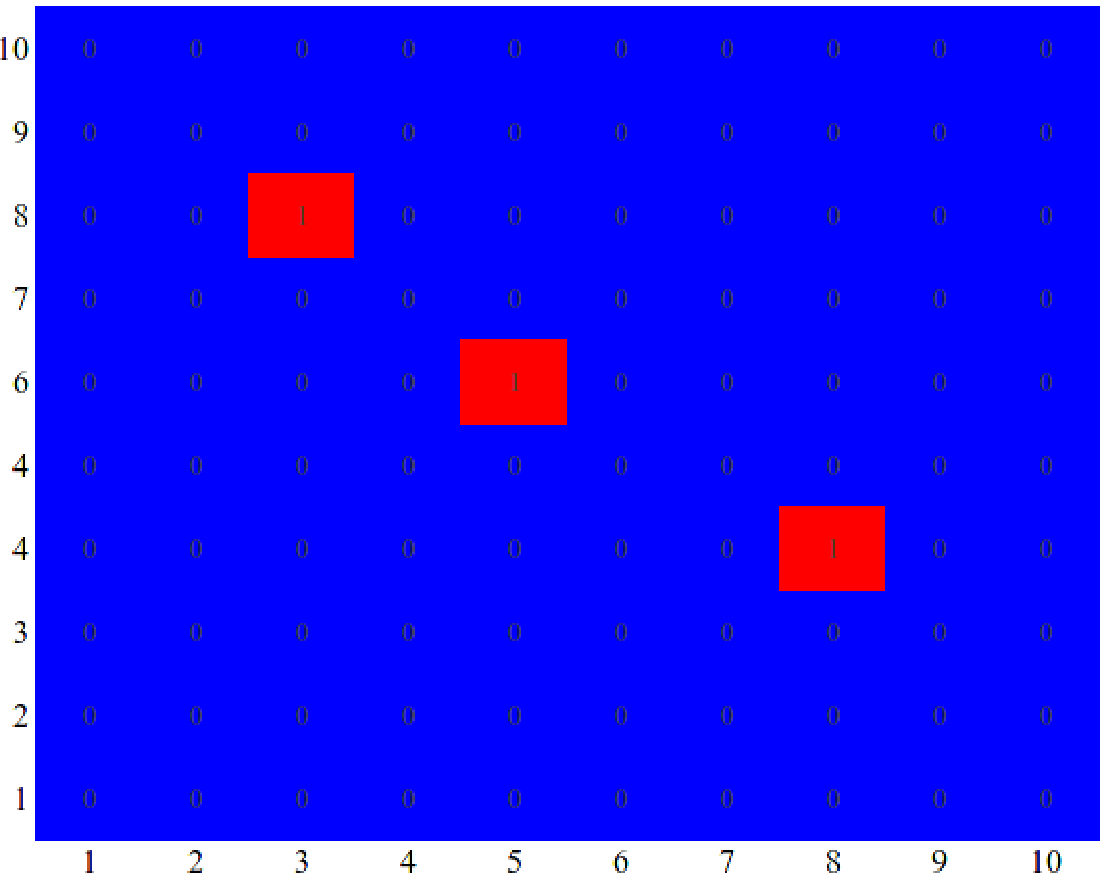
\includegraphics[width=.9\linewidth]{fig_calor1}
    \end{center}
    \vspace{3mm}
    \legenda{(a) Initial zero-temperature distribution over the $10 \times 10$ grid for a finite surface. }
    \end{minipage}
    \hfill
    \begin{minipage}[t]{.46\textwidth}
    \begin{center}
    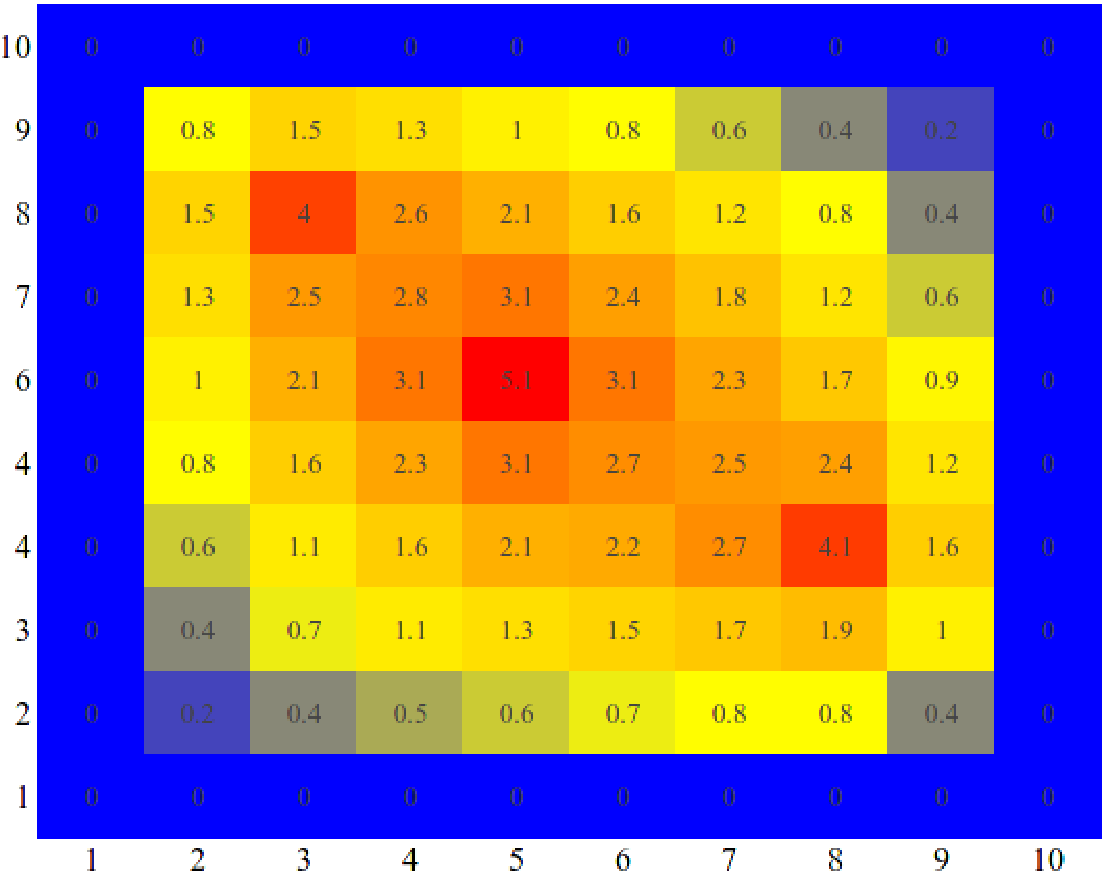
\includegraphics[width=.91\linewidth]{fig_calor2}
    \end{center}
    \vspace{3mm}
    \legenda{(b) Final temperature distribution for the same grid after 500 iterations.}
    \end{minipage}
    \vspace{5mm}
    \legenda{}
    \FONTE{Author's production.}
    \label{fig_calor1e2}
    \end{figure}

The specific algorithm is based on a main loop for time steps. In each iteration (time step), the 2D grid is updated and the temperature of the 3 grid points of the heat sources is increased by 1 unit, modeling the insertion of energy that is performed every time step. The updating of the 2D grid requires the calculation of a five-point stencil over the 2D domain grid \cite {Chen2002} in order to update the temperatures at every time step. A uniform temperature field with zero value is assumed over the surface, and typically, adiabatic or Dirichlet  boundary conditions are assumed, being the latter assumed for this problem. Three constant rate heat sources were placed at localized grid points, and each introduces a unit amount of heat at each time step. The heat transfer simulation is modeled over a finite number of time steps, with all grid points being updated at each time step. The temperature distribution will be determined by the heat sources and the Dirichlet boundary conditions, which implies in zero temperature at the border grid points. 

The five-point stencil allows updating a grid point by averaging the temperatures of the point itself with the temperatures of its four neighboring grid points, left-right and up-down. The temperature field $U$ is defined over a discrete grid $(x,y)$ with spatial resolutions  $\Delta x = \Delta y = h$. Thus, the discretization maps real Cartesian coordinates $(x,y)$ to a discrete grid $(i,j)$, with $U_{x,y}=U_{i,j} \, , \,  U_{x+h,y}=U_{i+1,j} \,$ for the $x$ dimension, and analogously for the $y$ dimension. Therefore, the discretized 2D Poisson equation with a five-point stencil is expressed by \autoref {eq_poisson}.

\begin{equation}
  \frac{\partial^2 U}{\partial x^2} +
  \frac{\partial^2 U}{\partial y^2} \approx
  \frac{U_{i+1,j}+U_{i,j+1}-4U_{i,j}+U_{i-1,j}+U_{i,j-1}}{h^2}
  \label{eq_poisson}
\end{equation}

In the case of parallelization, the domain corresponding to the finite surface is divided into subdomains that are assigned to processes or threads. However, the update of points in the border of subdomains requires the temperatures values of points in the neighboring subdomains, and such data dependency between subdomains implies in communication between processes or synchronization between threads \cite {Langtangen2008a}. Considering the chosen test case, an early implementation of the algorithm was proposed by \citeonline {Balaji2017} using the C language, but later it was ported to F90. \autoref {fig_calor1e2}(b) shows the final temperature distribution over a finite surface after 500 iterations, exemplified by the grid 10 × 10 and three arbitrarily chosen heat sources, shown as \fcred{red} cells. The simulation covers only the internal grid 8 × 8, and the initial zero-temperature distribution is indicated in blue.

The 2D discrete domain is shown in \autoref {fig_malh}(a), with every small circle denotes a grid point and the \fcred{red} cross, the five-point stencil. \fcgreen{Green} lines show the division of the domain into 9 equal subdomains, for the sake of example. The same domain is shown in \autoref {fig_malh}(b), but with each subdomain enlarged by two rows and two columns of extra grid points, shown in yellow, which are copies of the grid points of the four neighboring subdomain. In the borders of the domain, grid points corresponding to the boundary conditions are copied. These extra rows and columns of grid points compose the ghost zone of each subdomain for the specific five-point stencil, with other stencils eventually requiring a different number of rows and columns of grid points. The \fcred{red} arrow denotes the communication/synchronization required to update a grid point of the central subdomain from a ``white point'' of the subdomain above it, with the temperature of this point copied to the corresponding ``yellow point'' of the ghost zone of the considered central subdomain.

    \begin{figure}[hbtp]
    \caption{Discretized 2D domain of the heat transfer case (red cross denotes the five-point stencil).}
    %\vspace{2mm}
    \begin{minipage}[t]{.46\textwidth}
    \begin{center}
    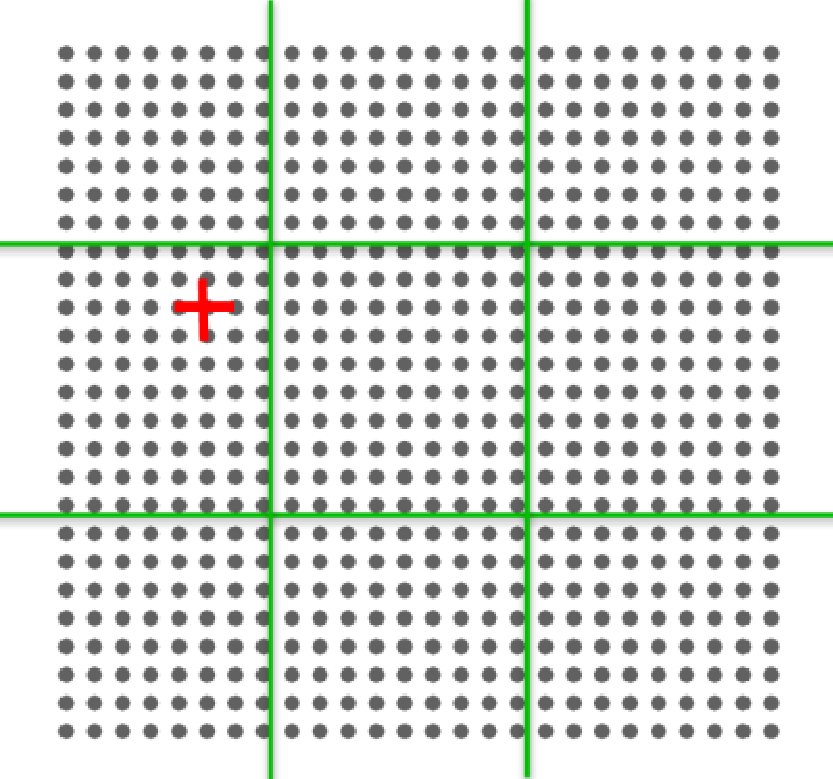
\includegraphics[width=.65\linewidth]{fig_malhdivi}
    \end{center}
    \vspace{3mm}
    \legenda{(a) Discretized 2D domain of the heat transfer problem chosen as test case showing 9 sub domains with their grid points.}
    \end{minipage}
    \hfill
    \begin{minipage}[t]{.46\textwidth}
    \begin{center}
    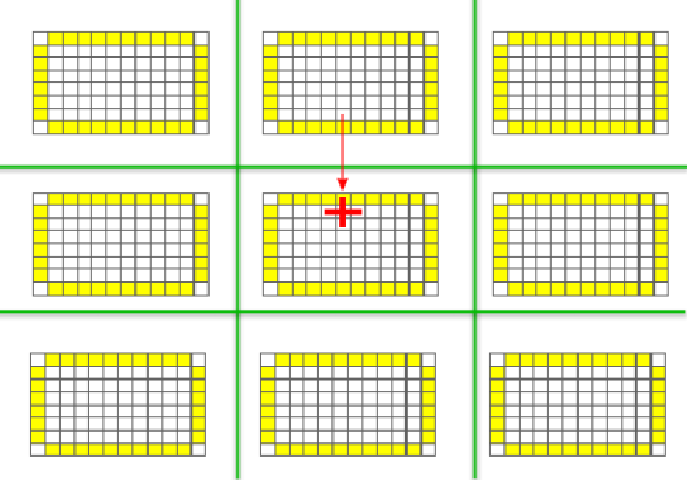
\includegraphics[width=\linewidth]{fig_malhtran}
    \end{center}
    \vspace{3mm}
    \legenda{(b) Discretized 2D domain of the heat transfer problem divided into 9 sub domains enlarged with their ghost zones.}
    \end{minipage}
    \vspace{6mm}
    \legenda{}
    \FONTE{Adapted from \citeonline {Balaji2017}.}
    \label{fig_malh}
    \end{figure}

For simplification, it is assumed a square grid of $n \times n = N$ points, and also a square grid of processors or threads of $p \times p = P$ units, in a way that $n$ is a multiple of $p$. It is then possible to divide the domain into $P$ subdomains, each one containing $[ N/P = (n \times n) / (p \times p) = n/p \times n/p ]$ points. The ghost zone then adds two rows and two columns of grid points, considering the five-point stencil.  Therefore, each subdomain contains $ [ (n+2)/p \times (n+2)/p ] $ points.

Serial and parallel of the Stencil test case F90 implementations were based on a former work \cite {Renato2018}. Other implementations are standard Python, Fortran-to-Python (F2PY), Cython, and Numba (including Numba-GPU). The compute-intensive part of the implementations was hand coded and does not use an existing off-the-shelf external library. In this work, most parallel versions of these implementations are based on MPI: the version is wrapped by the MPI for Python (mpi4py) API into a Python function, allowing the execution of MPI processes in one or more computing nodes from the Python environment. However, the F2PY API is the only exception, since it reuses a binary code generated by an F90 compiler by encapsulating it into a Python function. Parallelization using threads was restricted to the execution of a Numba JIT-compiled function in GPU, which is also discussed ahead.

Stencil test case implementations are described in the next sections.

%
%
%
%----------------------------------------
\subsection{F90 serial and parallel} % Stencil
\label{sec_stenimplf90}
%----------------------------------------

The F90 serial and parallel versions were compiled with the GNU-compiler gfortran, which fully complies to the Fortran 95 standard. The serial F90 version is the implementation of the algorithm described in the previous section. Its corresponding parallel version employs standard MPI asynchronous non-blocking communication functions \textit {MPI\_ISend()} and \textit {MPI\_IRecv()}, which allows overlapping computation and communication, enhancing the parallel performance. However, at the end of each time step, synchronization is required for the updating of each subdomain ghost zones from the neighboring subdomains. As already mentioned, for a square grid with $N = n \times n $ points and $p \times p$ MPI processes, each process is assigned a subdomain with a total of $[(N/p)+2] \times [(N/p)+2]$ points, including the ghost zone. The compute-intensive  part of the code is the updating of the domain grid using the five-point stencil, as shown in the F90 code of the \autoref {lst_stf90}, showing two nested loops that traverse the 2D grid, with the \textit {anew} array stores the values of updated grid elements calculated from their previous values \textit {aold} array.

\begin{lstlisting}[float=hbt, language=Fortran, label={lst_stf90}, caption={Compute-intensive part of the Stencil test case F90 code.}]
do j = 2, by+1
    do i = 2, bx+1
        anew(i,j) = ( aold(i, j) / 2.0 +
                    ( aold(i-1,j) + aold(i+1,j) +
                      aold(i,j-1) + aold(i,j+1) ) / 8.0 )
    enddo
enddo
\end{lstlisting}

%
%
%
%----------------------------------------
\subsection{F2PY serial and parallel} % Stencil
\label{sec_stenimplf2py}
%----------------------------------------

F2PY creates a Python library from the F90/C code, and this library is then imported by the Python code. In this test case, the function arguments of the created library are the number of grid points, the location and heat rate of the sources, the number of iterations, etc. If the F90 code is not already parallelized with MPI, a typical alternative is to use the mpi4py Python library in the Python code. F2PY seems to be convenient when an optimized F90/C code already exists and can be reused. In this test case, the Python code uses F90/C code wrapped into a library built by F2PY, as shown in the \autoref {lst_stf2p}. The Pyhton library libstencil is built by F2PY from F90 code, and includes the function funcstencil. The parameters \textit {gridsize}, \textit {energy}, \textit {niters}, are the same as in the F90 implementation, and the total energy entered into the grid and the elapsed time are returned by the function and stored in the variables \textit {heat} and \textit {etime}.

\begin{lstlisting}[float=hbt, language=Python, label={lst_stf2p}, caption={Compute-intensive part of the F2PY implementation, in the main Python code.}]
heat, etime = libstencil.funcstencil(gridsize, energy, niters)
\end{lstlisting}

%
%
%
%----------------------------------------
\subsection{Standard Python serial and parallel} % Stencil
\label{sec_stenimplpy}
%----------------------------------------

The portability of the F90 code to Python is straightforward, requiring only NumPy as external library, which is the Python numerical-tool library. Most of the loops in the Python code can be executed using NumPy. The structure and sequence of the original code is preserved and executed interactively by the Python interpreter, while the cycle of analyzing results, changing code or parameters, and re-executing, benefits from the JupyterLab environment. However, as any interpreted language, Python is slow. Once the proof-of-concept of the Python code is complete, the code needs to be optimized, focusing on its compute-intensive parts, which are the performance bottlenecks. In this step, the programmer can take advantage of the modular nature of Python to selectively optimize the code, for example by porting a specific module to F90 or by replacing it by an optimized library function. In addition, parallelization can be performed employing the native Python multiprocessing environment. In this work, Python multiprocessing was provided by the MPI for Python (mpi4py) library. The compute-intensive part of the code is the updating of the domain grid using the five-point stencil at each timestep, as shown in the Python code in the \autoref {lst_sfpyt}. Two nested loops traverse the 2D grid, and the \textit {anew} array stores the result of an equation that uses the elements of the \textit {aold} array. Loops are performed internally by NumPy using the colon notation (``:'') in the array indices.

\begin{lstlisting}[float=hbt, language=Python, label={lst_sfpyt}, caption={Compute-intensive part of the Python implementation.}]
anew[1:-1,1:-1] = ( aold[1:-1,1:-1] / 2.0 +
                  ( aold[2:,1:-1] + aold[:-2,1:-1] +
                    aold[1:-1,2:]  + aold[1:-1,:-2] ) / 8.0 )
\end{lstlisting}

%
%
%
%----------------------------------------
\subsection{Cython serial and parallel} % Stencil
\label{sec_stenimplcy}
%----------------------------------------

Cython is a compiler for both the Cython and Python languages, which is typically used to create Python libraries. These libraries are later called from standard Python code. In this test case the original Python code was reused, with few changes, in order to be compiled by Cython. The Cython parallel version employs mpi4py. The part that updates the 2D grid using the five-point stencil is shown in the \autoref {lst_stcyt}.

\begin{lstlisting}[float=hbt, language=Python, label=lst_stcyt, caption={Compute-intensive part of the Cython implementation.}]
cpdef stp(double[:,::1] anew, double[:,::1] aold, Py_ssize_t by, Py_ssize_t bx):
    for i in range(1, bx+1):
        for j in range(1, by+1):
            anew[i,j] = ( aold[i,j] / 2.0 +
                        ( aold[i-1,j] + aold[i+1,j] +
                          aold[i,j-1] + aold[i,j+1] ) / 8.0 )
\end{lstlisting}

In this Cython implementation, the code included comments starting with ``\#cython:'' that are actually compiler directives for disabling limit checking, disabling negative indexing, inferring the types of variables, among others.

%
%
%
%----------------------------------------
\subsection{Numba serial and parallel} % Stencil
\label{sec_stenimplnumb}
%----------------------------------------

In this implementation, the compute-intensive part of the Python code was embedded into a function decorated for Numba JIT-compilation. The remaining Python code is interpreted by standard Python. Parallelization for the Numba-compiled function is provided by mpi4py for multicore processors. In the case of the standard multicore processor parallelization of the Numba code, the compute-intensive function that updates the domain grid using the five-point stencil is shown in the \autoref {lst_stnum}. Loops are performed internally by NumPy using the colon notation (``:'') in the array indices. \textit {@jit} is the Python decorator for Numba JIT compilation.

\begin{lstlisting}[float=hbt, language=Python, label=lst_stnum, caption={Compute-intensive part of the Numba implementation.}]
@jit(nopython=True)
def kernel(anew, aold):
    anew[1:-1,1:-1] = ( aold[1:-1,1:-1] / 2.0 +
                      ( aold[2:,1:-1] + aold[:-2,1:-1] +
                        aold[1:-1,2:] + aold[1:-1,:-2] ) / 8.0 )
\end{lstlisting}

%
%
%
%----------------------------------------
\subsection{Numba-GPU} % Stencil
\label{sec_stenimplngpu}
%----------------------------------------

In this section, Numba was also employed for execution using a GPU, since Numba supports part of the Nvidia CUDA API, requiring the definition of the kernel function that will be executed on the GPU. The Numba-GPU implementation required more modifications to the standard Python serial code, than the other implementations. The compute-intensive part of the code was encapsulated into a JIT-compiled function for GPU execution by means of a Numba decorator. As usual, the remaining code of the test case algorithm is executed by the standard Python interpreter, since it is not compute-intensive.

The compute-intensive part of the code is the updating of the 2D grid/array using the five-point stencil, as shown in the code of \autoref {lst_stgpu}. The kernel function executed in the GPU assigns the iterations of two nested loops that traverse the 2D grid by blocks of threads in a way that each thread calculates the stencil at a grid point. Each block is divided into 32-thread warps and assigned to a particular GPU streaming multiprocessor. Two copies of the 2D array are created in the GPU memory, being swapped one for another: the \textit {anew} array stores the 2D grid that is updated from the 2D grid stored in the \textit {aold} array, and vice-versa along the time steps. Numba-GPU requires more code changes than the CPU version, such as defining GPU blocks and grids, and transferring data from host memory to device/GPU memory, and vice-versa. \textit {@cuda.jit} is the Python decorator for Numba-GPU JIT compilation.

\begin{lstlisting}[float=hbt, language=Fortran, label={lst_stgpu}, caption={Compute-intensive part of the Numba-GPU implementation.}]
@cuda.jit
def kernel(anew, aold):
    n = anew.shape[0] - 1
    i, j = cuda.grid(2)
    if (i > 0 and j > 0) and (i < n and j < n):
        anew[i,j] = ( aold[i,j] / 2.0 + 
                    ( aold[i-1,j] + aold[i+1,j] +
                      aold[i,j-1] + aold[i,j+1]) / 8.0 )
\end{lstlisting}

The algorithm comprises the main loop with iterations that correspond to the time steps of the simulation. At each time step/iteration, the 2D array must be updated. In the serial version, such updating is entirely executed by the kernel function in the GPU. The 2D array is transferred to the GPU in the first time step, the GPU updates the 2D array and inserts energy in each time step, and only at the last time step the final 2D array is transferred back to the host memory.

However, in the parallel version, the 2D array cannot be fully updated by each MPI process (in the GPU), since the updating of the borders of its subdomain requires the updated values of the ghost zone, which are calculated by the processes that update the neighbouring subdomains. Therefore, each process needs to transfer its updated borders from the GPU to the host memory in order to send these values to the neighbouring processes. Besides, each process receives the updated borders from the neighbouring processes in order to transfer these values to the GPU, which compose the updated ghost zone of the subdomain. After the last time step is completed, the GPU of each process must transfer the final array back to its host memory. Therefore, MPI communication and Host-GPU transfer in both directions, both related to the updating of ghost zones, make the performance of parallel versions very low compared to serial versions. 

%
%
%
%
%
%
%
%  _____ _____ _____ 
% |  ___|  ___|_   _|
% | |_  | |_    | |  
% |  _| |  _|   | |  
% |_|   |_|     |_| 
%----------------------------------------
\section{FFT test case and implementations}
\label{sec_fft}
%----------------------------------------

This section describes a specific FFT algorithm, the Fast Fourier Transform in the West (FFTW), applied to a synthetic 3D multidimensional array. An array of synthetic data has elements assigned by the programmer, as an alternative to real-world data. 

FFT is an algorithm that computes the discrete Fourier transform (DFT), which is a numerical algorithm for converting a finite sequence of $N$ equally spaced samples in the temporal or spatial domain, into the corresponding sequence in the frequency domain. For instance, the FFT allows decomposing a signal varying in time consisting of multiple pure frequencies. The Fast Fourier Transform (FFT) is an approach that reduces the DFT computation complexity from $\mathcal{O}(N^2)$ to $\mathcal{O}(N\log{}N)$. 
 
The 1D DFT of a sequence of $N$ complex numbers results in a sequence of $N-1$ complex numbers given by \autoref {eq_fft}.

\begin{equation}\label{eq_fft}
X_k = \sum_{n=0}^{N-1} x_n \cdot
	  e^{\textstyle - {\frac{\textstyle 2 \pi i k n}{N} } }
	  \quad , \qquad ( k = 0, ..., N-1 )
\end{equation}

The calculation of multidimensional 3D FFTs is given by the product of the corresponding 1D FFTs along each dimension, as shown in the \autoref {eq_fftresu}. Each 3-element tuple of complex numbers in the time or space domain is mapped to a corresponding 3-element tuple of complex numbers in the frequency domain for the same 3D grid. The same equation can be adapted for higher dimensions.

\begin{equation}\label{eq_fftresu}
X ( k_1, k_2, k_3 ) = 
    \sum_{ n_3 = 0 } ^ { N_3 - 1 }
    \sum_{ n_2 = 0 } ^ { N_2 - 1 } 
    \sum_{ n_1 = 0 } ^ { N_1 - 1 }
    \; x ( n_1, n_2, n_3 ) \;
    e^{
        \frac{ - 2 \pi i k_3 n_3 } { N_3 } \times
        \frac{ - 2 \pi i k_2 n_2 } { N_2 } \times
        \frac{ - 2 \pi i k_1 n_1 } { N_1 }
    }
\end{equation}

The parallelization is performed by dividing and distributing the 3D array of $N^3$ complex numbers into $N/p$ slabs that are assigned to $p$ MPI processes. Two successive 1D FFTs are performed on the y and z dimensions for each slab, and then a new set of $N/p$ slabs is obtained by the transposition of the former ones, in a way that the new slabs are assigned to the $p$ MPI processes. This requires an all-to-all communication. Finally, each MPI process performs a 1D FFT on the x dimension of its slab. This scheme is shown in \autoref {fig_fft}, but considering a more generic multidimensional array of dimension $L\times M \times N$ and $4$ processes,  

    \FIGURE [] [0mm] {Parallelization of the 3D FFT, showing the decomposition of a $L\times M \times N$ domain into 4 slabs assigned to 4 MPI processes.} {Adapted from \citeonline {Schulz2008}.} {fig_fft}

The standard implementations of Python, Cython and Numba FFT employ the mpi4py-fft library (\autoref {sec_apprmfft}) which depends on the FFTW library, and also the mpi4py library for parallelization, and which automatically distributes large sequences or data arrays. In the case of the F90 and F2PY implementations, the FFTW library available on the SDumont was used (module \textit {mathlibs/fftw/3.3.8\_openmpi-3.1\_gnu}) with the MPI library. Therefore, differently from the Stencil test case, the compute-intensive part of the code uses off-the-shelf external libraries.

In order to obtain performance, F90 is straightforward, followed by F2PY, which required relatively few changes to the original F90 code, and Python. FFT test case implementations are described in the next sections.

%
%
%
%----------------------------------------
\subsection{F90 serial and parallel} % FFT
\label{sec_fftimplf90}
%----------------------------------------

The F90 serial and parallel versions were compiled with the GNU-compiler gfortran, which complies to the Fortran 95 standard. These F90 implementations employ the FFTW library available on the SDumont, and the MPI library. Parallelization is performed as described above, in the \autoref {sec_fft}. The FFTW library includes a planning step before running the FFT, in order to optimize the processing performance. The compute-intensive part of the code is shown in the \autoref {lst_ftf90}, being performed by the FFTW library (\textit {fftw\_mpi\_execute\_dft}). In the code, \textit {plan} is given as an option, \textit {data1} is the input 3D array, while \textit {data2} is the output one.

\begin{lstlisting}[float=hbt, language=Fortran, label={lst_ftf90}, caption={compute-intensive part of the FFT test case F90 code.}]
call fftw_mpi_execute_dft(plan, data1, data2)
\end{lstlisting}

%
%
%
%----------------------------------------
\subsection{F2PY serial and parallel} % FFT
\label{sec_fftimplf2py}
%----------------------------------------

The F2PY implementation reuses the F90 source code, including the MPI and FFT libraries, with minor changes. The original compute-intensive source code is transformed into Python functions with the corresponding arguments. The F90 source code is then built using F2PY and the -O3 compilation flag, and wrapped by F2PY into a standard Python library, which contains most of the original code, including: 
(i) initializing the 3D array with values derived from the array indices, 
(ii) calculating the FFTW transform, and 
(iii) calculating the array checksum in order to check the correctness of the result. 
The remaining Python code is short, since it just imports the library to call the functions built by F2PY, and then displays the result. 

Instead of passing input parameters as function arguments, another possible approach can be created by hardcoding the arguments, i.e., to declare their values as parameters inside the program. Such approach was used in this test case for convenience, since it is easy to edit the code, recompile and re-execute it using the JupyterLab notebook. Changes in the Python code are minimal, and the use of Slurm is also similar. Two different versions of the library were developed, serial and parallel, for ease of use, but is would be possible to employ a single version, and choose serial or parallel execution using the Slurm script. 

The compute-intensive part of the F2PY implementation is due to the Python function calls to perform the FFTW, shown in the \autoref {lst_ftf2p} (Pyhton library libfft and function funcfft built by F2PY using the size \textit {gridsize3d} of the array as argument). This function call returns the checksum of the array elements and the elapsed time, in the \textit {csum} and \textit {etime} variables. 

\begin{lstlisting}[float=hbt, language=Python, label={lst_ftf2p}, caption={Compute-intensive part of the FFT test case Python code.}]
csum, etime = libfft.funcfft(gridsize3d)
\end{lstlisting}

%
%
%
%----------------------------------------
\subsection{Standard Python serial and parallel} % FFT
\label{sec_fftimplpy}
%----------------------------------------

In the Python serial implementation, the Python library pyFFTW is used, which is an encapsulated version of the C-compiled FFTW, being the compute-intensive part of the implementation. The remaining part is the standard Python code, executed in an interpreted way. However, the initialization of the 3D multidimensional array was written in Python and requires nested loops, which are very slow when executed in interpreted form. Therefore, the Python code that performs the initialization was optimized by calls to functions of the NumPy library. 
The parallel Python implementation simply calls the mpi4py-fft library, that adds an MPI parallelization layer to the same FFTW library.

In this implementation, the computation-intensive part of the code is shown in the \autoref {lst_ftpyt}, being performed by the pyFFTW library (\textit {pf.interfaces.numpy\_fft.fftn}). The array \textit {u} contains the input 3D multidimensional array, \textit {uf} contains the result, \textit {overwrite\_input=True} indicates that the input array can be overwritten, while \textit {auto\_contiguous=False}, and \textit {auto\_align\_input=False} both indicate that the multidimensional array can be copied into contiguous memory positions that are also aligned in memory, in order to optimize memory access. 

\begin{lstlisting}[float=hbt, language=Python, label={lst_ftpyt}, caption={Compute-intensive part of the FFT test case Python code.}]
uf = pf.interfaces.numpy_fft.fftn(u,
                                  overwrite_input=True,
                                  auto_contiguous=False,
                                  auto_align_input=False)
\end{lstlisting}

%
%
%
%----------------------------------------
\subsection{Cython serial and parallel} % FFT
\label{sec_fftimplcy}
%----------------------------------------

Cython is a static optimizing compiler that translates Python or Cython source code into C language target code that is then compiled to generate an optimized machine code. Cython implementations use the same Python libraries pyFFTW (serial), and mpi4py-fft (parallel) as the standard Python corresponding implementations. Therefore, the remaining Python code is the same for both corresponding serial and parallel implementations. Function input arguments were hardcoded, taking advantage of the JupyterLab notebook.

The compute-intensive part of the code is the function call to the library pyFFTW (serial version), or to mpi4py-fft library (parallel version), as shown in the \autoref {lst_ftcyt} for both versions. The \textit {data} argument contains the input 3D multidimensional array, while \textit {result} is the output transformed array. In the parallel version, MPI.COMM\_WORLD is the default MPI communicator, $[N,N,N]$ is the dimensions of the 3D array, dtype is the type of each element in the array (complex number), and the backend specifies the pyFFTW library, which is the same used in the serial version.

\begin{lstlisting}[float=hbt, language=Python, label={lst_ftcyt}, caption={Compute-intensive part of the FFT test case Cython code.}]
# serial version:
result = pyfftw.interfaces.numpy_fft.fftn(data)
# parallel version:
plan = PFFT(MPI.COMM_WORLD, [N, N, N], dtype=np.complex128, backend='pyfftw')
result = plan.forward(data)
\end{lstlisting}

%
%
%
%----------------------------------------
\subsection{Numba serial and parallel} % FFT
\label{sec_fftimplnumb}
%----------------------------------------

The Numba implementation employed JIT compilation, and similarly to the standard Python and Cython implementations, the serial version uses the pyFFTW library and the parallel version uses the mpi4py-fft library. Differently from the Numba implementation of the Stencil test case, JIT compilation was not used in the computationally intensive part of the FFTW, since it is executed by the pyFFTW library which has already been AOT compiled and optimized. However, Numba was used in the rest of the code including the function that initializes the 3D multidimensional array, being faster than the corresponding part of the standard Python implementation.

The compute-intensive part of this implementation is also the function call of the library pyFFTW for the serial version, or mpi4py-fft for the parallel version, and is shown in the \autoref {lst_ftnum}, both already AOT compiled, for the serial and parallel versions. The parameter \textit {data} is the array containing the input 3D multidimensional array. In the parallel version, MPI.COMM\_WORLD is the standard MPI communicator, $[N,N,N]$ are the dimensions of the 3D array, dtype is the type of each element of the array (complex number), and backend specifies the pyFFTW library, which is the same used in the serial version.

\begin{lstlisting}[float=hbt, language=Python, label={lst_ftnum}, caption={Compute-intensive part of the FFT test case Numba code.}]
# serial version:
result = pyfftw.interfaces.numpy_fft.fftn(data)
# parallel version:
plan = PFFT(MPI.COMM_WORLD, [N, N, N], dtype=np.complex128, backend='pyfftw')
result = plan.forward(data)
\end{lstlisting}

%
%
%
%----------------------------------------
\subsection{CuPy} % FFT
\label{sec_fftimplngpu}
%----------------------------------------

The CuPy implementation was executed on a B715 node or on a Seq-X (\autoref {sec_sdenviron}), both employing a single GPU. The CuPy library is GPU-specific, NumPy-compatible, and encapsulates the CUDA toolkit. The compute-intensive part is the FFTW, performed by a CuPy library function and executed in the GPU. Other CuPy functions were employed to transfer the input array to/from the GPU memory, and to calculate the checksum of the array elements. The NumPy \textit {fromfunction} function was used to initialize the 3D multidimensional array to avoid using the Python interpreter slow loops. The same CuPy code was executed on a B715 node using Slurm or on a Seq-X directly from the operating system command line, using a Tesla K40t GPU or a Volta V100 GPU, respectively. The compute-intensive part of the Python code of the CuPy implementation is the function call of the library routine shown in the \autoref {lts_ftgpu}. The \textit {data} argument is the input 3D array, and \textit {result} is the transformed output array. Provided that there is the availability of an optimized CuPy function for the compute-intensive part of the code, this is a very simple way for employing a GPU.

\begin{lstlisting}[float=hbt, language=Python, label={lts_ftgpu}, caption={Compute-intensive part of the FFT test case CuPy code.}]
result = cupy.fft.fftn(data)
\end{lstlisting}

%
%
%
%
%
%
%
%  _____                   _   
% |  ___|__  _ __ ___  ___| |_ 
% | |_ / _ \| '__/ _ \/ __| __|
% |  _| (_) | | |  __/\__ \ |_ 
% |_|  \___/|_|  \___||___/\__|
%----------------------------------------
\section{Random Forest test case and implementations}
\label{sec_forest}
%----------------------------------------

This test case describes the implementation of the machine learning algorithm Random Forest (RF), applied for the classification of asteroid orbits. An RF is a set of decision trees generated by an ensemble method. As in the other test cases, the corresponding RF implementations were made in F90 and Python, in both sequential and parallel versions. 

%
%
%
%----------------------------------------
\subsection{Random Forest and ensemble methods} % RF
%----------------------------------------

A decision tree is a machine learning algorithm (MLA), more specifically, a non-parametric (does not require hyperparameters) supervised (applied to known classes) learning method used for classification and regression. A decision tree is similar to a graph, composed of nodes and branches, with each node associated to an attribute of the input data, and each branch associated to the class or value of the node attribute. Nodes are ordered according to its importance for discriminating the instances. At the end of the tree, branches are assigned with the corresponding major class. A decision tree is called a regression tree if it uses numerical data, or a classification tree if it uses categorical (class) data. Similarly to other machine learning algorithms, input data is divided into information variables (input) and a decision variable (output). In the training phase, a decision tree is generated from known instances of the training dataset. Then, in the test phase, the decision tree is used to perform classification or regression on new input data in order to estimate the decision variable for each new instance of the test dataset. 

An ensemble method may improve the performance of any MLA by combining a finite set of instances of the original MLA, being these instances called members of the ensemble. This ensemble-generated set of members actually represents a new MLA that is expected to yield a better result than the original MLA. In general, ensemble methods may have  members being training independently one from one another \textit {in parallel}, or being trained consecutively in sequence. Considering a given MLA, the use of an ensemble method reduces the bias error, which is due to the algorithm itself or its hyperparameters, by means of reducing the error due to the variance, which is due to sensitivity to small fluctuations in the input data. As a consequence, ensemble methods helps to avoid overfitting. The most standard ensemble methods are Bagging and Boosting, with each one having many variations.

Bagging \cite {Breiman2001}, from Bootstrap Aggregating, applies some sampling scheme to the input data in order to generate different training datasets for the ensemble members, but is possible to use an ensemble of different MLAs or of the same MLA with different hyperparameters. Each dataset contains a different set of instances, but each instance has the  complete set of input attributes. Another scheme would be to use a slightly different set of attributes in the training of each member, but the complete set of instances of the input data, or yet a combination of both approaches. In addition, the use of different training data can be applied for ensembles composed of different MLAs. After the training, in the test phase, the result of the ensemble-MLA for each new instance is given by averaging the results of the members (for numerical output, in classification or regression), or by a polling scheme (for categorical output, in classification). Bagging is inherently parallelizable, since members are trained independently, by assigning one or a block of members to each MPI process or POSIX thread. An RF is an ensemble of decision trees that employs Bagging.

Boosting \cite {Breiman2001} is an ensemble method in which training is performed consecutively on the members, but weighting the error of each instance. In the training of the first member, weights are initially equal to unity, but in the successive trainings of the members, the importance of each instance is weighted by its corresponding classification/regression error. Boosting it is not memberwise parallelizable, since each member is trained consecutively, but it is usually faster than Bagging, as it demands a much lower number of members. Eventually, the execution of each member may be parallelizable. After the training, in the test phase, the result of the ensemble-MLA for each new instance is given by the last member of the ensemble.

In this test case, the ensemble method is an RF, and thus bagging was applied to generate $N$ training sets for each of the $N$ trees. Each set is obtained by randomly sampling, with replacement, the original dataset. \autoref {fig_rfdiag} presents the flowchart of an RF composed of the set of decision trees in the test phase, i.e., after the decision trees were trained. Each instance from the test dataset is then classified by each of the decision trees, yielding a result, which can be numerical or categorical. The final result of the RF is then computed by averaging the numerical results or by a polling scheme for categorical results. 

    \FIGURE {RF flowchart.} {Author's production.} {fig_rfdiag}

%
%
%
%----------------------------------------
\subsection {The asteroid orbit classification problem} % RF
%----------------------------------------

This problem is about training an MLA, a Random Forest, to perform asteroid orbit classification. A dataset of 100,000 asteroids was randomly selected and divided into training and test sets, with respectively 66,000 and 34,000 instances, each defined in a separate ARFF file. Each instance of the dataset corresponds to an observed asteroid and contains 37 attributes that the RF employs to classify the asteroid class, among the 13 possible classes for asteroid orbit, as described in \autoref {tab_rfclass} and in \autoref {tab_rfattri}.  

    \TABLE {The 13 asteroid orbit classes for the \textit {class} decision attribute in the asteroid orbit dataset.} {Adapted from the NASA Planetary Data System (2022).} {tab_rfclass}

    \TABLE {The 37 selected information attributes plus 1 for the asteroid orbit dataset (the 38th one is the decision attribute, the class, as described in the preceding table).} {Adapted from the NASA Planetary Data System (2021).} {tab_rfattri}

Asteroid orbit data were obtained from the Solar System Dynamics (SSD) of the Jet Propulsion Laboratory (JPL) \footnote{\url{http://ssd.jpl.nasa.gov/}}. It provides astronomical data about the orbits, physical characteristics, and discovery circumstances for most of the known natural bodies in the Solar System. A subset of it, the Small Bodies Database (SBDB), provides information about small bodies like known asteroids and comets. For convenience, raw data were pre-processed using Weka software (Waikato Environment for Knowledge Analysis, developed at the University of Waikato, New Zealand) \footnote{\url{http://www.cs.waikato.ac.nz/ml/weka/}}, and the resulting datasets are in ARFF format.

%
%
%
%----------------------------------------
\subsection{Random Forest implementations} % RF
%----------------------------------------

In the Random Forest test case, all implementations were executed using processor cores of one or more computing nodes (no GPU). Python was used with the Scikit-learn library (\autoref {sec_apprsklr}), and since this library is a highly optimized and constantly updated, performance results were better than those obtained by the F90 or F2PY implementations, which are based on the obsolete PARF library (\autoref {sec_apprparf}). As a consequence, differently from the previous test cases, the F90 implementation was not taken as a reference. 

It is important to note that, with the exception of the F90 and F2PY implementations, the other Python implementations of this test case (standard Python, Cython and Numba) do not employ the MPI communication library for parallelization, using instead the IPP library. Parallelization is accomplished by running multiple training and prediction processes on decision trees, using multiple MPI or IPP processes (depending on implementation). In the case of Python, the Scikit-learn library uses the IPP library as a backend, which works using engines and other components that run in processes, as discussed in the \autoref {sec_appripyt}.

Random forest test case implementations are described in the next sections.

%
%
%
%----------------------------------------
\subsubsection{F90 serial and parallel} % RF
\label{sec_rfimplf90}
%----------------------------------------

The serial and MPI-based parallel F90 implementations use the PARF (\autoref {sec_apprparf}), an F90 library written for Random Forest classification. The compute-intensive part of the code, executed by the PARF library is the \textit {build\_tree} routine that builds the trees, and corresponds to 46\% of the total processing time according to the \texttt {gprof} operating system profiler. 

%
%
%
%----------------------------------------
\subsubsection{F2PY serial and parallel} % RF
\label{sec_rfimplf2py}
%----------------------------------------

In the F2PY implementation, the original PARF F90 code with a command line interface was re-written as a subroutine and then built by F2PY into a Python library. The Intel compiler with the optimization flag -O3 was used instead of the GNU compiler, since PARF requires some Intel resources. The input are the files containing the datasets, and the outputs are the classification error, another metric for classification accuracy (kappa), and the elapsed time measured using the F90 library wall time function. In the parallel version, all MPI declarations and calls are in the PARF code, and the F2PY is built using the Intel MPI. 

The remaining Python code is basically the same for both serial and parallel versions, being the only difference the name of the library built by F2PY for the serial and parallel versions. The number of MPI processes is defined in the Slurm script (1, 4, 16, 24, 48, 72, and 96 processes), and execution times are the average of 3 runs.

The compute-intensive part of the code shown in \autoref {lst_rfp2p} refers to the F2PY-built function. In the listing, \textit {result} contains the set of output parameters, \textit {lib\_p2py\_parf} is the name of the library created by P2PY, \textit {random\_forest} is the function with the compiled PARF code, and the files \textit {train.arff} and \textit {test.arff} contain the datasets for the training and testing phases, respectively.

\begin{lstlisting}[float=hbt, language=Python, label={lst_rfp2p}, caption={Compute-intensive part of the Random Forest test case F2PY code.}]
result = lib_p2py_parf.random_forest("train.arff", "test.arff")
\end{lstlisting}

%
%
%
%----------------------------------------
\subsubsection{Standard Python serial and parallel} % RF
\label{sec_rfimplpy}
%----------------------------------------

The standard Python serial and parallel implementations, as well as the Cython and Numba ones, use the Scikit-learn library that employs the IPP library as parallel backend. The Scikit-learn Random Forest library is faster than PARF. The Pandas library was used to store the datasets, which are read from ARFF files using the SciPy library.

This test case requires the training and test phases of a classification algorithm. The use of Scikit-learn requires a configuration step to select an estimator/classifier (in this case, the Random Forest), and also to select the specific parameters of the estimator. In the next step, training is performed using the training dataset, and then testing, using the test dataset.

The compute-intensive part of the code is shown in the \autoref {lst_rfpyt} and is performed by the Scikit-learn library. In the parallel version, the line that declares the backend is added. The \textit {clf} is the Random Forest classifier, the \textit {fit} is the function that performs the classification, and the \textit {X} contains a matrix of dimension $66,000 \times 36$, since there are 66,000 training instances and 36 attributes. And finally, \textit {y} is a vector of dimension 66,000 containing the known classification for these instances into one of 13 possible classes. The result is the trained Random Forest model, also stored as \textit {clf}, which can then be employed in the test phase.

\begin{lstlisting}[float=hbt, language=Python, label={lst_rfpyt}, caption={Compute-intensive part of the Random Forest test case Python code.}]
with parallel_backend('ipyparallel'):
    clf.fit(X, y)
\end{lstlisting}

%
%
%
%----------------------------------------
\subsubsection{Cython serial and parallel} % RF
\label{sec_rfimplcy}
%----------------------------------------

In the Cython implementation, the same code of the Python standard implementation is reused, and thus includes the same calls to the Scikit-learn library. As this library is already optimized for performance, porting the Python code to Cython would not significantly improve performance. The Cython parallel version is also similar to the corresponding standard Python, using IPP as the parallel backend.

Please see the \autoref {lst_rfpyt} in the \autoref {sec_rfimplpy} containing the compute-intensive part of the Cython code, as it is identical to the standard Python implementation.

%
%
%
%----------------------------------------
\subsubsection{Numba serial and parallel} % RF
\label{sec_rfimplnumb}
%----------------------------------------

In the Numba implementation, the same code as the standard Python implementation is reused and therefore includes the same calls to the optimized Scikit-learn library. Since this library is already optimized for performance, there would be useless to port the source code to Numba in order to optimize it. However, there is a small gain of performance by using Numba JIT compilation for the remaining part of the Python code. The IPP parallel backend is also employed for the Numba parallel version. The Numba implementation is then executed in three different ways: 
(i) interpreted by standard Python (only for small parts of the original code), 
(ii) executed using optimized library functions (compute-intensive part), and 
(iii) executed using Numba JIT-compilation (remaining part).

Please see the \autoref {lst_rfpyt} in the \autoref {sec_rfimplpy} containing the compute-intensive part of the Numba code, since it is identical to the standard Python implementation.

%   ____ _                 _              _  _   
%  / ___| |__   __ _ _ __ | |_ ___ _ __  | || |  
% | |   | '_ \ / _` | '_ \| __/ _ \ '__| | || |_ 
% | |___| | | | (_| | |_) | ||  __/ |    |__   _|
%  \____|_| |_|\__,_| .__/ \__\___|_|       |_|  
%                   |_|   
%%%%%%%%%%%%%%%%%%%%%%%%%%%%%%%%%%%%%%%%
\chapter{TEST CASES PARALLEL PERFORMANCE}
\label{ch_analysis}
%%%%%%%%%%%%%%%%%%%%%%%%%%%%%%%%%%%%%%%%

This chapter covers the analysis of the parallel performance of the different serial and parallel implementations (F90 and Python) for each one of the three selected test cases. Most of the parallel implementations are MPI-based, but there are some others that employ specific Python libraries. The only implementations that were executed using thread parallelism were Numba-GPU and CuPy for GPU execution, and the loky implementation for CPU execution using threads. This chapter is divided as follows:

\begin{itemize}

\item\autoref {sec_analintr} Test environment: standard parallel performance definitions, description of the SDumont execution nodes, and a listing of the versions of the employed compilers, Python, etc.;

\item\autoref {sec_analsten} Stencil test case: a five-point stencil finite difference method to solve partial differential equations resulting from Poisson equations, applied to a 2D heat transfer problem on a finite surface;

\item\autoref {sec_analfft} Fast Fourier Transform (FFT) test case: an algorithm that computes the multidimensional Fourier transform of an 3D array of synthetic data; 

\item\autoref {sec_analrf} Random Forest test case: a random forest algorithm applied for the classification of asteroid orbits of a NASA dataset.

\end{itemize}

\textbf{General guidelines for the tests}: all processing times shown here are the average of 3 executions. The calculation of speedups and parallel efficiencies always took the serial execution time of the F90 implementation as a reference, except for the Randon Forest test case, which used the serial execution time of the standard Python implementation as a reference. The serial and parallel test cases were executed by means of the Slurm job scheduler, except where otherwise stated. The JupyterLab interactive environment was employed in all tests.

%
%
%
%----------------------------------------
\section{Test environment}
\label{sec_analintr}
%----------------------------------------

Standard parallel performance metrics are used here, like the speedup $S_p$, given by the ratio between the serial $t_s$ and the parallel execution time $t_p$, using $p$ processes or threads (\autoref {eq_spd}), being the ideal speedup, called linear speedup, equal to $p$.

\vspace{-2mm}
\begin{equation}\label{eq_spd}
S_p = \frac{t_s}{t_p}
\end{equation}

In this work, for each considered implementation of any test case, the speedup is calculated using the time of the serial version and the corresponding time of the parallel version, i.e., same programming language and compiler. However, the best serial time of each test case is considered, in order to allow a more fair comparison of speedups. Another standard metric is the parallel efficiency $E_p$, given by the ratio between the speedup $S_p$ and the corresponding number of $p$ processes or threads (\autoref {eq_ep}). Thus, a linear speedup corresponds to a parallel efficiency of 100\%, or unitary. It is important to note that the parallel efficiency can be higher than 100\%, depending on the value adopted as a reference for the speedup calculation. It can also happen for serial and parallel versions generated with the same programming language and compiler, if the parallelization implies in an optimization of the memory access, and thus lowering execution times of each process/thread.

\vspace{-2mm}
\begin{equation}\label{eq_ep}
E_p = \frac{S_p}{p}
\end{equation}

%
%
%
%----------------------------------------
\subsection{The Santos Dumont computing environment}
\label{sec_sdenviron}
%----------------------------------------

This section describes briefly the SDumont computing environment in terms of software and hardware. Three different computer nodes \footnote{\url{http://sdumont.lncc.br/machine.php?pg=machine}} of the LNCC Santos Dumont supercomputer were employed:

\begin{itemize}

\item \textbf{Thin node B710} (B710), with 2 Intel Xeon E5-2695v2 Ivy Bridge (2.4 GHz) 12-core processors (total of 24 cores per node) and 64 GB main memory; compilers and libraries include GNU Fortran 7.4, GNU Fortran 8.3, OpenMPI 4.0.1, Intel Fortran 19.0.3, Intel MPI, Python 3.6.12, Cython 0.29.20, NumPy 1.18.1, and  Numba 0.41.0;

\item \textbf{Thin node B715} (B715), with 2 Intel Xeon E5-2695v2 Ivy Bridge (2.4 GHz) 12-core processors (total of 24 cores per node), 64 GB main memory, and 2 GPUs Nvidia Tesla K40t; in addition to the compilers and libraries of the B710 nodes, there are CUDA libraries;

\item \textbf{Sequana X node} (Seq-X)

    \begin{itemize}
    
    \item \textbf{Execution node}, with 2 Intel Xeon Gold 6252 (2.1 GHz) 24-core processors (total of 48 cores per node), 4 GPUs Nvidia Volta V100 and 384 GB main memory; in addition to the compilers and libraries of the B710 nodes, there are CUDA libraries;
    
    \item \textbf{sdumont18 login node} \footnote{\url{http://sdumont.lncc.br/support_manual.php?pg=support\#6.8}} , with 2 Intel Xeon Gold 6152 (2.1 GHz) 22-core processors (total of 44 cores per node), 4 GPUs Nvidia Volta V100 and 768 GB main memory.
    
    \end{itemize}

\end{itemize}

The employed compilers and libraries for F90 and Python are available in the SDumont computing environment. Serial and parallel implementations of the F90 used two suites of tools and compilers: GNU version 4.8.5 and Intel versions 19.0.3 or 19.1.2, included in the Intel Parallel Studio (PSXE) 2019/2020. Intel-compiled implementations used the Intel MPI library of the corresponding version, while GNU-compiled implementations used the OpenMPI library versions 3.3.8, 4.0.1 and 4.0.4. The standard optimization flag adopted in this work for F90 is -O3, which in general allows a performance close to the maximum attainable. Some particular implementations, or SDumont computer nodes, required different compiler or library versions. There is also available the PGI \textit {Portland Group Inc.} suite of compilers, but it was not considered in this work. 

Two Python distributions are available in the SDumont computing environment: Python versions 3.6.8 and 3.7.7 of the Intel PSXE 2019/2020, and Python versions 3.7.3, 3.8.5, and 3.9.4 of the Anaconda 2018.12 and 2020.11 distribution. Additionally, the Conda environment and package manager was also employed. As already mentioned, some particular implementations, or SDumont computer nodes, required different compiler or library versions.

%
%
%
%----------------------------------------
\subsection{Compiler evaluation for the Stencil test case}
%\label{sec_analcompeval}
%----------------------------------------

A preliminary performance test for the Stencil test case was performed in order to choose one of the F90 compilers (GNU or Intel) to be adopted for this work. These codes are compiled \textit {Ahead Of Time} (AOT), that is, at compile time. This test also included a comparison between the Intel and Anaconda Python distributions, using the Numba compiler (not Intel or GNU) which is compatible with a subset of Python and NumPy, is a JIT compiler (\textit {Just In Time}), or that is, it compiles at runtime, and does not require major changes to Python code. For Numba, only the compute-intensive kernel is JIT-compiled and executed as machine code, with the rest of the code being interpreted by standard Python. Two Python distributions were compared: Anaconda 2018.12 with Python 3.7.3 and OpenMPI 4.0.1, and Intel PSXE 2019 with Python 3.6.8 and Intel MPI. Two different SDumont nodes are used, B710 and Seq-X.

\autoref {tab_fort} shows the serial and parallel elapsed times for the Intel/GNU F90-compiled implementations and for the Intel/Anaconda implementations executed in the B710 or Seq-X nodes. Running up to 16 processes required a single B710 node, while 36 processes on the B710 required two nodes, and on Seq-X required a single node.

    \TABLE [10pt] {Serial and parallel elapsed times (seconds) (Stencil test case, B710 or Seq-X nodes) as a function of the number of processes, for the different F90 and Numba implementations. Best times are highlighted in \fcred{red} for Seq-X, and in \fcblue{blue} for B710.} {Author's production.} {tab_fort}

Considering these processing performance results, the GNU compiler suite was adopted for the remaining of this work, except for the profiling tests, shown in the \autoref {ch_profiling}, which required the Intel compiler suite. These results also compare Numba performance for Intel and Anaconda distributions, but Numba is just one of the available Python HPC approaches. In this work, the Python Anaconda distribution was adopted due to the wide availability of libraries and documentation.

%
%
%
%
%
%
%
%  ____  _                  _ _ 
% / ___|| |_ ___ _ __   ___(_) |
% \___ \| __/ _ \ '_ \ / __| | |
%  ___) | ||  __/ | | | (__| | |
% |____/ \__\___|_| |_|\___|_|_|
%----------------------------------------
\section{Stencil test case processing performance}
\label{sec_analsten}
%----------------------------------------

This section shows the processing performance of the Stencil test case, for both serial and parallel implementations performed on CPUs/cores of one or multiple core processors of one or more computer nodes, and also on GPUs. The compute-intensive part of the implementations was hand coded, thus not using a specific off-the-shelf external library. 

\autoref {tab_stim} shows processing times of the test case for the different implementations in one or more SDumont B710 computer nodes. The same table also shows processing times for the serial and for the MPI version with 1, 4, 9, 16, 36, 49, 64, and 81 processes. \autoref {fig_sttime} shows the processing times as a function of the number of MPI processes for the different implementations, \autoref {fig_stspee} shows the corresponding speedups, and \autoref {fig_steffi} shows the parallel efficiencies. 

In general, according to \autoref {tab_stim}, the F90 and the F2PY achieved the best performance, with the latter yielding the lowest processing time of 1.01~s with 81 MPI processes. They are followed by the Cython and Numba implementations, with standard Python well behind. F2PY required little changes to the F90 original code, while Cython and Numba, little changes to the Python code. Numba performance was comparable to the others, only from 4 up to 36 processes. The very poor performance of the standard Python serial and parallel versions shows the convenience of using implementations like F2PY, Cython or even Numba. 

    \TABLE {Performance (Stencil test case, B710 nodes) of the different implementations, depending on the number of MPI processes: processing times, speedups, and parallel efficiencies. Best values for serial or for each number of MPI processes are highlighted in \fcred{red}. The execution time of the compiled serial code was taken as a reference for the calculation of speedup (highlighted in \fcblue{blue}).} {Author's production.} {tab_stim}

    \FIGURE {Processing times (seconds) (Stencil test case, B710 nodes) of the different implementations, depending on the number of MPI processes. For convenience, times above 30~s are not fully depicted.} {Author's production.} {fig_sttime}

    \FIGURE {Speedups (Stencil test case, B710 nodes) of the different implementations, depending on the number of MPI processes. The execution time of the \textit {F90 serial} was taken as the reference for speedup calculation. Dashed line denotes the linear speedup.} {Author's production.} {fig_stspee}

    \FIGURE {Parallel efficiencies (Stencil test case, B710 nodes) of the different implementations, depending on the number of MPI processes.} {Author's production.} {fig_steffi}

As can be seen from \autoref {tab_stim}, \autoref {fig_sttime}, \autoref {fig_stspee} and \autoref {fig_steffi}, parallel scalability is not good as the test case algorithm updates all grid points at each time step, thus requiring the exchange of boundary grid point temperatures between neighboring subdomains in order to update the corresponding ghost zones. This update implies in communication between processes that compromises the parallel efficiency (below 40\% for 9 MPI processes or more). It can be seen that for up to 36 MPI processes, executed in two B710 nodes, all implementations performed similarly, except for standard Python. In the case of 81 MPI processes, executed in 4 computer nodes, the performance of all implementations was significantly lower in comparison to 64 MPI processes, executed in 3 computer nodes. The exception was F2PY that obtained the lowest time with 81 MPI processes.

%
%
%
%----------------------------------------
\subsection{F90 serial and parallel (CPU)}
\label{sec_stenf90}
%----------------------------------------

In this work, the parallelization was performed by dividing the domain of the test case into square subdomains of up to $ 9 \times 9 $ that are performed by 81 processes. The parameters of the test case are the number of points of the grid, the energy to be inserted, and the number of iterations. F90 obtained the best serial execution among the implementations, but not for the parallel executions with 16, 49, and 81 processes. 

The results were evaluated in the JupyterLab interactive environment using a set of commands called \textit {cell magics} such as  \textit {\%\%writefile} to write the source code to disk, and \textit {\%\%bash} to access the \textit {shell}, for instance, to build the executable file that will be specified in the Slurm script. Output files resulting from the execution can be read and analyzed on the Notebook, allowing documentation and, consequently, reproducibility. 

%
%
%
%----------------------------------------
\subsection{F2PY serial and parallel (CPU)}
\label{sec_stenf2py}
%----------------------------------------

F2PY and F90 were the best performing implementations. Despite the overhead added by the wrapper and the Python interpreter, F2PY achieved superior performance for 16, 49 and 81 processes, and also in the serial implementation. For 81 processes, the performance of F2PY was much better than F90 (1.01~s versus 1.69~s).

%
%
%
%----------------------------------------
\subsection{Standard Python serial and parallel (CPU)}
\label{sec_stenpyth}
%----------------------------------------

The standard implementation in Python only uses, as external library, NumPy. It preserves most of the original code, being the 2D compute-intensive loops are performed by NumPy. However, the execution is slow, since it is interpreted. Such implementation serves to develop a proof of concept making use of the Python rapid prototyping and portability, requiring only on a standard Python interpreter. In a further step, the compute-intensive parts of the code can gradually be optimized, taking advantage of the interactive and experimental nature of Python.

%
%
%
%----------------------------------------
\subsection{Cython serial and parallel (CPU)}
\label{sec_stencyth}
%----------------------------------------

The performance of the serial Cython implementation is between F2PY and Numba, and the parallel is close to the ones of F90 and F2PY, from 4 to 64 processes. The serial and parallel versions are based on code that is compiled by Cython. The compute-intensive parts are encapsulated and a Python library is created. This external library is then called from standard Python code. Parallelization is provided by the mpi4py library. In general, Cython is a good choice when F90 code doesn't exist, and we want to use a language relatively close to Python to benefit from readability and maintainability, as well as the fast, iterative development cycle.

%
%
%
%----------------------------------------
\subsection{Numba serial and parallel (CPU)}
\label{sec_stennumb}
%----------------------------------------

Numba's performance was below F90, F2PY, and Cython, but well above standard Python one. The performance of the serial implementation was worse than serial Cython, and in the parallel implementation the performance was close to or equal to Cython from 4 to 81 processes.

Numba uses JIT compilation and the compute-intensive core is placed in a function decorated for Numba. The rest of the code is executed by the Python interpreter, and the parallel implementation uses the mpi4py library. Numba proved to be a good alternative when the F90 code does not exist, or when the Python code exists, and it is intended to make few changes to the code. If applicable, Numba has also the advantage of providing support for GPU execution. Furthermore, since Numba can be JIT-compiled, the machine code is eventually optimized in execution time for a specific architecture, providing portability without the need of a previous AOT compilation. 

%
%
%
%----------------------------------------
\subsection{Numba-GPU}
\label{sec_stengpu}
%----------------------------------------

This section intends to compare the single-node performance of: 
(i) the serial and parallel versions of the Numba-GPU implementation, running on one or more processor cores (CPU) and one or more GPUs, on B715 nodes or Seq-X nodes; 
(ii) the serial and parallel versions of the F90 implementation, running on one or more processor cores (CPU) on B715 nodes or Seq-X nodes, without GPU. 
The Seq-X node is an upgraded computer node with newer processors and GPUs, compared to the B715 node. In addition, the Seq-X node has four GPUs.  

The Numba-GPU implementation was tested on a B715 node using a single CPU/core and a Tesla K40 GPU with an execution time of 9.35~s, which is half the execution time of the F90 serial implementation (\autoref {tab_stsx}). The same Numba-GPU implementation running on a Seq-X node using a single CPU/core and a single Volta V100 GPU only spent 2.25~s, achieving a speedup of 8.57, which is slightly better than the 9-process MPI F90 implementation on a Seq-X node. The Numba-GPU implementation required major code modifications, compared to standard serial Python code. 

    \TABLE [12pt] {Performance (Stencil test case, Seq-X and B715 nodes) as a function of the number of processes for the F90 and Numba-GPU implementations. The execution time of the F90-compiled serial code in the B715 node was taken as the reference for the speedup calculation (highlighted in \fcblue{blue}). Best values for serial or for each number of MPI processes are highlighted in \fcred{red}.} {Author's production.} {tab_stsx}

    \FIGURE {Processing times (seconds) (Stencil test case, Seq-X and B715 nodes) as a function of the number of MPI processes for the F90 and Numba-GPU implementations executed on the Seq-X (\fcred{red} and \fcgreen{green} bars) and on the B715 node (\fcblue{blue} and \fcorange{orange} bars). For convenience, times above 30~s are not fully depicted.} {Author's production.} {fig_stsx}

    \FIGURE {Speedup (Stencil test case, Seq-X and B715 nodes) as a function of the number of MPI processes, for the F90 and Numba-GPU implementations, serial and parallel versions, executed on the Seq-X (dashed lines) and on the B715 (solid lines). The execution time of serial implementation F90 on B715 was taken as reference for speedup calculation. The dotted line \fcgray{gray} is the linear speedup.} {Author's production.} {fig_stsxspee}

    \FIGURE {Parallel efficiencies (Stencil test case, Seq-X and B715 nodes) as a function of the number of MPI processes, for the F90 and Numba-GPU implementations, serial and parallel versions, executed on the Seq-X node (dashed lines) and on the B715 nodes (solid lines).} {Author's production.} {fig_stsxeffi}

The compute-intensive part of the code was encapsulated into a function with a decorator for Numba JIT-compilation and execution in GPU. The block size of $256 = 16 \times 16$ threads has been trial and error optimized for running on V100 (Seq-X node) and K40 (B715 node) GPUs. The remaining code of the implementation, which is not compute-intensive, was executed in an interpreted form by Python using the CPU.

The performances of the F90 serial and parallel implementations for CPU, and the Numba-GPU implementation for a B715 node or a Seq-X node, are shown in \autoref {tab_stsx} and in \autoref {fig_stsx}, \autoref {fig_stsxspee}, and \autoref {fig_stsxeffi}. In the parallel execution of the F90 implementation on the 24-core B715 node, for up to 16 MPI processes a single node was used, and for 36 MPI processes two nodes were used.

Parallel execution of Numba-GPU on B715 nodes was done using 2 MPI processes per node. Each process is executed in a single core of a processor, leaving the remaining 11 cores of the processor in idle, and each process uses one GPU. 
%
Therefore, execution with 36 MPI processes demanded 18 nodes B715. However, Numba-GPU parallel execution in Seq-X nodes was restricted to a single Seq-X node with 48 cores and 4 GPUs. Thus, for 1 to 4 MPI processes, each process used an exclusive GPU, while for 9, 16, and 36 processes, GPUs are assigned to processes in a round-robin distribution, compromising the performance. A further improvement to take advantage of Numba ease of programming would be to use a single Seq-X node using 48 MPI processes, assigning 4 processes to be executed using Numba-GPU, leaving the remaining 44 processes executed using CPU (Numba-CPU). Another improvement, assuming many Seq-X nodes available, would be to use 4 MPI processes per node, similarly to the B715 Numba-GPU parallel implementations.

\autoref {tab_stsx} and \autoref {fig_stsx} shows the processing times (seconds) as a function of the number of MPI processes, for the F90 and Numba-GPU implementations executed on B715 and Seq-X nodes. In this table, F90 implementation execution times in nodes B715 were extracted from \autoref {tab_stim}. The Numba-GPU implementation was executed on B715 nodes with 2 MPI processes per node using 2 GPUs, and thus each process is executed on a core/CPU paired with a GPU. Therefore, 1 MPI process uses 1 node, 4 processes uses 2 nodes, 9 processes uses 5 nodes, 16 processes uses 8 nodes, and 36 processes uses 18 nodes. The Numba-GPU implementation was executed on a single Seq-X node with up to 36 processes using 4 GPUs. Therefore, for 1 to 4 MPI processes, each process used an exclusive GPU, while for 9, 16, and 36 processes, GPUs are assigned to processes in a round-robin distribution, compromising the performance.

\autoref {fig_stsxspee} shows the Speedup as a function of the number of MPI processes, for the serial and parallel versions of the F90 and Numba-GPU implementations, executed on Seq-X and B715 nodes. The dotted line represents the linear speedup. Two points should be highlighted: the speedup of 8.57 of the Numba-GPU serial version on the Seq-X node, and the good scalability of F90 parallel on the Seq-X node up to 9 MPI processes. Obviously, the speedup of serial versions of Numba-GPU is only due to GPUs.

\autoref {fig_stsxeffi} shows the parallel efficiencies as a function of the number of MPI processes, for the serial and parallel F90 and Numba-GPU implementations, executed on the Seq-X node and nodes B715. In general, these implementations have very low parallel efficiency.

\autoref {tab_stb5mu} shows the execution times of some parts of the code as a function of the number of MPI processes, for the Numba-GPU implementation executed on Seq-X and B715 nodes. All these times were measured in the Python code using the native Python wall time function. The three selected parts are executed every time step: \textit {Kernel}, \textit {Memory transfer} and \textit {Insertion of energy}. 

    \TABLE [12pt] {Time elapsed (seconds) (Stencil test case, Seq-X and B715 nodes) for selected code snippets, as a function of the number of MPI processes, for the Numba-GPU implementation.} {Author's production.} {tab_stb5mu}

The \textit {Kernel} is the most computationally intensive part of the code, and as it is JIT-compiled, it is slow on the first run because of the build time, and a little faster on later runs because the machine code is stored in memory requiring no additional compilation. \textit {Memory transfer} time measures the 2D array transfer time between host memory and device memory, and vice-versa, at each time step, which accounts for most of the total execution time in the MPI implementations. Please note that such transfer at every time step only exists for the MPI version, even using 1 process, but in the serial version, the 2D array is transferred to the GPU in the first time step, being the remaining time steps performed in the GPU without any transfer, except for the last time step. This explains the huge difference between the transfer times of the serial and 1-process MPI executions. 

This Numba-GPU implementation for the Stencil test case shows that writing HPC code for GPU execution takes some effort, but generally brings some performance, as shown by the serial GPU implementation running on Seq-X node, being 8 times faster than the Serial CPU implementation. However, the performance of the parallel implementation show that it demands further optimizations in order to minimize the overheads of MPI communication and memory transfers between GPU and host, and thus explore the processing power of the GPU. 

%
%
%
%
%
%
%
%  _____ _____ _____ 
% |  ___|  ___|_   _|
% | |_  | |_    | |  
% |  _| |  _|   | |  
% |_|   |_|     |_| 
%----------------------------------------
\section{FFT test case processing performance}
\label{sec_analfft}
%----------------------------------------

This section shows the processing performance of implementations of the Fast Fourier transform test case, running on CPUs, i.e., on one or multiple processor cores of one or more computer nodes, and on GPUs, including an implementation optimized for NUMA. The compute-intensive part of the implementations uses out-of-the-box external libraries, differently from the previous test case.

\autoref {tab_ftim} shows processing times of the test case for the different implementations in one or more SDumont B710 computer nodes. The same table also shows processing times for the serial and for the MPI version with 1, 4, 16, 24, 48, 72, and 96 processes. According to the same table, the F90 implementation achieved the best performance, followed by the F2PY implementation. The shortest time was obtained by the F90 implementation with 48 MPI processes (2.22~s) processes. Numba performed generally better than Cython and Python, but worse than F2PY and F90. The very low performance of the standard Python serial and parallel versions shows the convenience of using other Python-compatible implementations like F2PY or Numba. 

    \TABLE [9.5pt] {Performance (FFT test case, B710 nodes) of the different implementations, depending on the number of MPI processes: processing time, speedup, and parallel efficiencies. Best values are highlighted in \fcred{red}. The execution time of the \textit {F90 serial} implementation was taken as the reference for speedup calculation and is shown in \fcblue{blue}.} {Author's production.} {tab_ftim}

    \FIGURE {Processing times (seconds) (FFT test case, B710 nodes) of the different implementations as a function of the number of MPI processes. For convenience, times above 30~s are not fully depicted.} {Author's production.} {fig_ffttime}

    \FIGURE {Speedups (FFT test case, B710 nodes) of the implementations as a function of the number of MPI processes. Dotted lines denote linear speedup.} {Author's production.} {fig_fftspee}

    \FIGURE {Parallel efficiencies (FFT test case, B710 nodes) as a function of the number of MPI processes depending on the number of MPI processes.} {Author's production.} {fig_ffteffi}

\autoref {fig_ffttime} shows the processing times as a function of the number of MPI processes for the different implementations, \autoref {fig_fftspee} shows the corresponding speedups calculated using as reference to the time of the F90 serial implementation, and \autoref {fig_ffteffi} shows the parallel efficiencies. It can be seen that the parallel scalability is poor for all implementations due to the MPI communication. Only the F90 and F2PY implementations show some parallel scalability, and above 4 MPI processes all implementations presented efficiencies below 50\%.  

%
%
%
%----------------------------------------
\subsection{F90 serial and parallel (CPU)}
\label{sec_fftf90}
%----------------------------------------

The F90 serial and parallel implementations presented the best performance, but with poor parallel scalability, except for 4 processes, with efficiency of 75\%, reaching for 96 processes an efficiency of only 9\%.  

%
%
%
%----------------------------------------
\subsection{F2PY serial and parallel (CPU)}
\label{sec_fftf2py}
%----------------------------------------

F2PY serial and parallel implementations performed slightly worse than F90. Parallel scalability was also poor, except for 4 processes, with efficiency of 65\%, reaching for 96 processes an efficiency of only 4\%.  

%
%
%
%----------------------------------------
\subsection{Standard Python serial and parallel (CPU)}
\label{sec_fftpyth}
%----------------------------------------

Similarly to other test cases, the performance of the standard Python serial and parallel implementations is very poor, but these implementations serve as a starting point to execute making use of Python features, such as portability to execute in different computing environments. In a further step, compute-intensive parts of the code can be replaced by an optimized library, using for instance F2PY, Cython or Numba, as discussed in the next sections.

%
%
%
%----------------------------------------
\subsection{Cython serial and parallel (CPU)}
\label{sec_fftcyth}
%----------------------------------------

In general, the performances of the Cython and Python implementations are the worst, for both serial and parallel implementations. Serial times are high and parallel scalability is very poor. The serial Cython implementation uses some native extensions, pyFFTW library, and creates a Python library which is then used in a main Python code that imports the library and calls the new function. 

%
%
%
%----------------------------------------
\subsection{Numba serial and parallel (CPU)}
\label{sec_fftnumb}
%----------------------------------------

In general, Numba implementation performance was worse than the F90 and F2PY ones, but better than the Python and Cython implementations. The lower time of Numba was 4.33~s for 24 MPI processes, relatively close to F2PY implementation. 

%
%
%
%----------------------------------------
\subsection{CuPy (GPU)}
\label{sec_fftngpu}
%----------------------------------------

Similarly to the tests performed with the Numba-GPU for the Stencil test case in \autoref {sec_stengpu}, this section intends to compare the single-node performance of the serial CuPy implementation, using a single GPU on a B715 or a Seq-X node, to the F90 serial and parallel implementations, up to 24 processes on a B715 or a Seq-X node, but with no GPU. Performance results for both approaches are presented in \autoref {tab_fftsx}. Please note that the F90 implementations uses the FFTW library, while the Python one uses the fftn routine of the CuPy library. The same F90 and CuPy implementations were executed in both B715 and Seq-X nodes, but the latter node is newer, and thus deliver more processing performance.

    \TABLE [10pt] {Performance (FFT test case, Seq-X and B715 nodes) of the serial CuPy implementation and of the F90 implementations, as a function of the  number of MPI processes. The execution time of the serial F90 implementation executed in the B715 node was taken as a reference for the calculation of speedup (highlighted in \fcblue{blue}). } {Author's production.} {tab_fftsx}

    \FIGURE {Processing times (seconds) (FFT test case, Seq-X and B715 nodes) depending on the number of MPI processes for the F90 and CuPy implementations performed on the Seq-X (\fcred{red} and \fcgreen{green} bars) and on the B715 node (\fcblue{blue} and \fcorange{orange} bars).} {Author's production.} {fig_fftsx}

    \FIGURE {Speedups (FFT test case, Seq-X and B715 nodes) of the serial CuPy implementation and of the F90 implementations, as a function of the number of MPI processes, executed on the Seq-X (\fcred{red} triangle and \fcgreen{green} line) and on the B715 node (\fcblue{blue} dot and \fcorange{orange} line). The execution time of the serial F90 implementation executed in the B715 node was taken as a reference for the calculation of speedup (highlighted in \fcblue{blue}). The dotted line indicates the linear speedup.} {Author's production.} {fig_fftsxspee}

    \FIGURE {Parallel efficiencies (FFT test case, Seq-X and B715 nodes) of the serial CuPy implementation and of the F90 implementations, as a function of the number of MPI processes, performed on the Seq-X (\fcred{red} triangle and \fcgreen{green} line) and on the B715 node (\fcblue{blue} dot and \fcorange{orange} line).} {Author's production.} {fig_fftsxeffi}

The CuPy serial implementations (1 processor core and 1 GPU) had a poor performance, compared to the F90 parallel implementations executed with 4 to 24 processes on both the B715 or the Seq-X node. In addition, the parallel F90 implementation executed had acceptable parallel scalability, similar to when it was performed in both nodes, if considered as reference the F90 serial time on the SEQ-X node (12.74~s). As an example, for 24 processes, efficiencies were 40\% and 55\%, executed in nodes B715 and Seq-X, respectively. The corresponding graphs of \autoref {tab_fftsx} are shown in \autoref {tab_fftsx} and \autoref {fig_fftsx}, \autoref {fig_fftsxspee} and \autoref {fig_fftsxeffi}.

The CuPy implementation for GPU didn't require many code modifications compared to the Python implementation for CPU as CuPy doesn't wrap the code in a function like Numba-GPU. The CuPy library is similar to the NumPy library, being used to copy the 3D array to the device memory (GPU), execute the fftn routine, and calculate the checksum of the array elements.

%
%
%
%----------------------------------------
\subsection{Optimization for NUMA}
\label{sec_fftnuma}
%----------------------------------------

In order to check the influence of NUMA optimization (\autoref {sec_opitnuma}), this section show processing performance using always 16 processes for the different implementations. Since executions were performed in 24-core B710 or 48-core Seq-X nodes, such number of processes may be unevenly distributed between the processors. This can be avoided by using the \textit {cpu\_bind} option with (for instance) the \textit {distribution=block:cyclic} attribute in the Slurm script, as described in \autoref {sec_opitnuma}, and referred in this section as ``option Bind''.

\autoref {fig_ftnu} shows the processing times (seconds) and \autoref {tab_ftnu} also shows the speedup and parallel efficiency, of the different implementations of the FFT test case, for 16 MPI processes on B710 and Seq-X nodes, with/without NUMA optimization, respectively Bind/None. The Bind option reduced time by 10\% in average for node B710, and by 21\% in average for node Seq-X. In the latter, Numba had the biggest reduction (32\%).

    \TABLE [18pt] {Processing times (seconds) (FFT test case, B710 and Seq-X nodes), speedups and parallel efficiencies of the different implementations for 16 MPI processes, using or not the Bind option for NUMA optimization. The execution time of F90 without such option (None) on node B710 was taken as reference for speedup calculation (highlighted in \fcblue{blue}). Best values are highlighted in \fcred{red}.} {Author's production.} {tab_ftnu}

    \FIGURE {Processing times (seconds) (FFT test case, B710 and Seq-X nodes) of the different implementations for 16 MPI processes with/without NUMA optimization (respectively Bind/None).} {Author's production.} {fig_ftnu}

    \FIGURE {Speedups (FFT test case, B710 and Seq-X nodes) of the different implementations for 16 MPI processes with/without NUMA optimization (respectively Bind/None).} {Author's production.} {fig_ftnuspee}

    \FIGURE {Parallel efficiencies (FFT test case, B710 and Seq-X nodes) of the different implementations for 16 MPI processes, with/without NUMA optimization (respectively Bind/None).} {Author's production.} {fig_ftnueffi}

\autoref {fig_ftnuspee} shows the speedup of the different FFT test case implementations, speedup and parallel efficiencies for 16 MPI processes, running on nodes B710 and Seq-X with/without NUMA optimization (respectively Bind/None). F90 execution time with 16 processes without optimization was taken as reference for speedup calculation. \autoref {fig_ftnueffi} shows the parallel efficiencies of the different implementations of the FFT test case, speedup and parallel efficiencies for 16 MPI processes running on nodes B710 and Seq-X with/without NUMA optimization (respectively Bind/None).

%
%
%
%
%
%
%
%  _____                   _   
% |  ___|__  _ __ ___  ___| |_ 
% | |_ / _ \| '__/ _ \/ __| __|
% |  _| (_) | | |  __/\__ \ |_ 
% |_|  \___/|_|  \___||___/\__|
%----------------------------------------
\section{Random Forest test case processing performance}
\label{sec_analrf}
%----------------------------------------

This section shows the processing performance of the random forest (RF) test case (\autoref {tab_rfimpl}), which has the compute-intensive part executed by an external library. Python, Numba, and Cython use the Scikit-learn library (\autoref {sec_apprsklr}), while F90 and F2PY use the PARF library (\autoref {sec_apprparf}). Parallelization is done using the MPI library for F90 and F2PY, or the IPP library, for Python, Cython, and Numba. This section shows the serial and parallel processing performance of the CPU implementations, i.e., executed by one or multiple processor cores of one or more computer nodes, with no GPU. 

    \TABLE [8.5pt] {Performance (Random Forest test case, B710 nodes) of the different implementations, depending on the number of processes: processing times, speedups, and parallel efficiencies. Best values for each case are highlighted in \fcred{red}. The execution time of the serial code was taken as a reference for the calculation of speedup, shown in \fcblue{blue}.} {Author's production.} {tab_rfimpl}

    \FIGURE {Processing times (seconds) (Random Forest test case, B710 nodes) for the different implementations as a function of the number of processes. For convenience, times above 40~s are not fully depicted.} {Author's production.} {fig_rftime}

    \FIGURE {Speedups (Random Forest test case, B710 nodes) of implementations as a function of the number of processes. Serial Python time was used as reference for calculation of the speedup. The dotted line denotes linear speedup.} {Author's production.} {fig_rfspee}

    \FIGURE {Parallel efficiencies (Random Forest test case, B710 nodes) of implementations as a function of number of processes.} {Author's production.} {fig_rfeffi}

\autoref {tab_rfimpl} shows the processing times for the different implementations on SDumont B710 execution nodes.  The same table also shows processing times for the serial and parallel versions with 1, 4, 16, 24, 48, 72, and 96 processes. Execution with 1 to 24 processes use 1 node, 48 processes use 2 nodes, 72 processes use 3 nodes, and 96 processes use 4 nodes. \autoref {fig_rftime} also shows the processing times as a function of the number of processes for the different implementations, \autoref {fig_rfspee} shows the corresponding speedups, and \autoref {fig_rfeffi} shows the parallel efficiencies.

According to \autoref {tab_rfimpl}, the lower time was 11~s for the Python implementation with 24 processes, while the higher time was 141.71~s for the parallel F2PY implementation using 1 MPI process. Numba serial obtained a slightly better time than Python serial, however to standardize the analysis, the Python serial time was used as a reference for speedup and efficiency calculations, instead of serial F90, which demanded a higher execution time. 

Serial implementations achieved slightly better time than the corresponding 1-process parallel versions, as the latter add the overhead of parallel execution mechanisms and libraries. In general, the Python implementation have the best performance in all cases, followed by Numba. However, speedups and parallel efficiencies were very low for all implementations. 

Since the compute-intensive part of the code is executed by external libraries, just the serial implementations can be used for an initial performance evaluation. The serial F90 and F2PY implementations, which use the PARF library (\autoref {sec_apprparf}), are much slower than the Python, Numba or Cython implementations, which use the Scikit-learn library. Another aspect is that Numba or Cython implementations did not perform better than the standard Python implementation, indicating that a suitable choice of optimized library was more important, and that the use of Numba or Cython resulted in performance overheads.

Speedups and parallel efficiencies were very low for all implementations. As can be seen in \autoref {tab_rfimpl}, and in \autoref {fig_rftime}, \autoref {fig_rfspee}, and \autoref {fig_rfeffi}, execution times decreased up to 16 (using 1 node), 24 or 48 processes (using 2 nodes), depending on the implementation. Parallel scalability was very poor, since all speedups are below 2.5 and all efficiencies, below 0.5.
 
%
%
%
%----------------------------------------
\subsection{F90 Serial and parallel (CPU)}
\label{sec_rff90}
%----------------------------------------

The F90 implementation requires the PARF library to be configured, and built using the Intel compiler. In the case of the parallel version, it also needs to be configured to use the MPI library. PARF has an interface to the command line, which was used in this implementation. Two different libraries were compiled and generated, one for the sequential version, the other for the parallel version. Once created, the libraries are used directly via command line, using the files containing the datasets as arguments of the library function. 

%
%
%
%----------------------------------------
\subsection{F2PY Serial and parallel (CPU)}
\label{sec_rff2py}
%----------------------------------------

In this implementation, F2PY wrapped the F90 code, which reuses code from the PARF library and executes the compute-intensive part of the code, into a new Python library using F2PY. The remaining Python part of the code is simple, it loads the library, loads the datasets, calls the library, and displays the result. Overall performance of this F2PY implementations is close to that of F90. The F2PY serial version is slightly faster than the F90 version, probably due to optimizations performed in the original F90 code when compiled by F2PY.

There are no major changes in the parallel version, the F90 source code of the PARF library is configured to use the MPI library, and the new parallel version of the library is built by F2PY. The newly created library is then used in the same Python code as the serial version, being the Slurm configuration file written accordingly for MPI execution.

%
%
%
%----------------------------------------
\subsection{Standard Python Serial and parallel (CPU)}
\label{sec_ffpyth}
%----------------------------------------

The standard Python code is more complex than the F90 implementation, which uses the PARF library, since the Scikit-learn library is more general and requires specifying the estimator (Random Forest), the related parameters (for example, the number of trees of the Random Forest), to execute the training phase using the corresponding dataset, and then to perform the test phase using the test dataset. Finally, to calculate the chosen Kappa rank metric. In addition, a small Python code was used to read the original ARFF dataset from disk and to convert it to the Scikit-learn format. The parallel version is similar, requiring only the addition of a Python line of code specifying the IPP library as the parallel backend in the training phase. 

%
%
%
%----------------------------------------
\subsection{Cython Serial and parallel (CPU)}
\label{sec_rfcyth}
%----------------------------------------

The Cython implementation is very similar to the standard Python, with the compute-intensive part of the code executed by the Scikit-learn library. Cython is only used for the remaining part of the code, and thus it was not expected a significant performance improvement. However, the use of the Cython adds a small overhead, and performance was worse than that of standard Python. Parallelization was done using the Scikit-learn library with the IPP backend.

%
%
%
%----------------------------------------
\subsection{Numba Serial and parallel (CPU)}
\label{sec_rfnumb}
%----------------------------------------

Since the compute-intensive part of the Random Forest code is executed using the Scikit-learn library, Numba JIT-compilation was only applied to the remaining part of the code. JIT-compilation makes the execution slightly slower than that of the AOT-compiled Cython. Parallelization was done using the Scikit-learn library with the IPP backend.

%
%
% 
%----------------------------------------
\subsection{IPP and Loky (CPU)}
\label{sec_ipploky}
%----------------------------------------

This section shows the serial and parallel processing performance of loky and IPP implementations running on Seq-X node CPUs. Loky (loky Python library) is limited to a single compute node, while IPP (IPP Python library) has no such limitation, and both are used with the Scikit-learn library. In addition, IPP executions were evaluated for NUMA optimization that evenly distribute the processes among the processor cores, using the \textit {cpu\_bind} option with the attribute \textit {distribution=block:cyclic} in the Slurm script, as described in the \autoref {sec_opitnuma}, and referred below as the Bind option. 

\autoref {tab_rfiln}, \autoref {fig_rfloti}, \autoref {fig_rflosp}, and \autoref {fig_rfsxef} show the Random Forest test case processing times for the different implementations and number of processes (loky is restricted to the 48 cores of a single node) executed on Seq-X nodes. The table shows the processing times for the serial and parallel versions with 1 node (up to 48 processes), 2 nodes (96 processes), 3 nodes (144 processes) and 4 nodes (192 processes). In the table, the best times are shown in red, and the sequential Python implementation used as a reference is shown in blue. The shortest time was 0.62~s for the loky implementation with 40 processes, while the worst time was 10.6~s for the 1-process parallel IPP. The IPP implementation optimized for NUMA did not improve the performance in comparison to its non-optimized version. Even limited to a single computing node, loky implementation achieved a far better performance than the IPP one.

    \TABLE [4pt] {Performance (Random Forest test case, Seq-X nodes) of the IPP, IPP NUMA and locky implementations as a function of the number of processes: processing times, speedups, and parallel efficiencies. The best values for serial or for each number of processes are shown in \fcred{red}. The serial code execution time was taken as a reference for the speedup calculation, shown in \fcblue{blue}.} {Author's production.} {tab_rfiln}

    \FIGURE {Processing times (seconds) (Random Forest test case, Seq-X nodes) of implementations as a function of the number of processes.} {Author's production.} {fig_rfloti}

    \FIGURE {Speedups (Random Forest test case, Seq-X nodes) of implementations as a function of the number of processes. Serial Python time was used as reference for calculations. The dotted line denotes linear speedup.} {Author's production.} {fig_rflosp}

    \FIGURE {Parallel efficiencies (Random Forest test case, Seq-X nodes) of implementations as a function of number of processes.} {Author's production.} {fig_rfsxef}

%   ____ _                 _              ____  
%  / ___| |__   __ _ _ __ | |_ ___ _ __  | ___| 
% | |   | '_ \ / _` | '_ \| __/ _ \ '__| |___ \ 
% | |___| | | | (_| | |_) | ||  __/ |     ___) |
%  \____|_| |_|\__,_| .__/ \__\___|_|    |____/ 
%                   |_|  
%%%%%%%%%%%%%%%%%%%%%%%%%%%%%%%%%%%%%%%%
\chapter{SOME PROFILING RESULTS}
\label{ch_profiling}
%%%%%%%%%%%%%%%%%%%%%%%%%%%%%%%%%%%%%%%%

This chapter shows profiling results only for the stencil and the FFT test cases for both the F90 and F2PY implementations. For convenience, two profilers available in the SDumont programming environment were chosen, the Intel APS and the Python cProfile, both shown in the following sections. Obviously, there are many other profilers that can be applied to the different implementations shown in this work. For instance, Intel APS can be used for Cython, or Numba-GPU may use the Nvidia profiler. However, considering the SDumont programming environment, profiling schemes for some Python implementations may require a careful planning. One example is the batch job submission provided by Slurm that may limit profiling to the post-processing data of the job. Another issue is the code optimization cycle (performing profiling, code optimization and profiling again) may be very limited due to the waiting time in the SDumont Slurm submission queues. Therefore, if possible, such experiments can be performed in a laptop, in order to speed-up eventual optimizations of the code.

All results shown in this chapter are for the stencil and FFT F90 and F2PY implementations generated using the Intel F90 compiler and Intel Python to be compatible to the employed Intel profiling tools.   

Performance optimization of serial or parallel software is based on an analysis of execution times and how these times are divided among the several parts or subroutines/functions of the software, or even to identify compute-intensive parts inside specific programs or subroutines/functions. This is usually referred to as performing the timing and profiling of the software. Serial and parallel performance results shown in \autoref {ch_analysis} were based on timing information, while this chapter shows mainly profiling results.

The profiling of a program comprehends to instrument and run it in order to obtain information about its execution, such as execution time, breakdown of the execution times of the program components (functions, routines, etc.), memory usage, graph of the program call tree, optimizations performed on the source code by the compiler, etc.

Profiling can be performed by the compiler profiling options, which require to recompile the code, by accessing CPU or GPU hardware counters, by adding calls to operational system routines in the original code or by linking the program to a profiling library or program. The resulting profile information allows to analyse performance bottlenecks in the code and thus to optimize its processing performance in terms of time or memory. Usually, it is possible to refer to these profiling approaches as being performed by profilers that may include tools for generating statistics or visualizing profile data. 

Except for the use of hardware counters, profiling increases the execution time, since it requires additional calls to time and profiling routines. The original code is then said to be instrumented, and the resulting profiling may be slightly different from the (unknown) real one. Another point is to perform the profiling of the code for problem size and input data similar to those employed for the intended use of the program. In this work, a few profiling tools or profilers were used according to the implementation, all of them available on the SDumont computing environment. It is not intended to provide an overview of all existing profilers, but just to present examples of profiling for some of the implementations.

%
%
%
%----------------------------------------
\section{The Intel Application Performance Snapshot (APS)}
\label{sec_tiap}
%----------------------------------------

The Intel Application Performance Snapshot (APS) was the profiler employed in this work for all F90 implementations. It is a lightweight profiling tool that supports programs parallelized with using MPI and/or OpenMP libraries (\autoref {fig_intelaps}). The APS requires compilation using the Intel suite of compilers and tools, which include the APS tool. Some specific options must be specified in the compilation, like the option to use the PAPI library, while the program execution is triggered by the APS command with options to specify the output wanted by the user. During the execution of the program, APS stores profile data in disk, being such data available to be read as plain text or by an HTML browser. \autoref {tab_praps} shows the performance metrics provided by APS.

    \TABLE {Intel APS summary of performance metrics.} {Adapted from Intel APS (2022).} {tab_praps}

    \FIGURE [.6] {Intel APS profiling.} {Adapted from Intel APS (2022).} {fig_intelaps}

Intel provides a wide range of tools, including a more comprehensive set of profilers. For instance, the APS full set includes the Intel VTune Amplifier, to provide more detailed profile data or the Intel Advisor which provides optimization hints. 

Even called as a lightweight profiler, Intel APS provides much performance data, as can be seen in Section 6.3 for the stencil and FFT test case F90 implementations. Besides usual timing and profiling data, cache stalls are expressed in percentage of cycles [\%c], and (pipeline) memory stalls, in percentage of pipeline slots [\%ps]. The \textit {Bound} feature of the profiler indicates if the program is memory-bound or MPI-bound, i.e., limited by memory performance or by the MPI performance, and thus could have its performance improved by optimizing memory access or by the MPI optimization, respectively. These hints are based on a set of specific thresholds, as follows:  MPI\% (10\%), IPC (instructions per cycle per core, 1), 20\% for Cache\%, DRAM\%, and Mem Stalls\%, and Vectorization\% (70\%). Poor MPI parallel performance can be due to wait times within the MPI library, sending and receiving messages that are out of sync, imbalance between processes, misconfigurations, etc.

The Intel APS profiler outputs some normalized values, calculated in function of their nominal maximum values. In the case of SDumont B710 nodes, nominal maximum values are: IPC = 4 (according to Intel APS); DP = 19.2 GFlops/sec per core (2.4 GHz $\times$ 8 DP/cycle considering vectorization with E5-2695v2 Ivy Bridge AVX-256 instructions); and DRAM = 59.7 GB/s (for DDR3-1866). 

In general, increasing the number of MPI processes, there is a tendency of the program shifting from memory-bound to MPI-bound. This can be expected since the higher the number of processes, the lower the memory demand per process. In addition, increasing the number of processes, the MPI\% time also increases, but DP instruction rate typically decreases, since MPI communication and synchronization times increase. In other words, program granularity worsen, since there is less calculation and more communication per process. DP GFlop/sec value per core increases with the number of processes since each process tends to be less constrained by the memory (less memory stalls in the pipelines, less cache misses, etc.). IPC rate tends to be relatively for the serial program, lower for a small number of MPI processes, but tends to increase for higher number of processes, since there is a higher number of instructions required by calls to the MPI library.

%
%
%
%----------------------------------------
\section{The Intel Python Profiler}
%----------------------------------------

Python standard library provides the \textit {cProfile}. This Python tool profiles only the part of the Python code, without internally profiling the eventual C/F90 compiled code that may be part of the Python program. It yields the same profile data provided by the standard \textit {gprof} profiler. The Python environment also provides the \texttt {timeit} tool to measure the elapsed time based on the system wall clock. It was also employed in this work, but it is worth to note that the profiling performed by the \textit {cProfile} is restricted to the top layer of the Python program, i.e., the Python interpreter.

%
%
%
%----------------------------------------
\section{Profiling results}
\label{sec_analprof}
%----------------------------------------

Profiling results for the stencil and the FFT test cases for both the F90 and F2PY serial and parallel implementations follow. Intel APS was used for the F90 implementations, and the Python cProfile library was used for the F2PY ones. 

%
%
%
%----------------------------------------
\subsection{Stencil test case profiling for the F90 code}
\label{sec_analprofsten}
%----------------------------------------

The Intel APS profiler was used to analyze the F90 serial and parallel (MPI) implementations of the Stencil test case (4800 × 4800 point grid, 500 iterations, and 1 energy unit). Code is compiled by the Intel F90 compiler with the APS compilation options, then is executed by using the APS command with the specific options for the program execution, and then APS executed again to generate the profiling reports. In particular, JupyterLab was used in all these steps to allow easy reproducibility and documentation. The stencil F90 code was executed in a SDumont B710 node, being compiled with the Intel Parallel Studio XE 2020 (PSXE). The related PSXE module includes the Intel MPI library.

\autoref {tab_prst} shows selected profiling results for the Stencil test case generated by the Intel APS (speedup and parallel efficiency were calculated apart). The serial execution time used as a reference for the speedup calculations is highlighted in \fcblue{blue}. \fcorange{Orange} values represent manually calculated values. Some values in the table are void, since they are not applicable, or for some reason, the profiler was not able to calculate them. This table shows that above 16 MPI processes, the \textit {Bound} hint (highlighted in \fcgreen{green}) shifts from memory-bound to MPI-bound. It is also worth to note the amount of time demanded by the  MPI\_Init function, reaching 35\% of the elapsed time (or 48\% of the MPI time) for 81 processes. 

    \TABLE {APS-generated profiling results (Stencil test case, B710 nodes) for the F90 implementation as a function of the number of MPI processes. Manually calculated values are highlighted in \fcorange{orange}. The serial execution time used as a reference for the speedup calculations is highlighted in \fcblue{blue}. Performance results that have room to be improved are highlighted in \fcred{red}. \textit {Bound} hint is highlighted in \fcgreen{green}.} {Author's production.} {tab_prst}

    \FIGURE {Profiling values (Stencil test case, B710 nodes) for the F90 implementation as a function of the number of MPI processes. Except for MPI\% and Mem Stalls\% (continuous lines), percentage values (dotted lines) result from normalization taking the corresponding maximum values of each variable.} {Author's production.} {fig_prstev}

    \FIGURE {Processing times (seconds) (Stencil test case, B710 nodes) for the F90 implementation as a function of the number of MPI processes.} {Author's production.} {fig_prstpt}

It is important to note that times, speedups and parallel efficiencies shown in \autoref {tab_prst} are different to the corresponding performance results shown in \autoref {ch_analysis}, since the results shown in this table were obtained using the Intel F90 compiler, not the GNU F90 compiler used in that chapter. However, performance results in the table are worst mainly due to the profiler overhead, which tends to increase with the number of MPI processes. In the same table, performance results that have room to be improved are indicated by APS, and are highlighted in \fcred{red} in this table. 

\autoref {fig_prstev} shows profiling results obtained for the Stencil test case F90 implementation as a function of MPI processes, generated by the Intel APS profiler, according to the definitions shown in the \autoref {sec_tiap}. This figure shows a decrease of the normalized DP GFlop/sec (total) value with the increase of the number of MPI processes, since the nominal DP GFlop/sec total value tends to increase much more. The profiling information can be further employed to optimize the code or to investigate some kind of performance anomaly. For instance, in the same figure, results for 9 MPI processes presented the highest percentage of memory stalls and the lowest IPC rate.

\autoref {fig_prstpt} shows the processing times for the F90 Stencil test case as a function of the number of MPI processes. As expected, the increase of the number of MPI processes decreases the elapsed time, while increasing the MPI time and decreasing the difference between these times.

%
%
%
%----------------------------------------
\subsection{FFT test case profiling for the F90 code}
%----------------------------------------

Similarly to the previous section, the Intel APS profiler was used to analyze the F90 serial and parallel (MPI) implementations of the FFT test case (3D array of complex numbers with dimension 576 × 576 × 576). Code was compiled by the Intel F90 compiler with the APS compilation options, then is executed by using the APS command with the specific options for the program execution, and then APS executed again to generate the profiling reports. In particular, JupyterLab was used in all these steps to allow easy reproducibility and documentation. The FFT F90 code was executed in a SDumont B710 node, being compiled with the Intel Parallel Studio XE 2020 (PSXE). The related PSXE module includes the Intel MPI library.

\autoref {tab_prft} shows the profiling results selected for the FFT F90 test case generated  by the Intel APS (speedup and parallel efficiency were calculated apart). The serial execution time used as a reference for the speedup calculations is highlighted in blue. Some values in the table are void, since they are not applicable, or for some reason, the profiler was not able to calculate them.  This table shows that above 4 MPI processes, the \textit {Bound} hint shifts from memory-bound to MPI-bound. It is also worth to note the amount of time demanded by the MPI\_Init function, reaching 47\% of the elapsed time (or 63\% of the MPI time) for 96 processes. 

    \TABLE {APS-generated profiling results (FFT test case, B710 nodes) for the F90 implementation as a function of the number of MPI processes. Manually calculated values are highlighted in \fcorange{orange}. The serial execution time used as a reference for the speedup calculations is highlighted in \fcblue{blue}. Performance results that have room to be improved are highlighted in \fcred{red}. \textit {Bound} hint is highlighted in \fcgreen{green}.} {Author's production.} {tab_prft}

    \FIGURE {Profiling values (FFT test case, B710 nodes) for the F90 implementation as a function of the number of MPI processes. Except for MPI\% and Mem Stalls\%ps (continuous lines), percentage values (dotted lines) result from normalization taking the corresponding maximum values of each variable.} {Author's production.} {fig_prftev}

    \FIGURE {Processing times (seconds) (FFT test case, B710 nodes) for the F90 implementation as a function of the number of MPI processes.} {Author's production.} {fig_prftpt}

It is important to note that times, speedups and parallel efficiencies shown in \autoref {tab_prft} are different to the corresponding performance results shown in \autoref {ch_analysis}, since the results shown in this table were obtained using the Intel F90 compiler, not the GNU F90 compiler used in that chapter. However, performance results in \autoref {tab_prft} are worst mainly due to the profiler overhead, which tends to increase with the number of MPI processes. In the same table, performance results that have room to be improved are indicated by APS, and are highlighted in \fcred{red} in this table. \autoref {fig_prftev} shows profiling results obtained for the FFT test case F90 implementation as a function of MPI processes, generated by the Intel APS profiler, according to the definitions shown in the \autoref {sec_tiap}. This figure shows a decrease of the normalized DP GFlop/sec (total) value with the increase of the number of MPI processes, since the nominal DP GFlop/sec total value tends to increase much more. The profiling information can be further employed to optimize the code or to investigate some kind of performance anomaly. For instance, in the same figure, results for 16 MPI processes presented the highest percentage of memory stalls, while the lowest IPC rate occurred for 24 processes. 

\autoref {fig_prftpt} shows the processing times for the F90 FFT test case as a function of the number of MPI processes. As expected, the increase of the number of MPI processes decreases the elapsed time, while increasing the MPI time and decreasing the difference between these times.

%
%
%
%----------------------------------------
\section{Overhead due to the APS Profiler in the F90 codes}
%----------------------------------------

Any profiler incorporate in the original code calls for functions or routines that perform timing and profiling. As a consequence, the resulting instrumented code will have an overhead of execution time, the profiling code-instrumentation overhead. This section shows the instrumentation overhead of the Intel APS profiler for both the stencil and FFT serial and parallel implementations in F90 with and without the profiler. These implementations were compiled with the Intel F90 compiler using the optimization flag -O3, and execution time values are given by the average of 3 runs in the SDumont B710 nodes.

\autoref {fig_prstsp} compares the speedups for the F90 Stencil test case with and without the Intel APS profiler as a function of the number of MPI processes. As already commented, the profiler overhead can much affect the speedup of the MPI program, tending to increase with the number of MPI processes. In this case, the profiler overhead peaks at 81 processes, reducing the original speedup from 15.7 to 8.8 (44\% reduction). 

    \FIGURE {Comparison of the speedups (Stencil test case, B710 nodes) for the F90 implementation with and without the Intel APS profiler as a function of the number of MPI processes.} {Author's production.} {fig_prstsp}

    \FIGURE {Speedups (FFT test case, B710 nodes) as a function of the number of MPI processes, including the serial version, for the F90 implementations, built with and without the Intel APS.} {Author's production.} {fig_prftsp}

\autoref {fig_prftsp} shows the comparison of speedups with Intel APS (in red) and without Intel APS (in blue), as a function of number of MPI processes, including serial version, for the F90 implementation, running on B710 nodes, and using Intel tools. The comparison shows the effect of using the Intel APS library on the results of the F90 implementation. As the number of MPI processes increases, the influence of Intel APS increases, and in 72 processes the speedup was reduced from 10 to 7 (30\% reduction), making the analysis of profiling results non-trivial, needing to consider deviations, and possibly using other profiling tools when there is a desire to get results close to the result of the implementation that does not use profiling.

%
%
%
%----------------------------------------
\section{The overhead due to the use of Python in the F2PY codes}
\label{sec_ovhd}
%----------------------------------------

A question that arises is how much the performance is affected when using a Python program in comparison to the straightforward use of a C/F90 compiled program. The overhead due to the use of Python is expected, since a Python program may reuse a C/F90 compiled program or library, for instance. Obviously, the use of Python adds an extra level of programming due to the Python commands. On the contrary, such overhead may be acceptable, since Python programming is typically easier and allows a modular approach. 

In this work, the Python overhead was evaluated for the F2PY implementations of both the stencil and FFT test cases. This overhead is depicted for F2PY in \autoref {fig_overhead}. F2PY is a feature of the NumPy library that reuses one or more original F90 subroutines, which are then incorporated as functions from a standard Python library. However, each F90 routine must be called as a Python function and thus a F2PY wrapper is required to generate the APIs that maps Python function calls to the corresponding F90 subroutines embedded in the related library. The execution of the standard Python code is done in an interpreted way by the Python virtual machine, while the execution of the function of F2PY-generated Python library is done by the compiled F90 native code.

    \FIGURE [.8] [1mm] {Python overhead when using F2PY.} {Author's production.} {fig_overhead}

These Python overhead measures were performed using different execution time data, generated by calls to the system wall time, use of the Python cProfile, and calls to F90 CPU\_TIME routine in the original code. Each measure of the Python overhead is assumed as given by the difference between the F2PY and F90 implementations. 

Even considering only timing information, values of execution time may be different according to the employed tool. \autoref {tab_prstru} and \autoref {tab_prftru} show, respectively, the execution times of the F90 and F2PY implementations for the stencil and FFT test cases in function of the number of MPI processes. These tables compare execution times obtained by different tools. The Intel Python cProfile was used only for timing, while Intel APS profiler was not employed. Each profiling value is the average of 3 runs of each implementation. The shortest execution times for each number of MPI processes are highlighted in \fcred{red}. The different timing tools employed here follow. Except for the last two cProfile tools, the desired elapsed time is yielded by the difference between two successive wall time values.

    \TABLE {Processing times (seconds) (Stencil test case, B710 nodes) for the F90 (without the Intel APS profiler) and F2PY (with timing information of the Intel cProfiler) implementations as a function of the number of MPI processes.} {Author's production.} {tab_prstru}

    \TABLE {Processing times (seconds) (FFT test case, B710 nodes) for the F90 (without the Intel APS profiler) and F2PY (with timing information of the Intel cProfiler) implementations as a function of the number of MPI processes.} {Author's production.} {tab_prftru}

\begin{itemize}

\item \textbf{OS time command}: uses only the wall time value (CPU time, etc. was not used);  

\item \textbf{F90 wall time call (F90 code alone)}: calls embedded in the F90 code; 

\item \textbf{Python wall time call}: analogous to the OS time command; 

\item \textbf{F90 wall time call (F90 code wrapped by F2PY)}: calls embedded in the wrapped F90 code;

\item \textbf{cProfile tottime}: elapsed time calculated using Python library wall time calls to F90 routines wrapped into Python library functions;

\item \textbf{cProfile cumtime}: idem, but adding time due to the Python overhead.

\end{itemize}

\autoref {fig_prstet} shows the processing times (seconds) of the F90 and F2PY implementations of the Stencil test case as a function of the number of MPI processes, using the values already shown in \autoref {tab_prstru}. \autoref {fig_prftet} shows the processing times (seconds) of the F90 and F2PY implementations of the FFT test case as a function of the number of MPI processes, using the values already shown in \autoref {tab_prftru}.

    \FIGURE {Processing times (seconds) (Stencil test case, B710 nodes) as a function of the number of MPI processes for the F90 and F2PY implementations.} {Author's production.} {fig_prstet}

    \FIGURE {Processing times (seconds) (FFT test case, B710 nodes) as a function of the number of MPI processes for the F90 and F2PY implementations.} {Author's production.} {fig_prftet}

%   ____ _                 _               __   
%  / ___| |__   __ _ _ __ | |_ ___ _ __   / /_  
% | |   | '_ \ / _` | '_ \| __/ _ \ '__| | '_ \ 
% | |___| | | | (_| | |_) | ||  __/ |    | (_) |
%  \____|_| |_|\__,_| .__/ \__\___|_|     \___/ 
%                   |_|  
%%%%%%%%%%%%%%%%%%%%%%%%%%%%%%%%%%%%%%%%
\chapter{FINAL REMARKS}
\label{ch_final}
%%%%%%%%%%%%%%%%%%%%%%%%%%%%%%%%%%%%%%%%

The Python environment provides fast prototyping of computer code in a high level of abstraction, including Python and third-part libraries. However, the straightforward use of Python is usually slow, since it is an interpreted language, requiring the use of Python HPC approaches. This work presents the most common of HPC approaches applied to three selected test cases, mostly using MPI, which were also implemented in F90/MPI for the purpose of comparison. Some test cases were implemented in the \textit {Scikit-learn} that uses the IPython Parallel library. All implementations were developed and executed on the LNCC Santos Dumont supercomputer using its available resources. The considered three test cases were:

\begin{itemize}

\item Stencil test case: a five-point stencil finite difference method to solve partial differential equations resulting from Poisson equations, applied to a 2D heat transfer problem on a finite surface;

\item Fast Fourier Transform (FFT) test case: an algorithm that computes the multidimensional Fourier transform of an 3D array of synthetic data; 

\item Random Forest test case: a random forest algorithm applied for the classification of asteroid orbits of a NASA dataset.

\end{itemize}

The serial and parallel implementations in F90 of the test cases were taken as a reference to compare their performance with some serial and parallel implementations of the same algorithms using approaches available in the Python environment of the supercomputer: F2PY, Cython, Numba, Numba-GPU, and the standard Python itself. Except for some implementations, parallel code was generated using the MPI library and executed in one or more nodes of the supercomputer using multicore processors. Processing times, speedups and parallel efficiencies were presented and discussed for these implementations considering a specific problem size for each test cases. Profiling was performed only for the F90 and F2PY implementations of the stencil and the FFT test cases. For convenience, JupyterLab notebooks were used, providing a web-based environment that facilitates the exchange, development and execution of code in different environments, and thus improving code documentation, portability and reproducibility.  

This work may represent a small primer for using MPI-based HPC features in the Python programming environment, considering execution in multicore processors, but there is a full set of Python alternatives for execution in GPUs. For instance, this work presented a few implementations in Numba-GPU. 

It is important to note that there is not a standard approach for achieving HPC in Python, it depends on the available choices in terms of the programming environment and computer hardware, the programmer knowledge or experience, etc. In general, Python code can be optimized by performing timing and profiling in order to identify compute-intensive parts of the code, and then replacing them by more efficient library routines. Python modular approach facilitates such approach. The following section provides some general recommendations. 

%
%
%
%----------------------------------------
\section{Some general recommendations for HPC Python}
\label{sec_analalt}
%----------------------------------------

This section lists below some general recommendations for using HPC resources in Python. However, some of these recommendations may be specific for the test cases employed in this work. Different algorithms or application problems may require different Python HPC approaches. 

\begin{itemize}

\item In general, in the case of non pre-existing F90 or C code, Python allows rapid prototyping and wide portability. However, since Python is an interpreted language, it is slow. Consequently, compute-intensive parts like loops may compromise processing performance. Therefore, in order to optimize the Python program, these parts must be replaced by calls to more efficient library routines, or re-written in F90 or Cython. The optimization process can be performed in a progressive way, taking advantage of Python interactive and modular nature. 

\item When starting to write a new Python program, or when only minor changes are intended in an existing Python program, the easier alternative to aim processing performance is Numba, due to its portability and ability to generate code for both CPU and GPU execution, although Numba supports only a subset of Python. Since Numba is compiled JIT, the code can eventually be optimized at execution time for the employed architecture, and thus ensuring portability. 

\item In the case of existing F90 code, it can be reused and wrapped as a function/routine into a Python library using F2PY, a resource of the NumPy library. Most of the original F90 code can be left unchanged, including the eventual calls to the MPI library. 

\item In the case of existing F90 code with a known compute-intensive part(s), it is possible to port most of the original F90 code to the Python language, except for that part(s) that may be wrapped into a function/subroutine using F2PY and called from the Python program. This approach  takes more time than the former one, but Python resources allow making the new library available for other programs or users in a user-friendly way. 

\item When there is not an F90 code, Cython is usually a good choice for obtaining processing performance while having a Python-like syntax and advantages similar to those of Python. Cython supports both Python and Cython languages, allowing to integrate Python code. On the other way, compute-intensive parts of a Python code can be ported to Cython to improve processing performance. Similarly to F2PY, Cython builds a standard Python library that can be called from the Python program.

\item When writing a Python program to be executed on a GPU, Numba is the best choice, although major code changes are required to obtain maximum GPU performance. In addition, Numba JIT compilation allows the generation of code optimized for the architecture employed for execution.

\item As a general rule, the best approach for HPC is to write a standard Python program from scratch, but using off-the-shelf optimized libraries for known compute-intensive parts. Environments like JupyterLab provide documentation, resulting in a code easy to understand, maintain, and reuse. In a second step, profiling may allow optimizing the remaining not-known compute-intensive parts.

\item Another general rule is to search for highly optimized libraries for specific classes of algorithms, that may be tailored for CPU or GPU execution (this is not the case of this work).

\end{itemize}

%
%
%
%----------------------------------------
\section{Future work}
%----------------------------------------

Future work foresees a more detailed analysis of profiling data in order to improve the MPI parallel performance of the test case implementations. This can be achieved by optimizing the existing Python and F90 codes, or by exploring different, more optimized, libraries. It is also foreseen the development of new implementations of these test cases aimed for execution in GPUs, also available in the Santos Dumont supercomputer. 


%% Bibliografia %% não alterar %% obrigatório
\bibliography{bib/references} %% aponte para seu arquivo de bibliografia no formato bibtex (p.ex: referencia.bib)
%\include{./docs/glossario} %% insira os termos do glossário no arquivo glossario.tex %% opcional
\inicioApendice
%     _                               _ _           _    
%    / \   _ __  _ __   ___ _ __   __| (_)_  __    / \   
%   / _ \ | '_ \| '_ \ / _ \ '_ \ / _` | \ \/ /   / _ \  
%  / ___ \| |_) | |_) |  __/ | | | (_| | |>  <   / ___ \ 
% /_/   \_\ .__/| .__/ \___|_| |_|\__,_|_/_/\_\ /_/   \_\
%         |_|   |_|  
%%%%%%%%%%%%%%%%%%%%%%%%%%%%%%%%%%%%%%%%%%%%%%%%%%%%%%
\renewcommand{\thechapter}{A}
\chapter{APPENDIX A - PUBLISHED ARTICLES}
\label{appendixA}
%%%%%%%%%%%%%%%%%%%%%%%%%%%%%%%%%%%%%%%%%%%%%%%%%%%%%%

Two articles were submitted and approved for publication, one in a national congress and the other in a journal, and both cover only the five-point stencil case test:

\begin{itemize}

\item MIRANDA, E. F.; STEPHANY, S. \emph{Comparison of High Performance Computing Approaches in the Python Environment for a Five-Point Stencil Test Problem}. In proceedings: XV Brazilian e-Science Workshop (BreSci), 2021. p. 33-40. ISSN 2763-8774. DOI 10.5753/bresci.2021.15786.

Article approved and presented at the national congress (article 213763), XV Brazilian e-Science Workshop (BreSci), event that is part of the XLI Congress of the Brazilian Computer Society (CSBC-2021), from 18 to 23 July 2021. Available from: http://doi.org/10.5753/bresci.2021.15786. Access in: Dec. 2021.

\textbf{Abstract}: Several of the most important high-performance computing approaches available in the Python programming environment of the LNCC Santos Dumont supercomputer, are compared using a specific test problem. Python includes specific libraries, implementations, development tools, documentation, optimization and parallelization resources. It provides a straightforward way to program using a high level of abstraction, but the parallelization features for exploring multiple cores, processors, or accelerators such as GPUs, are diverse and may not be easily chosen by the user. Serial and parallel implementations of a test problem in Fortran 90 are taken as benchmarks to compare performance. This work is a primer for the use of HPC resources in Python.

\item MIRANDA, E. F.; STEPHANY, S. \emph{Common approaches to HPC in Python evaluated for a scientific computing test case}. REVISTA CEREUS, 13(2), 84-98, 2021. ISSN 2175-7275. DOI 10.18605/2175-7275/cereus.v13n2p84-98.

Article accepted in a journal (submission 3408), REVISTA CEREUS. Qualis CAPES Interdisciplinary B2 in the evaluation of the 2013-2016 quadrennium. Available from:  http://doi.org/10.18605/2175-7275/cereus.v13n2p84-98. Access in: Dec. 2021.

\textbf{Abstract}: A number of the most common high-performance computing approaches available in the Python programming environment of the LNCC Santos Dumont supercomputer, are compared using a specific test case. Python includes specific libraries, development tools, implementations, documentation and optimizing/parallelizing resources. It provides a straightforward way to program in a high level of abstraction, but parallelization resources to exploit multiple cores, processors or accelerators like GPUs are diverse and may be not easily selectable by the programmer. This work makes a comparison of common approaches in Python to boost computing performance. The test case is a well-known 2D heat transmission problem modeled by the Poisson partial-differential equation, which is solved by a finite difference method that requires the calculation of a 5-point stencil over the domain grid. Their serial and parallel implementations in Fortran 90 were taken as references in order to compare their performance to some serial and parallel Python implementations of the same algorithm. Besides performance results, a discussion about the trade-off between easiness of programming versus processing performance is included. This work is a primer for the use of HPC resources in Python. 

\end{itemize}

\

\textbf{ORCID}

\begin{itemize}

\item Miranda, E. F.: ORCID 0000-0003-1200-794X

\item Stephany, S.: ORCID 0000-0002-6302-4259

\end{itemize}


%     _                               _ _        ____  
%    / \   _ __  _ __   ___ _ __   __| (_)_  __ | __ ) 
%   / _ \ | '_ \| '_ \ / _ \ '_ \ / _` | \ \/ / |  _ \ 
%  / ___ \| |_) | |_) |  __/ | | | (_| | |>  <  | |_) |
% /_/   \_\ .__/| .__/ \___|_| |_|\__,_|_/_/\_\ |____/ 
%         |_|   |_|
%%%%%%%%%%%%%%%%%%%%%%%%%%%%%%%%%%%%%%%%%%%%%%%%%%%%%%
\renewcommand{\thechapter}{B}
\chapter{APPENDIX B - PYTHON ENVIRONMENT RESOURCES}
\label{appendixB}
%%%%%%%%%%%%%%%%%%%%%%%%%%%%%%%%%%%%%%%%%%%%%%%%%%%%%%

Python is a high-level, general-purpose, interactive language, with dynamic typing and automatic memory management, supporting the imperative, functional, and object-oriented programming paradigms, and in combination with its libraries allows two ways of execution, interpreted and compiled. Among the supported paradigms, the functional with division of processing in independent tasks allows a more efficient parallelization. It is one of the most widely used languages, easy to learn, easy to read and maintain, it is portable across platforms, extensible, scalable, and has support, among others, for databases, and GUI programming \cite {Sanner1999}.

%
%
%
%----------------------------------------
\section{Programming paradigms}
%\label{sec_XXXX}
%----------------------------------------

There are several taxonomies proposed for programming paradigms; one can try to summarize, in general, imperative, declarative and object-oriented. The imperative paradigm consists of a sequence of commands that has an explicit implementation, that is, explaining \textit {how to do it} to execute an algorithm. In this paradigm, the source code, for example in C or F90, is usually compiled by generating code in machine language, which is subsequently executed. Generally, in these languages, the imperative programming paradigm is used with compilation ahead-of-time (AOT). The declarative programming paradigm, on the other hand, enumerates tasks to be performed, leaving its implementation implicit, that is, showing what the \textit {algorithm should do}. The declarative paradigm can be subdivided into functional, logical programming, or directed to a database \cite {Sebesta2016}.

The Python language allows to write code following a functional declarative programming paradigm when in combination with the user standard library or with external libraries. This paradigm is based on the application of functions to data passed as arguments, which allows the interpreter to generate the intermediate representation composed of independent tasks corresponding to each function call, which simplify the parallelization \cite {Singh2010}.

%
%
%
%----------------------------------------
\section{Compiled and interpreted languages}
%\label{sec_XXXX}
%----------------------------------------

In addition to the taxonomy of programming paradigms, programming languages can be divided and grouped according to the way they are executed or implemented, in two large groups: compiled languages and interpreted languages, with the first group generally corresponding to imperative programming, but not necessarily from the second group with declarative programming. For example, Python and C++, depending on the implementation employed, may fall into one group or another. The compiled languages imply the compilation of the entire program, generating object code in machine language and requiring memory for this, but allowing a quick execution thanks to the optimizations of the compiler and not requiring new compilation in repeated executions in the same architecture. On the other hand, the interpreted languages execute instruction by instruction, without generating native object code, requiring less memory, but with slower execution and possibly requiring a new compilation for an intermediate representation at each repetition. It should be noted that Python can reuse the generated intermediate format, avoiding the recompilation of already compiled code. In addition, while machine code generation does not require less memory, the full programming environment requires a virtual machine that requires a lot of memory. The use of less memory is even more evident for extensive Python code, despite the memory required by the Python virtual machine. Note, however, that these definitions are general, as it is possible to implement interpreters for compiled languages, as well as compilers for interpreted languages. A good example of this is the C++ interpreter from CERN \cite {Vasilev2012}.

Python, because the standard implementation is an interpreted language, requires an interpreter which is a program that executes instruction-by-instruction Python code or in instruction blocks grouped in a script. An interpreter usually translates the original language into an intermediate representation, which is performed by the associated virtual machine. It is possible to have different virtual machines for the same interpreter, each associated with a specific processor architecture. There are several interpreters available, which may or may not support all the features of the Python language, and the reference implementation, CPython, translates the source code of the language into an efficient intermediate representation (bytecode), which is then executed using a Python virtual machine. In the case of libraries used with Python, the interpreter accesses the functions or routines of these libraries in intermediate representation to be executed by the virtual machine, or less frequently, in machine language, to be executed directly by the processor \cite {Sanner1999}.

More recently, the so-called runtime compilation, or just-in-time (JIT), was introduced, in which the interpreter compiles the intermediate representation at runtime, generating code in machine language for execution in the processor. Thus, at runtime, the identification of the types of variables is done, allowing the appropriate optimizations. Thus, using Python with libraries that allow JIT compilation combines the advantages of both languages, namely the readable syntax of a modern interpreted language with the better performance of a compiled language. An example of a JIT interpreter for Python is Pypy \cite {Biham2006}.

%
%
%
%----------------------------------------
\section{Python intermediate representation}
%\label{sec_XXXX}
%----------------------------------------

During the executing of Python code, the Python reference implementation CPython first compiles the source code to an intermediate representation (called bytecode) and then, in a second step, executes it in an interpreted form. After the compilation, which is done transparently, the bytecode is then sent to be executed by a Python Virtual Machine (PVM), which is part of the Python system, and which would be the interpreter itself. The intermediate representation has the advantage of being platform independent, and once the bytecode is generated, it can be executed without changes on a different platform that has a specific PVM for the target machine. The intermediate representation is generated through the analysis of the Python source code, and some optimizations are made, however many of the language analyzes, such as type checking and other characteristics of dynamic languages, are done at runtime by the interpreter.
Depending on the resources used, bytecode is stored in an external file, and can be reused in later executions, saving compilation time. In this case, if the source code does not change, there is no longer a need for the compilation step, and for execution bytecode and the virtual machine are enough. All of these steps are automatically managed by Python and are transparent to the user. Python bytecode is also used by other system components, as is the case with the Numba compiler, which uses it during runtime to compile certain machine code snippets into machine code, making hybrid execution, part interpreted using bytecode, and part executing native code \cite {Lam2015}.

%
%
%
%----------------------------------------
\section{Python decorators}
%\label{sec_XXXX}
%----------------------------------------

Python treats classes and functions as objects, allowing to pass classes or functions as an argument to other functions. The Python language incorporated in its more recent versions the use of the so-called decorators, which improves the syntax for passing a function as an argument of another function, without explicitly modifying it, but extending its behavior. Also, a function can return another function. As an example, decorators, combined with the Numba JIT compiler, allow the definition of functions that must be compiled only at runtime. In this case, the interpreter, instead of using its representation of the function, uses the machine language code generated by Numba. Thus, the Python user has the impression of executing commands in an interpreted language, but taking advantage of the performance obtained by compiling just-in-time \cite {Lam2015}.

%
%
%
%----------------------------------------
\section{Python libraries}
%\label{sec_XXXX}
%----------------------------------------

Python's flexibility allows the user to choose from several parallelization and optimization features through libraries or different implementations in imperative languages like C or F90. As an example, the library for scientific computing NumPy, which uses code implemented in C/C++ and F90 \cite {Walt2011}, has a tool called F2PY that generates an F90 program interface for Python \cite {Peterson2009}. Python libraries are not necessarily written using the Python language, and in fact the interfacing and extension capability is used to create libraries from various sources, and within the library there can be optimized native code that is executed directly by the processor without being interpreted, making the library as fast as a compiled language. Consequently, one of the ways to get performance in Python is to use optimized libraries, especially in computationally intensive parts.

There are also compilers, such as Cython, that can create standard Python libraries by compiling the source code into C code, which in turn is built by a C compiler to generate optimized native code, and the end result is a library \cite {Behnel2010}. Another example is the Numba compiler and library, which allows to compile just-in-time (during runtime) a subset of the Python language and the NumPy library \cite {Lam2015}. \textit {mpi4py} is a library, as its name suggests, that allows parallelization using the Message Passing Interface (MPI) standard, for execution using multiple processes \cite {Dalcin2008}. On the other hand, Dask is a library for parallel processing that integrates with specific libraries that allow more efficient parallelization by dividing processing into independent tasks \cite {Rocklin2015}. In addition to these, there are several other libraries and HPC solutions for Python, such as libraries related to SMD, Cluster, Cloud, Grid, and Distributed Computing \cite {Palach2014}. Another example of this is PyTorch, which is an open source machine learning library based on the Torch library, used for applications such as computer vision and natural language processing. PyTorch has support for parallelization on machines with multi-core processors and with GPU \cite {Ketkar2017}.

In short, the Python user has access to more than sixty libraries and solutions related to parallel processing \cite {Palach2014}. The Anaconda open-source distribution, focused on scientific computing, which aims to simplify package management and deployment, has a cloud-based repository with more than seven thousand packages for data science and machine learning. Anaconda is available for use in SDumont. The current version of Python, as of December 2020, is 3.9.1. The software composed of the Python language and its standard library, the external libraries, and the interpreter and virtual machine used, constitutes the so-called Python programming environment (or Python ecosystem).

Throughout this text, for the sake of simplicity, each core of a multi-core processor will be denoted as CPU, and each general-purpose graphics accelerator card (GPGPU - General Purpose Graphics Processing Unit) will be denoted as GPU.  In addition, High  Performance  Computing,  which obviously includes parallel processing on CPUs and / or GPUs, will be denoted as HPC.

%
%
%
%----------------------------------------
\section{JupyterLab (and Jupyter Notebook)}
\label{sec_jupyterlab}
%----------------------------------------

JupyterLab, which has been used in all implementations in this work, is a user interface that is an evolution, is compatible, and offers all the familiar building blocks of classic Jupyter Notebook. JupyterLab is an interactive development environment that has the flexibility to allow combination of executable code snippets to solve a problem, with explanatory text, and calculation results including graphics, in addition to having an interactive authoring application running in the web browser. It offers some features of literate programming, which is a programming paradigm introduced by Donald Knuth, in which code accompanies an explanation of its logic in a natural language interspersed with snippets of source code that can be compiled and/or executed \cite {Knuth1992}. The approach is used in scientific computing and data science for reproducible research and open access purposes to facilitate understanding. In this way, it generates a powerful work environment for rapid development and prototyping, promoting integration between the various components of this environment, allowing easy visualization and analysis, and generating multimedia web documentation \cite {Perkel2018}. It has a client-server architecture with a communication protocol that allows running servers on remote machines (a cluster, or a supercomputer), and interactively developing a prototype on a local laptop, while executing the code transparently on remote machine (\autoref {fig_jlinterface}).


    \FIGURE [] [0mm] {JupyterLab interface.} {Author's production.} {fig_jlinterface}


The development interface in the web browser is standardized and is the same regardless of where the notebook server is running, making it easy to use in different environments and systems. It is even possible to use several notebook servers at the same time, each running on different machines, and being viewed in different windows of the web browser on the local machine, making it possible to develop and run code on different machines at the same time. Depending on the configuration, it is possible to use or combine several programming languages or environments, for example, it is possible to develop code in F90, C, R, Bash shell, and others. It is also possible to access the operating system shell and perform most of the tasks and features from the command line. It also creates or edits a standalone document on the local machine containing a Notebook, which later can also be viewed in an appropriate document reader, or the document can be exported to other formats such as pdf, html, and LaTeX. This document can be shared and also used in another Notebook session. It is possible to use Notebook in order to store the entire history with the step by step of what was done during development, including the outputs and results of the remote machine, interspersed with executable code snippets, and with the description of what was done, in separate cells. This Notebook may be reproducible, cells may be re-executed, and the same results may be obtained by mixing documentation with executable code, as long as it is on the same machine or in the same configuration, or else the Notebook may be viewed as just a regular document, and comments may be be added as they are machine independent. When used in conjunction with Conda \cite {Gruening2018}, an open source environment and package management system, it provides a quick and easy environment to install, run, and update Python packages and resolve their dependencies, including installing packages with the same versions used during code development \cite {Bisong2019}.

%
%
%
%----------------------------------------
\section{Conda package manager and ecosystem}
\label{sec_conda}
%----------------------------------------

Conda \cite {Gruening2018} is a free, open source, multi-featured Python package and environment manager that is cross-platform and can work with languages other than Python. As an example, it is used by the Python Anaconda distribution. Environment management is one of the main aspects of Conda, allowing different versions of packages to be used, or even completely separate package installations. It is possible to work with different Python environments, which can be easily created, saved, loaded and switched. Other features are conflict resolution management, package dependencies, and package breaking. In this work, several features of Conda were used, such as nested activation to allow two environments to be used at the same time. Conda also has features to list current packages and install on another machine to allow reproducibility. It is also possible to create stacked environments, to allow, for example, adding packages to an existing environment without modifying it, and this feature can be useful, for example, in SDumont if the existing Python distribution being used does not have the JupyterLab package, or another package. A new stacked environment is created, in the user area, to add the missing packages, without modifying the environment that already exists. Conda also has a large online package repository.

%     _                               _ _         ____ 
%    / \   _ __  _ __   ___ _ __   __| (_)_  __  / ___|
%   / _ \ | '_ \| '_ \ / _ \ '_ \ / _` | \ \/ / | |    
%  / ___ \| |_) | |_) |  __/ | | | (_| | |>  <  | |___ 
% /_/   \_\ .__/| .__/ \___|_| |_|\__,_|_/_/\_\  \____|
%         |_|   |_| 
%%%%%%%%%%%%%%%%%%%%%%%%%%%%%%%%%%%%%%%%%%%%%%%%%%%%%%
\renewcommand{\thechapter}{C}
\chapter{APPENDIX C - OTHER PYTHON HPC APPROACHES}
\label{appendixC}
%%%%%%%%%%%%%%%%%%%%%%%%%%%%%%%%%%%%%%%%%%%%%%%%%%%%%%

This appendix briefly describes other approaches that were not directly used in this work, but are somehow related, or were used as a reference. Perhaps the most employed of these approaches is PyTorch. Most of these solutions are actively being developed and offer some form of high-performance or parallel processing, multi-processing, or interfacing capabilities with C or F90. Furthermore, it does not include cloud computing, grid computing and related projects such as distributed file systems.




%----------------------------------------
\section{PyTorch}
\label{sec_apprpyto}
%----------------------------------------

PyTorch is an open source machine learning library based on the Torch library, which provides resources for parallel execution on multi-core processors or GPU \cite{Ketkar2017, Imambi2021}. Torch is an open source library for machine learning that provides a programming environment for scientific computing and uses the Lua programming language, from script, in its compiled implementation just-in-time, which is based on the C language. It is important to note that Torch supports operations with multidimensional arrays and tensors. Although the development of Torch has been stalled since 2018, PyTorch continues to be developed and updated, being used for applications such as computer vision and natural language processing. PyTorch has interfaces for Python and C++ languages and provides scalable and distributed training, optimizing development, features supported by Torch \cite{Collobert2002}. PyTorch's main developer is Facebook, which uses mainly for translations and natural language processing (NLP), processing approximately 6 million translations per day, which include distributed and multitasking training for multiple complex models at the same time \cite{Ketkar2017} . PyTorch allows immediate execution of calculations with tensors by means of computational graphs generated dynamically, and in each, the vertices correspond to the tasks to be performed and the edges define the order of execution of these tasks. Each task can be performed independently, using parallel processing, for example with GPU \cite{Fey2019}.




%----------------------------------------
\section{PyCuda}
\label{sec_apprpycu}
%----------------------------------------

PyCuda is a Python library and programming environment, which works as an interface to the CUDA parallel programming API, written in C++, with features and resources such as comprehensive implementation, guarantee of resources between class initialization and completion, dependency control for allocated memory control, abstractions to facilitate CUDA programming, automatic translation of CUDA errors for Python exceptions, JIT compilation using LNCC / NVCC, has little or no overhead from wrapping, comes with library optimized for GPU for linear algebra, reduction, search, and additional packages for FFT (fast Fourier transform) and LAPACK, in addition to complete documentation. PyCuda also supports threading with different contexts for each thread, albeit with limitations on the freeing of dynamically allocated memory. It is also possible to use the CUDA-GDB debugging tool to debug Python / PyCuda scripts, and the CUDA profiling tool to view information such as routines or functions and tree runtimes of calls that shows which ones called or were called by others, either to run on CPU or GPU \cite{Klockner2012}. \autoref {fig_pycuda} shows the JIT PyCuda interpretation and compilation diagram, which includes an interpreted phase for tests and execution on the CPU, and a compilation phase for the GPU that uses a temporary storage of binary codes, to avoid repeated compilations at each run.

\FIGURE [0.8] [0mm] {PyCuda JIT interpretation and compilation diagram.} {Adapted from \citeonline{Klockner2012b}.} {fig_pycuda}




%----------------------------------------
\section{Other Nvidia GPU supports for Python}
%----------------------------------------

Nvidia's GPUs are used in several HPC \cite{Holm2020} projects and are also present in 100 systems on the TOP500 list (ranking of the 500 supercomputers). A simple search for the word ``Python'' on Nvidia's site, returns 5,230 results. Python is used in the Nvidia DIGITS environment for \textit{deep learning}, composed of the cuBLAS, cuDNN, NCCL, NVCaffe, Torch, and TensorFlow \cite{Yeager2015} libraries. It is also used in the Nvidia DALI library (\textit{Data Loading Library}) to speed up data preprocessing for \textit{deep learning} \cite{Gayer2019} applications. Another library is Nvidia Theano, for definition, optimization, and analysis of mathematical expressions involving multidimensional arrays \cite{Bergstra2010}. The Python TensorFlow module is a machine learning library, which runs on CPUs and GPUs \cite{Brownlee2016}. Nvidia also contributes to the design of the LLVM compiler, allowing, for example, the F90 LLVM compiler to generate code for GPU \cite{Osmialowski2017}. Using Python and Numba is one of the easiest ways to use GPU for computing \cite{Oden2020}.




%----------------------------------------
\section{Dask for Python}
\label{sec_apprdask}
%----------------------------------------

Dask is a programming environment that optimizes the parallel execution of Python programs. Dask integrates with other libraries such as NumPy, Pandas, and Scikit Learn, and has a scheduler (scheduler) capable of providing parallelization in the execution of programs, whether on a simple laptop multi-core, cluster, or even on a supercomputer. Dask integrates well with the Python environment, requiring few code changes. In addition, it provides the automation of parallelization by dividing the processing into independent tasks and scheduling them for execution according to the available computational resources (shared memory node, processors, cores, GPU, etc.). Dask is installed automatically when installing the Anaconda distribution, thus allowing efficient parallelization to be used. The Anaconda distribution is the most popular of the Python versions for Data Science. Some notable features of Dask are the support for multidimensional arrays, the low level interface to allow optimizations, and the full integration with Python. Perhaps the main feature of Dask is its declarative programming, resembling Python. The Dask scheduler is based on the generation of a graph, in which the nodes represent Python functions and the lines, the flow of Python objects between the nodes, as illustrated in \autoref {fig_dask}. This allows to identify independent tasks, which correspond to the functions of each node, and which allow to efficiently process large collections of data. After the graph is generated, the Dask task scheduler distributes them for execution, with two options: the \textit{single machine scheduler}, which is simpler and applies to a local shared memory machine, and the \textit{distributed scheduler}, more complex, as it applies to a distributed memory machine, such as a cluster
\cite{Rocklin2015,Rocklin2021}.


\FIGURE [0.8] [0mm] {Diagram of the task graph and Dask schedulers.} {Adapted from dask.org (2022).} {fig_dask}




%----------------------------------------
\section{Parallel Python}
%----------------------------------------

Module that provides code parallelization mechanisms in multiprocessor systems or in clusters, using processes and inter-process communication. Features include dynamic allocation of processes and resources at runtime, load balancing, fault tolerance, and cross-platform operation \cite{Palach2014}.




%----------------------------------------
\section{FEniCS}
%----------------------------------------

Computing platform for solving partial differential equations. It has resources to work with finite elements efficiently. Scalable for high-performance clusters is designed for parallel processing, and allows rapid prototyping, in addition to scaling the same code for HPC. As an example, a thermomechanical simulation can be initially developed on a \textit{desktop} computer, and then the same code can run on a larger scale using 24,000 parallel processes \cite{Alnaes2015}.




%----------------------------------------
\section{dispy}
%----------------------------------------

Structure for creating and using clusters for parallel and distributed computing, including multiprocessing, and processing in cluster, grid, and cloud. It fits well in the paradigm of parallel data processing, and has resources for communication between tasks, client and server modules, and scheduler for shared execution. It is a generic and comprehensive environment for creating and using clusters to perform parallel computing between multiple processors. It has features for data parallelization, and communication of tasks in a concurrent, asynchronous, or distributed manner \cite{Agius2019}.




%----------------------------------------
\section{Ray}
%----------------------------------------

System for building and running distributed applications, supporting GPU, multiprocessing, and cluster execution. It includes libraries to speed up machine learning, and can be used in conjunction with libraries like PyTorch, TensorFlow, Keras, and others \cite{Moritz2018}.




%----------------------------------------
\section{Celery}
%----------------------------------------

Environment for distributed applications, consisting of asynchronous (background) or synchronous (waiting until they are ready) task execution queues, based on parameter passing, with support for scheduled or real-time execution, written in Python. Tasks can be executed concurrently on one or more execution nodes (CPUs), using multiprocessing, or co-routines. Celery is used, for example, in services like Instagram to process millions of tasks \cite{Mcleod2015}.




%----------------------------------------
\section{Charm4py}
%----------------------------------------

Environment for distributed computing and parallel programming, built on top of Charm ++ which is a programming language and environment for parallel programming supported by an adaptive execution environment. Charm4py supports migrable objects and calling remote methods asynchronously \cite{Choi2021}.




%----------------------------------------
\section{Deap}
%----------------------------------------

Computational environment for rapid prototyping and testing of ideas. It also works with multiprocessing mechanisms and SCOOP (seen in the following item). It allows the creation of new types, customization of initializers, intelligent choice of operators, and writing of algorithms \cite{Rainville2012}.




%----------------------------------------
\section{SCOOP}
%----------------------------------------

Module for distributed tasks, allowing concurrent parallel programming in various environments, from heterogeneous \textit{grids} to supercomputers. Features include working with multiple computers on a network, creating multiple tasks within a task, easily paralleling serial code, and efficient load balancing \cite{Hold2014}.




%----------------------------------------
\section{Pyro}
%----------------------------------------

Library that allows to easily build applications where objects on a network can communicate with each other. Common Python methods can be used for calling objects on other machines, including call and return parameters. Pyro is in charge of locating the object and the machine, to execute it \cite{Blank2003}.




%----------------------------------------
\section{PySpark}
%----------------------------------------

High-level library and interface and engine optimized for the Spark environment, which is a unified analysis engine for large-scale data processing. It offers more than 80 high-level operators for building parallel applications. It consists of libraries that include a database interface, machine learning, and graphics production. It also allows to work with systems like Hadoop (distributed computing) and cloud computing, among others \cite{Drabas2017}.




%----------------------------------------
\section{PyPy}
%----------------------------------------

Alternative Python implementation that uses JIT crawled compilation, and is compatible with the Python reference implementation, with the exception of its \textit{extensions}. It has tracking of frequently performed operations, in order to compile for machine code only those parts of the code that require greater processing capacity, making the execution mixed, one part interpreted and the other native \cite{Biham2006}.




%----------------------------------------
\section{Python Multiprocessing}
%----------------------------------------

The \textit{multiprocessing} module, which is part of the standard Python library, allows parallelism for the concurrent execution of processes, executed in the multiple cores of the processors of a shared memory machine. Thus, it cannot be used on a distributed memory machine, such as a cluster or a supercomputer. It is accessed through its API that allows to easily use the data parallelism paradigm \cite{Singh2013}.




%----------------------------------------
\section{Python Threading}
%----------------------------------------

Module \textit{threading}, which is part of the standard Python library, allows parallelism for the concurrent execution of threads executed on the multiple processor cores of a shared memory machine, with all threads are part of a single process and everyone has access to the memory of that process \cite{Marowka2018b}.



%----------------------------------------
\section{Pythran}
%----------------------------------------

Similar to Cython, Pythran is a \textit{ahead of time} compiler for a subset of the Python language, with a focus on scientific computing (like Numba), which takes a Python module containing \textit{annotations} and some interface descriptions, and generate a native module from optimized high-level constructions, requiring only \textit{annotations} of type for exported functions. It is also possible to generate calls to OpenMP (library for shared memory multi-process programming), and use SIMD instructions \cite {Guelton2015, Guelton2018}.




%----------------------------------------
\section{Nutika}
%----------------------------------------

Another project similar to Cython, with a focus on compatibility and simplicity, which supports all Python language, does not require \textit{annotations}, and uses calls to the \textit{libpython} library. It's a compiler written in Python that compiles Python source code to C source code, applying some compile-time optimizations in the process, compatible with all Python libraries and modules and has an interface for programs compiled in C \cite{Van2007}.




%----------------------------------------
\section{Pyrex}
%----------------------------------------

Project with some similarity to Cython, with a focus on helping to write Python extension modules, making it easy to create code required to interface modules, using a language with syntax similar to Python, which allows writing code that mixes Python and data types C, and compile in an extension module for Python \cite{Oliphant2007}.




%----------------------------------------
\section{Boost.MPI}
%----------------------------------------

It provides \textit{links} (\textit{bindings}) Python built on top of the C++ library \textit{Boost.MPI}, which is a C++ interface for MPI, through the \textit{Boost.Python} library, as a alternative interface for MPI. Using Python with \textit{Boost.MPI} has some advantages such as the Python fast development environment, and also writing a simpler code, since using \textit{Boost.Python} it is not necessary to write the initialization code, as in C++, as this is already done automatically when loading the \textit{Boost.MPI} module in Python code. To transmit Python objects, it is possible to do so in several ways, for example, using \textit{pickling} (preparing sequentially, suitable for transmission) in the sending process, and then \textit{unpickling} in the receiving process \cite{Abrahams2003}.




%----------------------------------------
\section{PyOpenCL}
%----------------------------------------

PyOpenCL works as a wrapper for OpenCL which is a framework for writing code for heterogeneous platforms consisting of CPUs, GPUs, DSPs, FPGAs and other processors or hardware accelerators. It is a library API to allow Python to access it. OpenCL was developed in C++ and allows to perform tasks in parallel on multi-core processors and on different processing accelerators, such as GPGPU (General-Purpose Graphics Processing Units), DSP (Digital Signal Processors), FPGA (Field Programmable Gate Array), and others. OpenCL was initially developed by Apple, and collaborates with AMD, IBM, Qualcomm, Intel, and Nvidia, who seek to provide a common API to the different existing processing accelerators. Some implementations of OpenCL use the LLVM compiler \cite{Klockner2012}.


%     _                               _ _        ____  
%    / \   _ __  _ __   ___ _ __   __| (_)_  __ |  _ \ 
%   / _ \ | '_ \| '_ \ / _ \ '_ \ / _` | \ \/ / | | | |
%  / ___ \| |_) | |_) |  __/ | | | (_| | |>  <  | |_| |
% /_/   \_\ .__/| .__/ \___|_| |_|\__,_|_/_/\_\ |____/ 
%         |_|   |_| 
%%%%%%%%%%%%%%%%%%%%%%%%%%%%%%%%%%%%%%%%%%%%%%%%%%%%%%
\renewcommand{\thechapter}{D}
\chapter{APPENDIX D - CODES IMPLEMENTED IN THIS WORK}
\label{appendixD}
%%%%%%%%%%%%%%%%%%%%%%%%%%%%%%%%%%%%%%%%%%%%%%%%%%%%%%

This appendix shows the main codes of the three test cases shown in this work. The full set of codes is available at the repository \url{http://github.com/efurlanm/msc22}.


%
%
%
%
%
%
%
%  ____  _                  _ _ 
% / ___|| |_ ___ _ __   ___(_) |
% \___ \| __/ _ \ '_ \ / __| | |
%  ___) | ||  __/ | | | (__| | |
% |____/ \__\___|_| |_|\___|_|_|
%----------------------------------------
\section{Implementations of the stencil test case}
%----------------------------------------




%----------------------------------------
\subsection{Serial F90}
%----------------------------------------
\begin{lstlisting}[language=Fortran, caption={Serial F90 implementation of the stencil test case.}]
program stencil
    implicit none
    integer, parameter  :: nsources=3
    integer             :: n=4800     ! nxn grid (4800)
    integer             :: energy=1   ! energy to be injected per iteration (1)
    integer             :: niters=500 ! number of iterations (500)
    integer             :: iters, i, j, size, sizeStart, sizeEnd
    integer, dimension(3, 2)        :: sources
    double precision, allocatable   :: aold(:,:), anew(:,:)
    double precision    :: t=0.0, t1=0.0, heat=0.0
            
    call cpu_time(t1)
    t = -t1
    
    size = n + 2
    sizeStart = 2
    sizeEnd = n + 1

    allocate(aold(size, size))
    allocate(anew(size, size))
    aold = 0.0
    anew = 0.0

    sources(1,:) = (/ n/2,   n/2   /)
    sources(2,:) = (/ n/3,   n/3   /)
    sources(3,:) = (/ n*4/5, n*8/9 /)

    do iters = 1, niters, 2
        
        do j = sizeStart, sizeEnd
            do i = sizeStart, sizeEnd
                anew(i,j) = aold(i,j)/2.0 + (aold(i-1,j) + aold(i+1,j) +  &
                            aold(i,j-1) + aold(i,j+1))/4.0/2.0
            enddo
        enddo

        do i = 1, nsources
            anew(sources(i,1)+1, sources(i,2)+1) =  &
                anew(sources(i,1)+1, sources(i,2)+1) + energy
        enddo

        do j = sizeStart, sizeEnd
            do i = sizeStart, sizeEnd
                aold(i,j) = anew(i,j)/2.0 + (anew(i-1,j) + anew(i+1,j) +  &
                            anew(i,j-1) + anew(i,j+1))/4.0/2.0
            enddo
        enddo
        
        do i = 1, nsources
            aold(sources(i,1)+1, sources(i,2)+1) =  &
                aold(sources(i,1)+1, sources(i,2)+1) + energy
        enddo

    enddo
   
    heat = 0.0
    do j = sizeStart, sizeEnd
        do i = sizeStart, sizeEnd
            heat = heat + aold(i,j)
        end do
    end do

    deallocate(aold)
    deallocate(anew)

    call cpu_time(t1)
    t = t + t1

    write(*, "('Heat = ' f0.4' | ')", advance="no") heat
    write(*, "('Time = 'f0.4)") t

end
\end{lstlisting}




%----------------------------------------
\subsection{Parallel F90}
%----------------------------------------
\begin{lstlisting}[language=Fortran, caption={Parallel F90 implementation of the stencil test case.}]
program stencil
    use MPI
    implicit none
    integer :: n=0          ! nxn grid
    integer :: energy=0     ! energy to be injected per iteration
    integer :: niters=0     ! number of iterations
    integer :: iters, i, j, px, py, rx, ry
    integer :: north, south, west, east, bx, by, offx, offy
    integer :: nargs=0, iargc
    integer :: mpirank, mpisize, mpitag=1, mpierror
    integer, dimension(3) :: args
    integer, dimension(2) :: pdims=0
    integer, dimension(4) :: sendrequest, recvrequest
    double precision :: mpiwtime=0.0, heat=0.0, rheat=0.0
    double precision, dimension(:), allocatable   :: sendnorthgz, sendsouthgz
    double precision, dimension(:), allocatable   :: recvnorthgz, recvsouthgz
    double precision, dimension(:,:), allocatable :: aold, anew
    character(len=50)                             :: argv

    integer, parameter  :: nsources=3        ! three heat sources
    ! locnsources = number of sources in my area
    integer             :: locnsources=0, locx, locy
    ! locsources = sources local to my rank
    integer, dimension(nsources, 2) :: locsources=0, sources

    call MPI_Init(mpierror)
    call MPI_Comm_rank(MPI_COMM_WORLD, mpirank, mpierror)
    call MPI_Comm_size(MPI_COMM_WORLD, mpisize, mpierror)

    if (mpirank == 0) then                          ! rank 0 argument checking
        mpiwtime = -MPI_Wtime()
        nargs = iargc()
        call getarg(1, argv); read(argv, *) n       ! nxn grid
        call getarg(2, argv); read(argv, *) energy  ! energy to be injected
        call getarg(3, argv); read(argv, *) niters  ! number of iterations
        args = [ n, energy, niters ]                ! distribute arguments
        call MPI_Bcast(args, 3, MPI_INTEGER, 0, MPI_COMM_WORLD, mpierror)
    else
        call MPI_Bcast(args, 3, MPI_INTEGER, 0, MPI_COMM_WORLD, mpierror)
        n = args(1); energy = args(2); niters  = args(3)
    endif
    
    ! Creates a division of processors in a Cartesian grid
    ! MPI_DIMS_CREATE(NNODES, NDIMS, DIMS, IERROR)
    !   NNODES - number of nodes in a grid
    !   NDIMS - number of Cartesian dimensions 
    !   DIMS - array specifying the number of nodes in each dimension
    ! Examples:
    !   MPI_Dims_create(6, 2, dims)  ->  (3,2)
    !   MPI_Dims_create(7, 2, dims)  ->  (7,1)
    call MPI_Dims_create(mpisize, 2, pdims, mpierror)

    ! determine my coordinates (x,y)
    px = pdims(1)
    py = pdims(2)
    rx = mod(mpirank, px)
    ry = mpirank / px

    ! determine my four neighbors
    north = (ry - 1) * px + rx; if( (ry - 1) < 0  ) north = MPI_PROC_NULL
    south = (ry + 1) * px + rx; if( (ry + 1) >= py) south = MPI_PROC_NULL
    west = ry * px + rx - 1;    if( (rx - 1) < 0  ) west  = MPI_PROC_NULL
    east = ry * px + rx + 1;    if( (rx + 1) >= px) east  = MPI_PROC_NULL

    ! decompose the domain   
    bx = n / px             ! block size in x
    by = n / py             ! block size in y
    offx = (rx * bx) + 1    ! offset in x
    offy = (ry * by) + 1    ! offset in y

    ! initialize heat sources
    sources = reshape( [ n/2,   n/2,        &
                         n/3,   n/3,        &
                         n*4/5, n*8/9 ],    &
              shape(sources), order=[2, 1])

    do i = 1, nsources      ! determine which sources are in my patch
        locx = sources(i, 1) - offx
        locy = sources(i, 2) - offy    
        if(locx >= 0 .and. locx <= bx .and. locy >= 0 .and. locy <= by) then
            locnsources = locnsources + 1
            locsources(locnsources, 1) = locx + 2
            locsources(locnsources, 2) = locy + 2
        endif
    enddo

    ! allocate communication buffers
    allocate(sendnorthgz(bx))   ! send buffers
    allocate(sendsouthgz(bx))
    allocate(recvnorthgz(bx))   ! receive buffers
    allocate(recvsouthgz(bx))
    ! allocate two work arrays
    allocate(aold(bx+2, by+2)); aold = 0.0   ! 1-wide halo zones!
    allocate(anew(bx+2, by+2)); anew = 0.0   ! 1-wide halo zones!

    ! laco principal das iteracoes
    do iters = 1, niters, 2

        ! --- anew <- stencil(aold) ---
        if(north /= MPI_PROC_NULL) then 
            sendnorthgz = aold(2, 2:bx+1)
            recvnorthgz = 0.0
            call MPI_IRecv(recvnorthgz, bx, MPI_DOUBLE_PRECISION, north,  &
                            mpitag, MPI_COMM_WORLD, recvrequest(1), mpierror)
            call MPI_ISend(sendnorthgz, bx, MPI_DOUBLE_PRECISION, north,  &
                            mpitag, MPI_COMM_WORLD, sendrequest(1), mpierror)
        endif   
        if(south /= MPI_PROC_NULL) then 
            sendsouthgz = aold(bx+1, 2:bx+1)
            recvsouthgz(:) = 0.0
            call MPI_IRecv(recvsouthgz, bx, MPI_DOUBLE_PRECISION, south,  &
                            mpitag, MPI_COMM_WORLD, recvrequest(2), mpierror)
            call MPI_ISend(sendsouthgz, bx, MPI_DOUBLE_PRECISION, south,  &
                            mpitag, MPI_COMM_WORLD, sendrequest(2), mpierror)
        endif    
        if(east /= MPI_PROC_NULL) then 
            call MPI_IRecv(aold(2:bx+1, bx+2), bx, MPI_DOUBLE_PRECISION, east, &
                            mpitag, MPI_COMM_WORLD, recvrequest(3), mpierror)
            call MPI_ISend(aold(2:bx+1, bx+1), bx, MPI_DOUBLE_PRECISION, east, &
                            mpitag, MPI_COMM_WORLD, sendrequest(3), mpierror)
        endif    
        if(west /= MPI_PROC_NULL) then 
            call MPI_IRecv(aold(2:bx+1, 1), bx, MPI_DOUBLE_PRECISION, west, &
                           mpitag, MPI_COMM_WORLD, recvrequest(4), mpierror)
            call MPI_ISend(aold(2:bx+1, 2), bx, MPI_DOUBLE_PRECISION, west, &
                           mpitag, MPI_COMM_WORLD, sendrequest(4), mpierror)
            endif
        if(north /= MPI_PROC_NULL) then 
            call MPI_Wait(recvrequest(1), MPI_STATUS_IGNORE, mpierror)
            call MPI_Wait(sendrequest(1), MPI_STATUS_IGNORE, mpierror)
            aold(1, 2:bx+1)=recvnorthgz
        endif
        if(south /= MPI_PROC_NULL) then 
            call MPI_Wait(recvrequest(2), MPI_STATUS_IGNORE, mpierror)
            call MPI_Wait(sendrequest(2), MPI_STATUS_IGNORE, mpierror)
            aold(bx+2, 2:bx+1)=recvsouthgz
        endif
        if(east /= MPI_PROC_NULL) then 
            call MPI_Wait(recvrequest(3), MPI_STATUS_IGNORE, mpierror)
            call MPI_Wait(sendrequest(3), MPI_STATUS_IGNORE, mpierror)
        endif
        if(west /= MPI_PROC_NULL) then 
            call MPI_Wait(recvrequest(4), MPI_STATUS_IGNORE, mpierror)
            call MPI_Wait(sendrequest(4), MPI_STATUS_IGNORE, mpierror)
        endif  

        ! update grid points
        do j = 2, by+1 
            do i = 2, bx+1
                anew(i, j) = aold(i, j)/2.0 + (aold(i-1, j) + aold(i+1, j) +  &
                             aold(i, j-1) + aold(i, j+1)) / 4.0 / 2.0
            enddo
        enddo

        do i = 1, locnsources
            anew(locsources(i, 1), locsources(i, 2)) =   &
                anew(locsources(i, 1), locsources(i, 2)) + energy
        enddo

        ! --- aold <- stencil(anew) ---
        if(north /= MPI_PROC_NULL) then 
            sendnorthgz=anew(2, 2:bx+1)
            call MPI_IRecv(recvnorthgz, bx, MPI_DOUBLE_PRECISION, north, mpitag,  &
                            MPI_COMM_WORLD, recvrequest(1), mpierror)
            call MPI_ISend(sendnorthgz, bx, MPI_DOUBLE_PRECISION, north, mpitag,  &
                            MPI_COMM_WORLD, sendrequest(1), mpierror)
        endif
        if(south /= MPI_PROC_NULL) then 
            sendsouthgz=anew(bx+1, 2:bx+1)
            call MPI_IRecv(recvsouthgz, bx, MPI_DOUBLE_PRECISION, south, mpitag,  &
                            MPI_COMM_WORLD, recvrequest(2), mpierror)   
            call MPI_ISend(sendsouthgz, bx, MPI_DOUBLE_PRECISION, south, mpitag,  &
                            MPI_COMM_WORLD, sendrequest(2), mpierror)
        endif
        if(east /= MPI_PROC_NULL) then 
            call MPI_IRecv(anew(2:bx+1, bx+2), bx, MPI_DOUBLE_PRECISION, east,  &
                            mpitag, MPI_COMM_WORLD, recvrequest(3), mpierror)
            call MPI_ISend(anew(2:bx+1, bx+1), bx, MPI_DOUBLE_PRECISION, east,  &
                            mpitag, MPI_COMM_WORLD, sendrequest(3), mpierror)
        endif
        if(west /= MPI_PROC_NULL) then 
            call MPI_IRecv(anew(2:bx+1, 1), bx, MPI_DOUBLE_PRECISION, west, mpitag,  &
                            MPI_COMM_WORLD, recvrequest(4), mpierror)
            call MPI_ISend(anew(2:bx+1, 2), bx, MPI_DOUBLE_PRECISION, west, mpitag,  &
                            MPI_COMM_WORLD, sendrequest(4), mpierror)
        endif
        if(north /= MPI_PROC_NULL) then 
            call MPI_Wait(recvrequest(1), MPI_STATUS_IGNORE, mpierror)
            call MPI_Wait(sendrequest(1), MPI_STATUS_IGNORE, mpierror)
            anew(1, 2:bx+1)=recvnorthgz
        endif
        if(south /= MPI_PROC_NULL) then 
            call MPI_Wait(recvrequest(2), MPI_STATUS_IGNORE, mpierror)
            call MPI_Wait(sendrequest(2), MPI_STATUS_IGNORE, mpierror)
            anew(bx+2, 2:bx+1)=recvsouthgz
        endif
        if(east /= MPI_PROC_NULL) then 
            call MPI_Wait(recvrequest(3), MPI_STATUS_IGNORE, mpierror)
            call MPI_Wait(sendrequest(3), MPI_STATUS_IGNORE, mpierror)
        endif
        if(west /= MPI_PROC_NULL) then 
            call MPI_Wait(recvrequest(4), MPI_STATUS_IGNORE, mpierror)
            call MPI_Wait(sendrequest(4), MPI_STATUS_IGNORE, mpierror)
        endif

        ! update grid points
        do j = 2, by+1 
            do i = 2, bx+1
                aold(i, j) = anew(i, j)/2.0 + (anew(i-1, j) + anew(i+1, j) +  &
                             anew(i, j-1) + anew(i, j+1)) / 4.0 / 2.0
            enddo
        enddo

        do i = 1, locnsources
            aold(locsources(i, 1), locsources(i, 2)) =  &
                aold(locsources(i, 1), locsources(i, 2)) + energy
        enddo

    enddo
   
    ! ALL REDUCE:
    heat = 0.0
    do j = 2, by+1 
        do i = 2, bx+1
            heat = heat + aold(i, j)
        enddo
    enddo
    call MPI_Allreduce(heat, rheat, 1, MPI_DOUBLE_PRECISION, MPI_SUM,  &
                       MPI_COMM_WORLD, mpierror)

    if(mpirank == 0) then
        mpiwtime = mpiwtime + MPI_Wtime()
        write(*, "('Heat='     f0.2' | ')", advance="no") rheat
        write(*, "('Time='    f0.4' | ')", advance="no") mpiwtime
        write(*, "('MPI_Size=' i0  ' | ')", advance="no") mpisize
        write(*, "('MPI_Dims=('i0','i0') | ')", advance="no") pdims
        write(*, "('bx,by=('i0','i0')')") bx,by
    endif

    call MPI_Finalize(mpierror)
end
\end{lstlisting}




%----------------------------------------
\subsection{Serial F2PY}
%----------------------------------------
\begin{lstlisting}[language=Fortran, caption={Serial F2PY implementation of the stencil test case - F90 code.}]
subroutine st(n, energy, niters, heat, t)
    integer, intent(in) :: n, energy, niters
    double precision, intent(out) :: heat, t   
    integer, parameter :: nsources=3
    integer :: iters, i, j, x, y, size, sizeStart, sizeEnd
    integer, dimension(3, 2) :: sources
    double precision, allocatable :: aold(:,:), anew(:,:)
    double precision :: t1=0.0, t2=0.0

    call cpu_time(t1)

    size = n + 2
    sizeStart = 2
    sizeEnd = n + 1

    allocate(aold(size, size))
    allocate(anew(size, size))
    aold = 0.0
    anew = 0.0
    
    sources(1,:) = (/ n/2,   n/2   /)
    sources(2,:) = (/ n/3,   n/3   /)
    sources(3,:) = (/ n*4/5, n*8/9 /)
    
    do iters = 1, niters, 2
        do j = sizeStart, sizeEnd
            do i = sizeStart, sizeEnd
                anew(i,j) = aold(i,j)/2.0 + (aold(i-1,j) + aold(i+1,j) +  &
                            aold(i,j-1) + aold(i,j+1)) / 4.0 / 2.0
            enddo
        enddo
        do i = 1, nsources
            x = sources(i,1) + 1
            y = sources(i,2) + 1
            anew(x,y) =  anew(x,y) + energy
        enddo
        do j = sizeStart, sizeEnd
            do i = sizeStart, sizeEnd
                aold(i,j) = anew(i,j)/2.0 + (anew(i-1,j) + anew(i+1,j) +  &
                            anew(i,j-1) + anew(i,j+1)) / 4.0 / 2.0
            enddo
        enddo
        do i = 1, nsources
            x = sources(i,1) + 1
            y = sources(i,2) + 1
            aold(x,y) = aold(x,y) + energy
        enddo
    enddo
    heat = 0.0
    do j = sizeStart, sizeEnd
        do i = sizeStart, sizeEnd
            heat = heat + aold(i,j)
        end do
    end do
    deallocate(aold)
    deallocate(anew)
    call cpu_time(t2)
    t = t2 - t1
end subroutine
\end{lstlisting}




%----------------------------------------
\begin{lstlisting}[language=Python, caption={Serial F2PY implementation of the stencil test case - Python code.}]
from time import time
tp = time()
import stencil_f2py_seq
import numpy as np

n            = 4800    # nxn grid; 4800,1,500->1500; 100,1,10->30; [4800]
energy       = 1       # energy to be injected per iteration; [1]
niters       = 500     # number of iterations; [500]

heat, t = stencil_f2py_seq.st(n, energy, niters)
tp = time() - tp

print("Heat = %0.4f | Time = %0.4f | TimePyt = %0.4f" %(heat, t, tp))
\end{lstlisting}




%----------------------------------------
\subsection{Parallel F2PY}
%----------------------------------------
\begin{lstlisting}[language=Fortran, caption={Parallel F2PY implementation of the stencil test case - F90 module code.}]
subroutine stm(n, energy, niters, oheat, otime, orank)
    use MPI
    implicit none
    integer, intent(in) :: n, energy, niters
    double precision, intent(out) :: oheat, otime
    integer, intent(out) :: orank
    
    integer :: iters, i, j, px, py, rx, ry
    integer :: north, south, west, east, bx, by, offx, offy
    integer :: mpirank, mpisize, mpitag=1, mpierror
    integer, dimension(2) :: pdims=0
    integer, dimension(4) :: sendrequest, recvrequest
    double precision :: mpiwtime=0.0, heat=0.0, rheat=0.0
    double precision, dimension(:), allocatable   :: sendnorthgz, sendsouthgz
    double precision, dimension(:), allocatable   :: recvnorthgz, recvsouthgz
    double precision, dimension(:,:), allocatable :: aold, anew

    integer, parameter  :: nsources=3        ! three heat sources
    ! locnsources = number of sources in my area
    integer             :: locnsources=0, locx, locy
    ! locsources = sources local to my rank
    integer, dimension(nsources, 2) :: locsources=0, sources

    call MPI_Init(mpierror)
    call MPI_Comm_rank(MPI_COMM_WORLD, mpirank, mpierror)
    call MPI_Comm_size(MPI_COMM_WORLD, mpisize, mpierror)

    if (mpirank == 0) then
        mpiwtime = -MPI_Wtime()     ! inicializa contador de Time
    endif
    
    ! Creates a division of processors in a Cartesian grid
    ! MPI_DIMS_CREATE(NNODES, NDIMS, DIMS, IERROR)
    !   NNODES - number of nodes in a grid
    !   NDIMS - number of Cartesian dimensions 
    !   DIMS - array specifying the number of nodes in each dimension
    ! Examples:
    !   MPI_Dims_create(6, 2, dims)  ->  (3,2)
    !   MPI_Dims_create(7, 2, dims)  ->  (7,1)
    call MPI_Dims_create(mpisize, 2, pdims, mpierror)

    ! determine my coordinates (x,y)
    px = pdims(1)
    py = pdims(2)
    rx = mod(mpirank, px)
    ry = mpirank / px

    ! determine my four neighbors
    north = (ry - 1) * px + rx; if( (ry - 1) < 0  ) north = MPI_PROC_NULL
    south = (ry + 1) * px + rx; if( (ry + 1) >= py) south = MPI_PROC_NULL
    west = ry * px + rx - 1;    if( (rx - 1) < 0  ) west  = MPI_PROC_NULL
    east = ry * px + rx + 1;    if( (rx + 1) >= px) east  = MPI_PROC_NULL

    ! decompose the domain   
    bx = n / px             ! block size in x
    by = n / py             ! block size in y
    offx = (rx * bx) + 1    ! offset in x
    offy = (ry * by) + 1    ! offset in y

    ! initialize heat sources
    sources = reshape( [ n/2,   n/2,        &
                         n/3,   n/3,        &
                         n*4/5, n*8/9 ],    &
              shape(sources), order=[2, 1])

    do i = 1, nsources      ! determine which sources are in my patch
        locx = sources(i, 1) - offx
        locy = sources(i, 2) - offy    
        if(locx >= 0 .and. locx <= bx .and. locy >= 0 .and. locy <= by) then
            locnsources = locnsources + 1
            locsources(locnsources, 1) = locx + 2
            locsources(locnsources, 2) = locy + 2
        endif
    enddo

    ! allocate communication buffers
    allocate(sendnorthgz(bx))   ! send buffers
    allocate(sendsouthgz(bx))
    allocate(recvnorthgz(bx))   ! receive buffers
    allocate(recvsouthgz(bx))
    ! allocate two work arrays
    allocate(aold(bx+2, by+2)); aold = 0.0   ! 1-wide halo zones!
    allocate(anew(bx+2, by+2)); anew = 0.0   ! 1-wide halo zones!

    do iters = 1, niters, 2

        ! --- anew <- stencil(aold) ---
        if(north /= MPI_PROC_NULL) then 
            sendnorthgz = aold(2, 2:bx+1)
            recvnorthgz = 0.0
            call MPI_IRecv(recvnorthgz, bx, MPI_DOUBLE_PRECISION, north,  &
                            mpitag, MPI_COMM_WORLD, recvrequest(1), mpierror)
            call MPI_ISend(sendnorthgz, bx, MPI_DOUBLE_PRECISION, north,  &
                            mpitag, MPI_COMM_WORLD, sendrequest(1), mpierror)
        endif   
        if(south /= MPI_PROC_NULL) then 
            sendsouthgz = aold(bx+1, 2:bx+1)
            recvsouthgz(:) = 0.0
            call MPI_IRecv(recvsouthgz, bx, MPI_DOUBLE_PRECISION, south,  &
                            mpitag, MPI_COMM_WORLD, recvrequest(2), mpierror)
            call MPI_ISend(sendsouthgz, bx, MPI_DOUBLE_PRECISION, south,  &
                            mpitag, MPI_COMM_WORLD, sendrequest(2), mpierror)
        endif    
        if(east /= MPI_PROC_NULL) then 
            call MPI_IRecv(aold(2:bx+1, bx+2), bx, MPI_DOUBLE_PRECISION, east, &
                            mpitag, MPI_COMM_WORLD, recvrequest(3), mpierror)
            call MPI_ISend(aold(2:bx+1, bx+1), bx, MPI_DOUBLE_PRECISION, east, &
                            mpitag, MPI_COMM_WORLD, sendrequest(3), mpierror)
        endif    
        if(west /= MPI_PROC_NULL) then 
            call MPI_IRecv(aold(2:bx+1, 1), bx, MPI_DOUBLE_PRECISION, west, &
                           mpitag, MPI_COMM_WORLD, recvrequest(4), mpierror)
            call MPI_ISend(aold(2:bx+1, 2), bx, MPI_DOUBLE_PRECISION, west, &
                           mpitag, MPI_COMM_WORLD, sendrequest(4), mpierror)
            endif
        if(north /= MPI_PROC_NULL) then 
            call MPI_Wait(recvrequest(1), MPI_STATUS_IGNORE, mpierror)
            call MPI_Wait(sendrequest(1), MPI_STATUS_IGNORE, mpierror)
            aold(1, 2:bx+1)=recvnorthgz
        endif
        if(south /= MPI_PROC_NULL) then 
            call MPI_Wait(recvrequest(2), MPI_STATUS_IGNORE, mpierror)
            call MPI_Wait(sendrequest(2), MPI_STATUS_IGNORE, mpierror)
            aold(bx+2, 2:bx+1)=recvsouthgz
        endif
        if(east /= MPI_PROC_NULL) then 
            call MPI_Wait(recvrequest(3), MPI_STATUS_IGNORE, mpierror)
            call MPI_Wait(sendrequest(3), MPI_STATUS_IGNORE, mpierror)
        endif
        if(west /= MPI_PROC_NULL) then 
            call MPI_Wait(recvrequest(4), MPI_STATUS_IGNORE, mpierror)
            call MPI_Wait(sendrequest(4), MPI_STATUS_IGNORE, mpierror)
        endif  

        ! update grid points
        do j = 2, by+1 
            do i = 2, bx+1
                anew(i, j) = aold(i, j)/2.0 + (aold(i-1, j) + aold(i+1, j) +  &
                             aold(i, j-1) + aold(i, j+1)) / 4.0 / 2.0
            enddo
        enddo

        do i = 1, locnsources
            anew(locsources(i, 1), locsources(i, 2)) =   &
                anew(locsources(i, 1), locsources(i, 2)) + energy
        enddo

        ! --- aold <- stencil(anew) ---
        if(north /= MPI_PROC_NULL) then 
            sendnorthgz=anew(2, 2:bx+1)
            call MPI_IRecv(recvnorthgz, bx, MPI_DOUBLE_PRECISION, north, mpitag,&
                            MPI_COMM_WORLD, recvrequest(1), mpierror)
            call MPI_ISend(sendnorthgz, bx, MPI_DOUBLE_PRECISION, north, mpitag,&
                            MPI_COMM_WORLD, sendrequest(1), mpierror)
        endif
        if(south /= MPI_PROC_NULL) then 
            sendsouthgz=anew(bx+1, 2:bx+1)
            call MPI_IRecv(recvsouthgz, bx, MPI_DOUBLE_PRECISION, south, mpitag,&
                            MPI_COMM_WORLD, recvrequest(2), mpierror)   
            call MPI_ISend(sendsouthgz, bx, MPI_DOUBLE_PRECISION, south, mpitag,&
                            MPI_COMM_WORLD, sendrequest(2), mpierror)
        endif
        if(east /= MPI_PROC_NULL) then 
            call MPI_IRecv(anew(2:bx+1, bx+2), bx, MPI_DOUBLE_PRECISION, east,&
                            mpitag, MPI_COMM_WORLD, recvrequest(3), mpierror)
            call MPI_ISend(anew(2:bx+1, bx+1), bx, MPI_DOUBLE_PRECISION, east,&
                            mpitag, MPI_COMM_WORLD, sendrequest(3), mpierror)
        endif
        if(west /= MPI_PROC_NULL) then 
            call MPI_IRecv(anew(2:bx+1, 1), bx, MPI_DOUBLE_PRECISION, west, mpitag,  &
                            MPI_COMM_WORLD, recvrequest(4), mpierror)
            call MPI_ISend(anew(2:bx+1, 2), bx, MPI_DOUBLE_PRECISION, west, mpitag,  &
                            MPI_COMM_WORLD, sendrequest(4), mpierror)
        endif
        if(north /= MPI_PROC_NULL) then 
            call MPI_Wait(recvrequest(1), MPI_STATUS_IGNORE, mpierror)
            call MPI_Wait(sendrequest(1), MPI_STATUS_IGNORE, mpierror)
            anew(1, 2:bx+1)=recvnorthgz
        endif
        if(south /= MPI_PROC_NULL) then 
            call MPI_Wait(recvrequest(2), MPI_STATUS_IGNORE, mpierror)
            call MPI_Wait(sendrequest(2), MPI_STATUS_IGNORE, mpierror)
            anew(bx+2, 2:bx+1)=recvsouthgz
        endif
        if(east /= MPI_PROC_NULL) then 
            call MPI_Wait(recvrequest(3), MPI_STATUS_IGNORE, mpierror)
            call MPI_Wait(sendrequest(3), MPI_STATUS_IGNORE, mpierror)
        endif
        if(west /= MPI_PROC_NULL) then 
            call MPI_Wait(recvrequest(4), MPI_STATUS_IGNORE, mpierror)
            call MPI_Wait(sendrequest(4), MPI_STATUS_IGNORE, mpierror)
        endif

        ! update grid points
        do j = 2, by+1 
            do i = 2, bx+1
                aold(i, j) = anew(i, j)/2.0 + (anew(i-1, j) + anew(i+1, j) +  &
                             anew(i, j-1) + anew(i, j+1)) / 4.0 / 2.0
            enddo
        enddo

        do i = 1, locnsources
            aold(locsources(i, 1), locsources(i, 2)) =  &
                aold(locsources(i, 1), locsources(i, 2)) + energy
        enddo

    enddo
   
    ! ALL REDUCE:
    heat = 0.0
    do j = 2, by+1 
        do i = 2, bx+1
            heat = heat + aold(i, j)
        enddo
    enddo
    call MPI_Allreduce(heat, rheat, 1, MPI_DOUBLE_PRECISION, MPI_SUM,  &
                       MPI_COMM_WORLD, mpierror)

    orank = mpirank
    if(mpirank == 0) then
        otime = mpiwtime + MPI_Wtime()
        oheat = rheat
    endif

    call MPI_Finalize(mpierror)
end subroutine
\end{lstlisting}




% ----------------------------------------
\begin{lstlisting}[language=Python, caption={Parallel F2PY implementation of the stencil test case - Python main code.}]
from time import time
from stc_f2p_par import stm

n            = 4800    # nxn grid; 4800,1,500->1500; 100,1,10->30; [4800]
energy       = 1       # energy to be injected per iteration; [1]
niters       = 500     # number of iterations; [500]
heat         = 0.0
t            = 0.0
t0           = 0.0
rank         = 0

t0 = time()
heat, t, rank = stm(n, energy, niters)
t0 = time() - t0

if not rank :
    print("Heat = %0.4f | Time = %0.4f | TimePyt = %0.4f" %(heat, t, t0))
\end{lstlisting}




%----------------------------------------
\subsection{Serial Python}
%----------------------------------------
\begin{lstlisting}[language=Python, caption={Serial Python implementation of the stencil test case.}]
from time import time
t = time()
import numpy as np

n            = 4800    # nxn grid (4800,1,500)=1500
energy       = 1.0     # energy to be injected per iteration
niters       = 500     # number of iterations

size         = n + 2
sizeEnd      = n + 1
anew = aold  = np.zeros((size,  size), np.float64)
nsources     = 3       # sources of energy
sources      = np.empty((nsources, 2), np.int)
sources[:,:] = [ [n//2, n//2], [n//3, n//3], [n*4//5, n*8//9] ]
niters       = (niters+1) // 2

for iters in range(niters):
    anew[1:-1, 1:-1] =  ( aold[1:-1, 1:-1] / 2.0 + 
                        ( aold[2:  , 1:-1] + aold[ :-2, 1:-1] +
                          aold[1:-1, 2:  ] + aold[1:-1,  :-2] ) / 8.0 )
    anew[sources[0:nsources,0], sources[0:nsources,1]] += energy     
    aold[1:-1, 1:-1] =  ( anew[1:-1, 1:-1] / 2.0 +
                        ( anew[2:  , 1:-1] + anew[ :-2, 1:-1] +
                          anew[1:-1, 2:  ] + anew[1:-1,  :-2] ) / 8.0 )
    aold[sources[0:nsources,0], sources[0:nsources,1]] += energy   
heat = np.sum( aold[1:sizeEnd, 1:sizeEnd] )  # system total heat

t = time() - t
print("Heat = %0.4f | Time = %0.4f s" %(heat, t))
\end{lstlisting}




%----------------------------------------
\subsection{Parallel Python}
%----------------------------------------
\begin{lstlisting}[language=Python, caption={Parallel Python implementation of the stencil test case.}]
from mpi4py import MPI
import numpy as np

n            = 4800    # nxn grid (4800,1,500)=1500
energy       = 1.0     # energy to be injected per iteration
niters       = 500     # number of iterations

nsources     = 3       # sources of energy
sources      = np.zeros((nsources, 2), np.int)
sources[:,:] = [ [n//2, n//2], [n//3, n//3], [n*4//5, n*8//9] ]
locnsources  = locx = locy = 0     # number of sources in my area
locsources   = np.zeros((nsources, 2), np.int)  # local to my rank
rheat        = np.zeros(1, np.float64)
size         = n + 2
sizeEnd      = n + 1

comm = MPI.COMM_WORLD
mpirank = comm.rank
mpisize = comm.size
if not mpirank : mpiwtime = -MPI.Wtime()

# determine my coordinates (x,y)
pdims = MPI.Compute_dims(mpisize, 2)
px = pdims[0]
py = pdims[1]
rx = mpirank % px
ry = mpirank // px

# determine my four neighbors
north = (ry - 1) * px + rx
if (ry - 1) < 0 : north = MPI.PROC_NULL
south = (ry + 1) * px + rx
if (ry + 1) >= py : south = MPI.PROC_NULL
west = ry * px + rx - 1
if (rx - 1) < 0 : west = MPI.PROC_NULL
east = ry * px + rx + 1
if (rx + 1) >= px : east = MPI.PROC_NULL

# decompose the domain   
bx = n // px            # block size in x
by = n // py            # block size in y
offx = rx * bx + 1      # offset in x
offy = ry * by + 1      # offset in y

# determine which sources are in my patch
for i in range(nsources) :
    locx = sources[i, 0] - offx
    locy = sources[i, 1] - offy
#    if(locx >= 0 and locx <= bx and locy >= 0 and locy <= by) :
    if(locx >= 0 and locx < bx and locy >= 0 and locy < by) :
        locsources[locnsources, 0] = locx + 2
        locsources[locnsources, 1] = locy + 2
        locnsources += 1

# working arrays with 1-wide halo zones
anew = np.zeros((bx+2, by+2), np.float64)
aold = np.zeros((bx+2, by+2), np.float64)

# iterations
niters = (niters + 1) // 2
for iters in range(niters) :
    # exchange data with neighbors
    if north != MPI.PROC_NULL :
        r1=comm.irecv(source=north, tag=1)
        s1=comm.isend(aold[1, 1:bx+1], dest=north, tag=1)
    if south != MPI.PROC_NULL :
        r2=comm.irecv(source=south, tag=1)
        s2=comm.isend(aold[bx, 1:bx+1], dest=south, tag=1)
    if east != MPI.PROC_NULL :
        r3 = comm.irecv(source=east, tag=1)
        s3 = comm.isend(aold[1:bx+1, bx], dest=east, tag=1)
    if west != MPI.PROC_NULL :
        r4 = comm.irecv(source=west, tag=1)
        s4 = comm.isend(aold[1:bx+1, 1], dest=west, tag=1)
    # wait
    if north != MPI.PROC_NULL :
        s1.wait()
        aold[0, 1:bx+1] = r1.wait()
    if south != MPI.PROC_NULL :
        s2.wait()
        aold[bx+1, 1:bx+1] = r2.wait()
    if east != MPI.PROC_NULL :
        s3.wait()
        aold[1:bx+1, bx+1] = r3.wait()
    if west != MPI.PROC_NULL :
        s4.wait
        aold[1:bx+1, 0] = r4.wait()
    # update grid
    anew[1:-1, 1:-1] =  ( aold[1:-1, 1:-1] / 2.0 + 
                        ( aold[2:  , 1:-1] + aold[ :-2, 1:-1] +
                          aold[1:-1, 2:  ] + aold[1:-1,  :-2] ) / 8.0 )
    # refresh heat sources
    anew[locsources[0:locnsources, 0]-1, locsources[0:locnsources, 1]-1] += energy 

    # exchange data with neighbors
    if north != MPI.PROC_NULL :
        r1=comm.irecv(source=north, tag=1)
        s1=comm.isend(anew[1, 1:bx+1], dest=north, tag=1)
    if south != MPI.PROC_NULL :
        r2=comm.irecv(source=south, tag=1)
        s2=comm.isend(anew[bx, 1:bx+1], dest=south, tag=1)
    if east != MPI.PROC_NULL :
        r3 = comm.irecv(source=east, tag=1)
        s3 = comm.isend(anew[1:bx+1, bx], dest=east, tag=1)
    if west != MPI.PROC_NULL :
        r4 = comm.irecv(source=west, tag=1)
        s4 = comm.isend(anew[1:bx+1, 1], dest=west, tag=1)
    # wait
    if north != MPI.PROC_NULL :
        s1.wait()
        anew[0, 1:bx+1] = r1.wait()
    if south != MPI.PROC_NULL :
        s2.wait()
        anew[bx+1, 1:bx+1] = r2.wait()
    if east != MPI.PROC_NULL :
        s3.wait()
        anew[1:bx+1, bx+1] = r3.wait()
    if west != MPI.PROC_NULL :
        s4.wait
        anew[1:bx+1, 0] = r4.wait()
    # update grid
    aold[1:-1, 1:-1] =  ( anew[1:-1, 1:-1] / 2.0 + 
                        ( anew[2:  , 1:-1] + anew[ :-2, 1:-1] +
                          anew[1:-1, 2:  ] + anew[1:-1,  :-2] ) / 8.0 )
    # refresh heat sources
    aold[locsources[0:locnsources, 0]-1, locsources[0:locnsources, 1]-1] += energy 
    
# get final heat in the system
comm.Reduce(np.sum(aold[1:bx+1, 1:by+1]), rheat)

# show  
if not mpirank :
    print("Heat=%0.4f | Time=%0.4f | MPISize=%0s | Dim=%0s | bx,by=%0s,%0s" 
          %(rheat, mpiwtime+MPI.Wtime(), mpisize, pdims, bx, by))
\end{lstlisting}




%----------------------------------------
\subsection{Serial Cython}
%----------------------------------------
\begin{lstlisting}[language=Python, caption={Serial Cython implementation of the stencil test case - Cython module code.}]
#cython: boundscheck=False, wraparound=False, cdivision=True
#cython: initializedcheck=False, language_level=3, infer_types=True

cpdef st(int n, double energy, int niters):
    from time import time
    import numpy as np

    cdef double      heat      = 0.0
    cdef double      t         = 0.0
    cdef Py_ssize_t  size      = n + 2
    cdef Py_ssize_t  sizeStart = 1
    cdef Py_ssize_t  sizeEnd   = n + 1
    cdef Py_ssize_t  iters, i, j

    t = time()
    
    cdef double[:,::1] mvaold = np.zeros((size, size), np.double)
    cdef double[:,::1] mvanew = np.zeros((size, size), np.double)
    cdef Py_ssize_t    nsources  = 3      # qde de fontes
    cdef    int[:,::1] mvsources = np.empty( (nsources,2), np.intc)

    mvsources[0,0] = mvsources[0,1] = n/2
    mvsources[1,0] = mvsources[1,1] = n/3
    mvsources[2,0] = n*4/5
    mvsources[2,1] = n*8/9

    niters = (niters + 1) // 2
    for iters in range(niters) :
        # iteracao impar
        for i in range(sizeStart, sizeEnd) :
            for j in range(sizeStart, sizeEnd) :
                mvanew[i,j] = ( mvaold[i,j] / 2.0 +
                              ( mvaold[i-1,j] + mvaold[i+1,j] +
                                mvaold[i,j-1] + mvaold[i,j+1] ) / 8.0 )
        for i in range(nsources) :
            mvanew[mvsources[i,0], mvsources[i,1]] += energy
        # iteracao par
        for i in range(sizeStart, sizeEnd) :
            for j in range(sizeStart, sizeEnd) :
                mvaold[i,j] = ( mvanew[i,j] / 2.0 +
                              ( mvanew[i-1,j] + mvanew[i+1,j] +
                                mvanew[i,j-1] + mvanew[i,j+1] ) / 8.0 )
        for i in range(nsources) :
            mvaold[mvsources[i,0], mvsources[i,1]] += energy
    # calcula o total de energia
    for i in range(sizeStart, sizeEnd) :
        for j in range(sizeStart, sizeEnd) :
            heat += mvaold[i,j]
    t = time() - t
    return heat, t
\end{lstlisting}




%----------------------------------------
\begin{lstlisting}[language=Python, caption={Serial Cython implementation of the stencil test case - Python main code.}]
from time import time
tp = time()
import scs

n            = 4800    # nxn grid; 4800,1,500->1500; 100,1,10->30 [4800]
energy       = 1.0     # energy to be injected per iteration [1.0]
niters       = 500     # number of iterations [500]

heat, t = scs.st(n, energy, niters)
tp = time() - tp
print("Heat = %0.4f | Time = %0.4f | TimePyt = %0.4f" %(heat, t, tp))
\end{lstlisting}




%----------------------------------------
\subsection{Parallel Cython}
%----------------------------------------
\begin{lstlisting}[language=Python, caption={Parallel Cython implementation of the stencil test case - Cython module.}]
#cython: language_level=3
#cython: cdivision=True
#cython: initializedcheck=False
#cython: infer_types=True
#cython: wraparound=False
#cython: boundscheck=False

import numpy as np

cpdef stp(double[:,::1] anew, double[:,::1] aold, Py_ssize_t by, Py_ssize_t bx) :
    for i in range(1, bx+1) :
        for j in range(1, by+1) :
            anew[i,j] =  ( aold[i,j] / 2.0 + 
                         ( aold[i-1,j] + aold[i+1,j] + 
                           aold[i,j-1] + aold[i,j+1] ) / 8.0 )
\end{lstlisting}




%----------------------------------------
\begin{lstlisting}[language=Python, caption={Parallel Cython implementation of the stencil test case - Python main code.}]
import numpy as np
import time
from mpi4py import MPI   
import scp2

n            = 4800    # nxn grid (4800,1,500)=1500; (100,1,10)=30
energy       = 1.0     # energy to be injected per iteration
niters       = 500     # number of iterations

nsources     = 3       # sources of energy
size         = n + 2
heat         = np.zeros((1), np.float64)     # system total heat
anew         = np.zeros((size, size), np.float64)
aold         = np.zeros((size, size), np.float64)
sources      = np.empty((3,2), np.int32)
sources[:,:] = [ [n//2, n//2], [n//3, n//3], [n*4//5, n*8//9] ]
niters       = (niters+1) // 2

comm = MPI.COMM_WORLD
mpirank = comm.rank
mpisize = comm.size

nsources = 3
sources = np.zeros((nsources, 2), np.intc)
sources[:,:] = [ [n//2, n//2], [n//3, n//3], [n*4//5, n*8//9] ]

# sources in my area, local to my rank
locnsources = 0
locsources = np.empty((nsources,2), np.intc)

rheat = np.zeros(1, np.double)
bheat = np.zeros(1, np.double)

# determine my coordinates (x,y)
pdims = MPI.Compute_dims(mpisize, 2)
px    = pdims[0]
py    = pdims[1]
rx    = mpirank % px
ry    = mpirank // px

# determine my four neighbors
north = (ry - 1) * px + rx
if (ry - 1) < 0 :
    north = MPI.PROC_NULL
south = (ry + 1) * px + rx
if (ry + 1) >= py :
    south = MPI.PROC_NULL
west = ry * px + rx - 1
if (rx - 1) < 0 :
    west = MPI.PROC_NULL
east = ry * px + rx + 1
if (rx + 1) >= px :
    east = MPI.PROC_NULL

# decompose the domain
bx = n // px            # block size in x
by = n // py            # block size in y
offx = rx * bx + 1      # offset in x
offy = ry * by + 1      # offset in y

# determine which sources are in my patch
for i in range(nsources) :
    locx = sources[i, 0] - offx
    locy = sources[i, 1] - offy
    if(locx >= 0 and locx <= bx and locy >= 0 and locy <= by) :
        locsources[locnsources, 0] = locx + 2 - 1
        locsources[locnsources, 1] = locy + 2 - 1
        locnsources += 1

# working arrays with 1-wide halo zones
anew = np.zeros((bx+2, by+2), np.double)
aold = np.zeros((bx+2, by+2), np.double)

if not mpirank : t0 = time.time()

for iters in range(niters) :
    # exchange data with neighbors
    if north != MPI.PROC_NULL :
        r1=comm.irecv(source=north, tag=1)
        s1=comm.isend(aold[1, 1:bx+1], dest=north, tag=1)
    if south != MPI.PROC_NULL :
        r2=comm.irecv(source=south, tag=1)
        s2=comm.isend(aold[bx, 1:bx+1], dest=south, tag=1)
    if east != MPI.PROC_NULL :
        r3 = comm.irecv(source=east, tag=1)
        s3 = comm.isend(aold[1:bx+1, bx], dest=east, tag=1)
    if west != MPI.PROC_NULL :
        r4 = comm.irecv(source=west, tag=1)
        s4 = comm.isend(aold[1:bx+1, 1], dest=west, tag=1)
    # wait
    if north != MPI.PROC_NULL :
        s1.wait()
        aold[0, 1:bx+1] = r1.wait()
    if south != MPI.PROC_NULL :
        s2.wait()
        aold[bx+1, 1:bx+1] = r2.wait()
    if east != MPI.PROC_NULL :
        s3.wait()
        aold[1:bx+1, bx+1] = r3.wait()
    if west != MPI.PROC_NULL :
        s4.wait
        aold[1:bx+1, 0] = r4.wait()

    # update grid
    scp2.stp(anew, aold, bx, by)

    # refresh heat sources
    for i in range(locnsources) :
        anew[locsources[i, 0]-1, locsources[i, 1]-1] += energy

    # exchange data with neighbors
    if north != MPI.PROC_NULL :
        r1=comm.irecv(source=north, tag=1)
        s1=comm.isend(anew[1, 1:bx+1], dest=north, tag=1)
    if south != MPI.PROC_NULL :
        r2=comm.irecv(source=south, tag=1)
        s2=comm.isend(anew[bx, 1:bx+1], dest=south, tag=1)
    if east != MPI.PROC_NULL :
        r3 = comm.irecv(source=east, tag=1)
        s3 = comm.isend(anew[1:bx+1, bx], dest=east, tag=1)
    if west != MPI.PROC_NULL :
        r4 = comm.irecv(source=west, tag=1)
        s4 = comm.isend(anew[1:bx+1, 1], dest=west, tag=1)
    # wait
    if north != MPI.PROC_NULL :
        s1.wait()
        anew[0, 1:bx+1] = r1.wait()
    if south != MPI.PROC_NULL :
        s2.wait()
        anew[bx+1, 1:bx+1] = r2.wait()
    if east != MPI.PROC_NULL :
        s3.wait()
        anew[1:bx+1, bx+1] = r3.wait()
    if west != MPI.PROC_NULL :
        s4.wait
        anew[1:bx+1, 0] = r4.wait()

    # update grid
    scp2.stp(aold, anew, bx, by)

    # refresh heat sources
    for i in range(locnsources) :
        aold[locsources[i, 0]-1, locsources[i, 1]-1] += energy 

# get final heat in the system
bheat[0] = np.sum(aold[1:-1, 1:-1])
comm.Reduce(bheat, rheat)

if not mpirank :
    t1 = MPI.Wtime() - t0
    print('Heat={:0.4f} | Time={:0.4f} | MPISize={:d} | Dim={:d},{:d} | bx,by={:d},{:d}'
          .format(rheat[0], t1, mpisize, pdims[0], pdims[1], bx, by))
\end{lstlisting}




%----------------------------------------
\subsection{Serial Numba-CPU}
%----------------------------------------
\begin{lstlisting}[language=Python, caption={Serial Numba-CPU implementation of the stencil test case.}]
import numpy as np
from numba import jit, config, prange
from time import time

config.DUMP_ASSEMBLY = 0
config.NUMBA_ENABLE_AVX = 1
config.NUMBA_NUM_THREADS = 1

@jit('(float64[:,:],float64[:,:])', nopython=True, parallel=True, nogil=True) 
def kernel_seq(anew, aold) :
    anew[1:-1, 1:-1] = ( aold[1:-1, 1:-1] * 0.5 + 
                       ( aold[2:  , 1:-1] + aold[ :-2, 1:-1] +
                         aold[1:-1, 2:  ] + aold[1:-1,  :-2] ) * 0.125 )

n            = 4800    # nxn grid (4800,1,500)=1500; (4800,1,5)=12
energy       = 1.0     # energy to be injected per iteration
niters       = 500     # number of iterations
nsources     = 3       # sources of energy
size         = n + 2
sizeEnd      = n + 1
heat         = np.zeros((1), np.float64)     # system total heat
anew         = np.zeros((size,  size), np.float64)
aold         = np.zeros((size,  size), np.float64)
sources      = np.empty((nsources, 2), np.int16)
sources[:,:] = [ [n//2, n//2], [n//3, n//3], [n*4//5, n*8//9] ]
niters       = (niters + 1) // 2

t0 = time()
for iters in range(niters) :
    kernel_seq(anew, aold)
    for i in range(nsources) :
        anew[sources[i, 0], sources[i, 1]] += energy
    kernel_seq(aold, anew)
    for i in range(nsources) :
        aold[sources[i, 0], sources[i, 1]] += energy

heat[0] = np.sum( aold[1:-1, 1:-1] )  # system total heat
t0 = time() - t0

print("Heat = %0.4f | Time = %0.4f | Thread count = %s" %
      (heat[0], t0, config.NUMBA_NUM_THREADS))
\end{lstlisting}




%----------------------------------------
\subsection{Parallel Numba-CPU}
%----------------------------------------
\begin{lstlisting}[language=Python, caption={Parallel Numba-CPU implementation of the stencil test case.}]
import numpy as np
import time
from mpi4py import MPI   

from numba import jit, prange, config
config.DUMP_ASSEMBLY = 0
config.NUMBA_ENABLE_AVX = 1
config.NUMBA_NUM_THREADS = 1

@jit('(float64[:,:],float64[:,:])', nopython=True, parallel=True, nogil=True) 
def kernel1(anew, aold) :
    anew[1:-1, 1:-1] = ( aold[1:-1, 1:-1] * 0.5 + 
                       ( aold[2:  , 1:-1] + aold[ :-2, 1:-1] +
                         aold[1:-1, 2:  ] + aold[1:-1,  :-2] ) * 0.125 )

n            = 4800    # nxn grid (4800,1,500)=1500; (100,1,10)=30
energy       = 1.0     # energy to be injected per iteration
niters       = 500     # number of iterations

nsources     = 3       # sources of energy
size         = n + 2
heat         = np.zeros((1), np.float64)     # system total heat
anew         = np.zeros((size, size), np.float64)
aold         = np.zeros((size, size), np.float64)
sources      = np.empty((3,2), np.int32)
sources[:,:] = [ [n//2, n//2], [n//3, n//3], [n*4//5, n*8//9] ]
niters       = (niters+1) // 2

comm = MPI.COMM_WORLD
mpirank = comm.rank
mpisize = comm.size

nsources = 3
sources = np.zeros((nsources, 2), np.intc)
sources[:,:] = [ [n//2, n//2], [n//3, n//3], [n*4//5, n*8//9] ]

# sources in my area, local to my rank
locnsources = 0
locsources = np.empty((nsources,2), np.intc)

rheat = np.zeros(1, np.double)
bheat = np.zeros(1, np.double)

# determine my coordinates (x,y)
pdims = MPI.Compute_dims(mpisize, 2)
px    = pdims[0]
py    = pdims[1]
rx    = mpirank % px
ry    = mpirank // px

# determine my four neighbors
north = (ry - 1) * px + rx
if (ry - 1) < 0 :
    north = MPI.PROC_NULL
south = (ry + 1) * px + rx
if (ry + 1) >= py :
    south = MPI.PROC_NULL
west = ry * px + rx - 1
if (rx - 1) < 0 :
    west = MPI.PROC_NULL
east = ry * px + rx + 1
if (rx + 1) >= px :
    east = MPI.PROC_NULL

# decompose the domain
bx = n // px            # block size in x
by = n // py            # block size in y
offx = rx * bx + 1      # offset in x
offy = ry * by + 1      # offset in y

# determine which sources are in my patch
for i in range(nsources) :
    locx = sources[i, 0] - offx
    locy = sources[i, 1] - offy
    if(locx >= 0 and locx <= bx and locy >= 0 and locy <= by) :
        locsources[locnsources, 0] = locx + 2 - 1
        locsources[locnsources, 1] = locy + 2 - 1
        locnsources += 1

# working arrays with 1-wide halo zones
anew = np.zeros((bx+2, by+2), np.double)
aold = np.zeros((bx+2, by+2), np.double)

if not mpirank : t0 = time.time()

for iters in range(niters) :
    # exchange data with neighbors
    if north != MPI.PROC_NULL :
        r1=comm.irecv(source=north, tag=1)
        s1=comm.isend(aold[1, 1:bx+1], dest=north, tag=1)
    if south != MPI.PROC_NULL :
        r2=comm.irecv(source=south, tag=1)
        s2=comm.isend(aold[bx, 1:bx+1], dest=south, tag=1)
    if east != MPI.PROC_NULL :
        r3 = comm.irecv(source=east, tag=1)
        s3 = comm.isend(aold[1:bx+1, bx], dest=east, tag=1)
    if west != MPI.PROC_NULL :
        r4 = comm.irecv(source=west, tag=1)
        s4 = comm.isend(aold[1:bx+1, 1], dest=west, tag=1)
    # wait
    if north != MPI.PROC_NULL :
        s1.wait()
        aold[0, 1:bx+1] = r1.wait()
    if south != MPI.PROC_NULL :
        s2.wait()
        aold[bx+1, 1:bx+1] = r2.wait()
    if east != MPI.PROC_NULL :
        s3.wait()
        aold[1:bx+1, bx+1] = r3.wait()
    if west != MPI.PROC_NULL :
        s4.wait
        aold[1:bx+1, 0] = r4.wait()

    # update grid
    kernel1(anew, aold)

    # refresh heat sources
    for i in range(locnsources) :
        anew[locsources[i, 0]-1, locsources[i, 1]-1] += energy

    # exchange data with neighbors
    if north != MPI.PROC_NULL :
        r1=comm.irecv(source=north, tag=1)
        s1=comm.isend(anew[1, 1:bx+1], dest=north, tag=1)
    if south != MPI.PROC_NULL :
        r2=comm.irecv(source=south, tag=1)
        s2=comm.isend(anew[bx, 1:bx+1], dest=south, tag=1)
    if east != MPI.PROC_NULL :
        r3 = comm.irecv(source=east, tag=1)
        s3 = comm.isend(anew[1:bx+1, bx], dest=east, tag=1)
    if west != MPI.PROC_NULL :
        r4 = comm.irecv(source=west, tag=1)
        s4 = comm.isend(anew[1:bx+1, 1], dest=west, tag=1)
    # wait
    if north != MPI.PROC_NULL :
        s1.wait()
        anew[0, 1:bx+1] = r1.wait()
    if south != MPI.PROC_NULL :
        s2.wait()
        anew[bx+1, 1:bx+1] = r2.wait()
    if east != MPI.PROC_NULL :
        s3.wait()
        anew[1:bx+1, bx+1] = r3.wait()
    if west != MPI.PROC_NULL :
        s4.wait
        anew[1:bx+1, 0] = r4.wait()

    # update grid
    kernel1(aold, anew)

    # refresh heat sources
    for i in range(locnsources) :
        aold[locsources[i, 0]-1, locsources[i, 1]-1] += energy 

# get final heat in the system
bheat[0] = np.sum(aold[1:-1, 1:-1])
comm.Reduce(bheat, rheat)

if not mpirank :
    t1 = MPI.Wtime() - t0
    print('Heat={:0.4f} | Time={:0.4f} | MPISize={:d} | Dim={:d},{:d} | bx,by={:d},{:d}'
          .format(rheat[0], t1, mpisize, pdims[0], pdims[1], bx, by))
\end{lstlisting}




%----------------------------------------
\subsection{Numba-GPU}
%----------------------------------------
\begin{lstlisting}[language=Python, caption={Numba-GPU implementation of the stencil test case.}]
import math
from time import time
import numpy as np
from numba import cuda, jit, prange

@cuda.jit
def st3(a1, a2):
    n = a1.shape[0] - 1
    i, j = cuda.grid(2)
    if (i > 0 and j > 0) and (i < n and j < n) :
        a1[i,j] = a2[i,j]/2.0+(a2[i-1,j]+a2[i+1,j]+a2[i,j-1]+a2[i,j+1])/8.0

def calc3(anew, aold, heat, sizeEnd, niters, nsources, sources, energy,
          blocks_per_grid, threads_per_block):
    for iters in range(0, niters, 2):
        st3[blocks_per_grid, threads_per_block](anew, aold)
        for i in range(0, nsources) :
            anew[sources[i,0], sources[i,1]] += energy    # heat source
        st3[blocks_per_grid, threads_per_block](aold, anew)
        for i in range(0, nsources):  
            aold[sources[i,0], sources[i,1]] += energy    # heat source        

#def par_cuda():
n            = 4800    # nxn grid
energy       = 1       # energy to be injected per iteration
niters       = 500     # number of iterations
nsources     = 3       # sources of energy
size         = n + 2   # plus the ghost zone
sizeEnd      = n + 1

# initialize the data arrays
anew         = np.zeros((size, size), np.float64)
aold         = np.zeros((size, size), np.float64)
# initialize three heat sources
sources      = np.empty((3,2), np.int32)
sources[:,:] = [ [n//2, n//2], [n//3, n//3], [n*4//5, n*8//9] ]
heat         = 0       # system total heat sum

# copy the arrays to the device
anew_global_mem = cuda.to_device(anew)
aold_global_mem = cuda.to_device(aold)

# configure blocks & grids
# set the number of threads in a block
threads_per_block = (32, 32)
# calculate the number of thread blocks in the grid
blocks_per_grid_x = math.ceil(aold.shape[0] / threads_per_block[0])
blocks_per_grid_y = math.ceil(aold.shape[1] / threads_per_block[1])
blocks_per_grid   = (blocks_per_grid_x, blocks_per_grid_y)

t = time()
# main calc
calc3(anew_global_mem, aold_global_mem, heat,
    sizeEnd, niters, nsources, sources, energy,
    blocks_per_grid, threads_per_block)

# copy the result back to the host
aold = aold_global_mem.copy_to_host()

for j in range(1, sizeEnd):
    for i in range(1, sizeEnd):
        heat = heat + aold[i,j]
t = time() - t

# show the result if desired
print("Heat=%.4f | Time=%.4f" % (heat, t))
\end{lstlisting}






%
%
%
%
%
%
%
%  _____ _____ _____ 
% |  ___|  ___|_   _|
% | |_  | |_    | |  
% |  _| |  _|   | |  
% |_|   |_|     |_| 
%----------------------------------------
\section{Implementations of the FFT test case}
%----------------------------------------




%----------------------------------------
\subsection{Serial F90}
%----------------------------------------
\begin{lstlisting}[language=Fortran, caption={Serial F90 implementation of the FFT test case.}]
program main
    use, intrinsic :: iso_c_binding
    implicit none
    include "fftw3.f03"
    integer, parameter :: L = 576, M = 576, N = 576
    type(C_PTR) :: plan, cdata
    complex(C_DOUBLE_COMPLEX), pointer :: data(:,:,:)
    complex(C_DOUBLE_COMPLEX) :: s
    integer :: i, j, k
    double precision :: t0, t1, t2
    
    call cpu_time(t0)    ! time measurement
           
    ! in-place transform (note dimension reversal)
    cdata = fftw_alloc_complex(int(L * M * N, C_SIZE_T))
    call c_f_pointer(cdata, data, [L, M, N])

    ! create plan for in-place forward DFT (note dimension reversal)   
    plan = fftw_plan_dft_3d(N, M, L, data, data, &
                            FFTW_FORWARD, FFTW_ESTIMATE)

    ! fills the array with complex values
    do k = 1, N
        do j = 1, M
            do i = 1, L
                data(i, j, k) = sin( real(i + j + k) )
            enddo
        enddo
    enddo
    data = dcmplx( real(data) , 0 )
    
    call cpu_time(t1)    ! time measurement

    ! compute transform (as many times as desired)  
    call fftw_execute_dft(plan, data, data)   
    ! checksum
    s = sum(data)
    
    call cpu_time(t2)    ! time measurement
    
    call fftw_destroy_plan(plan)
    call fftw_free(cdata)
    
    ! result
    write(*, "('S: 'spf0.0spf0.0'j')", advance="no") s * 1e-5
    write(*, "(' | L: 'g0)", advance="no") L
    write(*, "(' | T1: 'sf0.4)", advance="no") t1-t0
    write(*, "(' | TF: 'sf0.4)", advance="no") t2-t1
    write(*, "(' | TT: 'sf0.4)") t2-t0
    
end
\end{lstlisting}




%----------------------------------------
\subsection{Parallel F90}
%----------------------------------------
\begin{lstlisting}[language=Fortran, caption={Parallel F90 implementation of the FFT test case.}]
program main
    use, intrinsic :: iso_c_binding
    use MPI
    implicit none
    include 'fftw3-mpi.f03'
    integer :: mpirank, mpisize, mpierror, i, j, k
    integer(C_INTPTR_T), parameter :: L = 576, M = 576, N = 576
    type(C_PTR) :: plan, cdata
    complex(C_DOUBLE_COMPLEX), pointer :: data(:,:,:)
    integer(C_INTPTR_T) :: alloc_local, local_N, local_start
    complex(C_DOUBLE_COMPLEX) :: s, rs
    double precision :: t0, t1, t2

    call cpu_time(t0)    ! time measurement

    call MPI_Init(mpierror)
    call MPI_Comm_rank(MPI_COMM_WORLD, mpirank, mpierror)
    call MPI_Comm_size(MPI_COMM_WORLD, mpisize, mpierror)

    ! init
    call fftw_mpi_init()    

    ! get local data size and allocate (note dimension reversal)
    alloc_local = fftw_mpi_local_size_3d(N, M, L,  &
                 MPI_COMM_WORLD, local_N, local_start)
    cdata = fftw_alloc_complex(alloc_local)
    call c_f_pointer(cdata, data, [L, M, local_N])

    ! create MPI plan for in-place forward DFT (note dimension reversal)
    plan = fftw_mpi_plan_dft_3d(N, M, L, data, data,  &
                MPI_COMM_WORLD, FFTW_FORWARD, FFTW_ESTIMATE)

    ! Fills the array with complex values
    do k = 1, int(local_N)
        do j = 1, M
            do i = 1, L
                data(i, j, k) = dcmplx( sin( real(i + j + (k + local_start)) ) , 0)
            enddo
        enddo
    enddo

    call cpu_time(t1)    ! time measurement

    ! Compute transform (as many times as desired)
    call fftw_mpi_execute_dft(plan, data, data)

    ! Checksum
    s = sum(data)
    call MPI_Reduce(s,                   &! send data
                    rs,                  &! recv data
                    1,                   &! count
                    MPI_DOUBLE_COMPLEX,  &! data type
                    MPI_SUM,             &! operation
                    0,                   &! rank of root process
                    MPI_COMM_WORLD, mpierror)
    
    ! clean

    call cpu_time(t2)    ! time measurement

    call fftw_destroy_plan(plan)
    call fftw_free(cdata)
    call fftw_mpi_cleanup()
    call mpi_finalize(mpierror)
    
    ! show the result
    if (mpirank == 0) then
        write(*, "('S: 'spf0.0spf0.0'j')", advance="no") rs * 1e-5
        write(*, "(' | L: 'g0)", advance="no") L
        write(*, "(' | N: 'g0)", advance="no") mpisize
        write(*, "(' | T1: 'sf0.4)", advance="no") t1-t0
        write(*, "(' | TF: 'sf0.4)", advance="no") t2-t1
        write(*, "(' | TT: 'sf0.4)") t2-t0
    endif

end
\end{lstlisting}




%----------------------------------------
\subsection{Serial F2PY}
%----------------------------------------
\begin{lstlisting}[language=Fortran, caption={Serial F2PY implementation of the FFT test case - F90 module code.}]
subroutine fs(ss, ll, ts, tf, tt)
    use, intrinsic :: iso_c_binding
    include "fftw3.f03"
    double complex, intent(out) :: ss
    integer, intent(out) :: ll
    double precision, intent(out) :: ts, tf, tt
    integer, parameter :: L = 576, M = 576, N = 576
    type(C_PTR) :: plan, cdata
    complex(C_DOUBLE_COMPLEX), pointer :: data(:,:,:)
    complex(C_DOUBLE_COMPLEX) :: s
    integer :: i, j, k
    double precision :: t0, t1, t2
    
    call cpu_time(t0)    ! time measurement
           
    ! in-place transform (note dimension reversal)
    cdata = fftw_alloc_complex(int(L * M * N, C_SIZE_T))
    call c_f_pointer(cdata, data, [L, M, N])

    ! create plan for in-place forward DFT (note dimension reversal)   
    plan = fftw_plan_dft_3d(N, M, L, data, data, &
                            FFTW_FORWARD, FFTW_ESTIMATE)

    ! fills the array with complex values
    do k = 1, N
        do j = 1, M
            do i = 1, L
                data(i, j, k) = sin( real(i + j + k) )
            enddo
        enddo
    enddo
    data = dcmplx( real(data), 0 )

    call cpu_time(t1)    ! time measurement
    
    ! compute transform (as many times as desired)    
    call fftw_execute_dft(plan, data, data)
    ! checksum
    s = sum(data)

    call cpu_time(t2)    ! time measurement
               
    call fftw_destroy_plan(plan)
    call fftw_free(cdata)
     
    ! result
    ss = s * 1e-5
    ll = L
    ts = t1 - t0
    tf = t2 - t1
    tt = t2 - t0
    
end subroutine
\end{lstlisting}




%----------------------------------------
\begin{lstlisting}[language=Python, caption={Serial F2PY implementation of the FFT test case - Python main code.}]
import nc2cs
import time as tm
t2 = tm.time()    # time measurement
S, L, ts, tf, tt = nc2cs.fs()
t3 = tm.time()    # time measurement
print(f"S:{S:.0f}", end='')
print(f" | L:{L:0g}", end='')
print(f" | T1:{ts:.4f}", end='')
print(f" | TF:{tf:.4f}", end='')
print(f" | TT:{tt:.4f}", end='')
print(f" | TO:{t3-t2:.4f}")
\end{lstlisting}




%----------------------------------------
\subsection{Parallel F2PY}
%----------------------------------------
\begin{lstlisting}[language=Fortran, caption={Parallel F2PY implementation of the FFT test case - F90 module code.}]
subroutine fs(ss, ll, ts, tf, tt, mr, ms)
    use, intrinsic :: iso_c_binding
    use MPI
    implicit none
    include 'fftw3-mpi.f03'
    integer, intent(out) :: mr, ms, ll
    double complex, intent(out) :: ss
    double precision, intent(out) :: ts, tf, tt
    integer :: mpirank, mpisize, mpierror, i, j, k
    integer(C_INTPTR_T), parameter :: L = 576, M = 576, N = 576
    type(C_PTR) :: plan, cdata
    complex(C_DOUBLE_COMPLEX), pointer :: data(:,:,:)
    integer(C_INTPTR_T) :: alloc_local, local_N, local_start
    complex(C_DOUBLE_COMPLEX) :: s, rs
    real(C_DOUBLE) :: t0, t1, t2

    call cpu_time(t0)    ! time measurement
    
    call MPI_Init(mpierror)
    call MPI_Comm_rank(MPI_COMM_WORLD, mpirank, mpierror)
    call MPI_Comm_size(MPI_COMM_WORLD, mpisize, mpierror)

    ! init
    call fftw_mpi_init()    

    ! get local data size and allocate (note dimension reversal)
    alloc_local = fftw_mpi_local_size_3d(N, M, L,  &
                 MPI_COMM_WORLD, local_N, local_start)
    cdata = fftw_alloc_complex(alloc_local)
    call c_f_pointer(cdata, data, [L, M, local_N])

    ! create MPI plan for in-place forward DFT (note dimension reversal)
    plan = fftw_mpi_plan_dft_3d(N, M, L, data, data,  &
                MPI_COMM_WORLD, FFTW_FORWARD, FFTW_ESTIMATE)

    ! fill array with complex values
    do k = 1, int(local_N)
        do j = 1, M
            do i = 1, L
                data(i, j, k) = sin( real(i + j + (k + local_start)) )
            enddo
        enddo
    enddo
    data = dcmplx( real(data), 0 )
    
    call cpu_time(t1)    ! time measurement

    ! compute transform (as many times as desired)
    call fftw_mpi_execute_dft(plan, data, data)

    ! compute the checksum of processes
    s = sum(data)
    call MPI_Reduce(s,                   &! send data
                    rs,                  &! recv data
                    1,                   &! count
                    MPI_DOUBLE_COMPLEX,  &! data type
                    MPI_SUM,             &! operation
                    0,                   &! rank of root process
                    MPI_COMM_WORLD, mpierror)
    
    ! clean
    call fftw_destroy_plan(plan)
    call fftw_free(cdata)
    call fftw_mpi_cleanup()
    call mpi_finalize(mpierror)
       
    call cpu_time(t2)    ! time measurement        
    
    ! result
    ss = rs * 1e-5
    ll = L
    ts = t1 - t0
    tf = t2 - t1   
    tt = t2 - t0
    mr = mpirank
    ms = mpisize
    
end subroutine
\end{lstlisting}




%----------------------------------------
\begin{lstlisting}[language=Python, caption={Parallel F2PY implementation of the FFT test case - Python main code.}]
import nc2cp
import time as tm
t2 = tm.time()    # time measurement
ss, ll, ts, tf, tt, mr, ms = nc2cp.fs()
t3 = tm.time()    # time measurement
if mr == 0 :
    print(f"S:{ss:.0f}", end='')
    print(f", L:{ll:0g}", end='')
    print(f", N:{ms:0g}", end='')
    print(f", T1:{ts:.4f}", end='')
    print(f", TF:{tf:.4f}", end='')
    print(f", TT:{tt:.4f}", end='')
    print(f", TO:{t3-t2:.4f}")
\end{lstlisting}




%----------------------------------------
\subsection{Serial Python}
%----------------------------------------
\begin{lstlisting}[language=Python, caption={Serial Python implementation of the FFT test case.}]
import numpy as np, pyfftw as pf, time as tm

t0 = tm.time()    # time measurement

# data
L = M = N = 576
u = pf.empty_aligned( (N, M, L), dtype=np.complex128 )
for k in range (u.shape[2]) :
    for j in range(u.shape[1]) :
        for i in range(u.shape[0]) :
            u[i, j, k] = i + j + k + 3
u.real = np.sin ( u.real )
u.imag = 0

t1 = tm.time()    # time measurement

# FFT
uf = pf.interfaces.numpy_fft.fftn(u,
        overwrite_input=True, auto_contiguous=False,
        auto_align_input=False)
# checksum
S = np.sum(uf)

t2 = tm.time()    # time measurement

print(f"S: {S*1E-5:.0f}", end='')
print(f" | L: {L:0g}", end='')
print(f" | T1: {t1-t0:.4f}", end='')
print(f" | TF: {t2-t1:.4f}", end='')
print(f" | TT: {t2-t0:.4f}")
\end{lstlisting}




%----------------------------------------
\subsection{Parallel Python}
%----------------------------------------
\begin{lstlisting}[language=Python, caption={Parallel Python implementation of the FFT test case.}]
import numpy as np, time as tm
from mpi4py_fft import PFFT, newDistArray
from mpi4py import MPI
comm = MPI.COMM_WORLD
rank = comm.Get_rank()
size = comm.Get_size()

t0 = tm.time()    # time measurement

# data
L = M = N = 576
NA = np.array([N, M, L], dtype=int)
f = PFFT(comm, NA, dtype=np.complex128, backend='pyfftw')
u = newDistArray(f, False)
for k in range (u.shape[2]) :
    for j in range(u.shape[1]) :
        for i in range(u.shape[0]) :
            u[i, j, k] = i + j + k + 3
u.real = np.sin ( u.real )
u.imag = 0

t1 = tm.time()    # time measurement

# FFT
uf = f.forward(u, normalize=False)

# checksum
S  = np.array(0, dtype=np.complex128)
Sn = np.array(np.sum(uf), dtype=np.complex128)
comm.Reduce([Sn, MPI.DOUBLE_COMPLEX], [S, MPI.DOUBLE_COMPLEX],
            op=MPI.SUM, root=0)

t2 = tm.time()    # time measurement

if rank == 0 :
    print(f"S: {S*1E-5:.0f}", end='')
    print(f" | L: {L:0g}", end='')
    print(f" | N: {size:0g}", end='')
    print(f" | TS: {t1-t0:.4f}", end='')
    print(f" | TP: {t2-t1:.4f}", end='')
    print(f" | TT: {t2-t0:.4f}")
\end{lstlisting}




%----------------------------------------
\subsection{Serial Cython}
%----------------------------------------
\begin{lstlisting}[language=Python, caption={Serial Cython implementation of the FFT test case - Cython module.}]
#cython: boundscheck=False, wraparound=False, cdivision=True
#cython: initializedcheck=False, language_level=3, infer_types=True
def ff():
    import numpy as np, pyfftw as pf, time as tm
    
    t0 = tm.time()    # time measurement

    # data
    L = M = N = 576
    u = pf.empty_aligned( (N, M, L), dtype=np.complex128 )
    for k in range (u.shape[2]) :
        for j in range(u.shape[1]) :
            for i in range(u.shape[0]) :
                u[i, j, k] = i + j + k + 3
    u.real = np.sin ( u.real )
    u.imag = 0
    
    t1 = tm.time()    # time measurement

    # FFT
    uf = pf.interfaces.numpy_fft.fftn(u,
            overwrite_input=True, auto_contiguous=False,
            auto_align_input=False)
    # checksum
    s = np.sum(uf)
    
    t2 = tm.time()    # time measurement
    
    return s, L, t0, t1, t2
\end{lstlisting}




%----------------------------------------
\begin{lstlisting}[language=Python, caption={Serial Cython implementation of the FFT test case - Python main code.}]
import numpy as np
import time as tm
import cc2cs

t3 = tm.time()    # time measurement

s, L, t0, t1, t2 = cc2cs.ff()

t4 = tm.time()    # time measurement

print(f"S:{s*1E-5:.0f}", end='')
print(f" | L:{L:0g}", end='')
print(f" | T1:{t1-t0:.4f}", end='')
print(f" | TF:{t2-t1:.4f}", end='')
print(f" | TT:{t2-t0:.4f}", end='')
print(f" | TO:{t4-t3:.4f}")
\end{lstlisting}




%----------------------------------------
\subsection{Parallel Cython}
%----------------------------------------
\begin{lstlisting}[language=Python, caption={Parallel implementation of the FFT test case - Cython module.}]
#cython: boundscheck=False, wraparound=False, cdivision=True
#cython: initializedcheck=False, language_level=3, infer_types=True
import numpy as np, time as tm
from mpi4py_fft import PFFT, newDistArray
from mpi4py import MPI

def ffp():
    comm = MPI.COMM_WORLD
    rank = comm.Get_rank()
    size = comm.Get_size()

    t0 = tm.time()    # time measurement

    # data
    L = M = N = 576
    NA = np.array([N, M, L], dtype=int)
    f = PFFT(comm, NA, dtype=np.complex128, backend='pyfftw')
    u = newDistArray(f, False)
    for k in range (u.shape[2]) :
        for j in range(u.shape[1]) :
            for i in range(u.shape[0]) :
                u[i, j, k] = i + j + k + 3
    u.real = np.sin ( u.real )
    u.imag = 0

    t1 = tm.time()    # time measurement
    
    # FFT
    u_hat = f.forward(u, normalize=False)
    # checksum
    rs = np.array(0, dtype=np.complex128)
    s = np.array(np.sum(u_hat), dtype=np.complex128)
    comm.Reduce([s, MPI.DOUBLE_COMPLEX], [rs, MPI.DOUBLE_COMPLEX],
                op=MPI.SUM, root=0)
    
    t2 = tm.time()    # time measurement
    
    return rs, L, size, rank, t0, t1, t2
\end{lstlisting}




%----------------------------------------
\begin{lstlisting}[language=Python, caption={Parallel implementation of the FFT test case - Python main code.}]
import numpy as np
import time as tm
import cc2cp

t3 = tm.time()    # time measurement

s, l, n, r, t0, t1, t2 = cc2cp.ffp()

t4 = tm.time()    # time measurement

if r == 0 :
    print(f"S:{s*1E-5:.0f}", end='')
    print(f", L:{l:0g}", end='')
    print(f", N:{n:0g}", end='')
    print(f", T1:{t1-t0:.4f}", end='')
    print(f", TF:{t2-t1:.4f}", end='')
    print(f", TT:{t2-t0:.4f}", end='')
    print(f", TO:{t4-t3:.4f}")
\end{lstlisting}




%----------------------------------------
\subsection{Serial Numba-CPU}
%----------------------------------------
\begin{lstlisting}[language=Python, caption={Serial Numba-CPU implementation of the FFT test case.}]
import numpy as np, pyfftw as pf, time as tm
from numba import njit, objmode

t3 = tm.time()    # time measurement

@njit
def ff() :
    with objmode(t0 = 'f8') :
        t0 = tm.time()    # time measurement
    
    # data
    L = M = N = 576
    with objmode(u = 'complex128[:,:,:]') :  # annotate return type
        u = pf.empty_aligned( (N, M, L), dtype=np.complex128 )
    for k in range (u.shape[2]) :
        for j in range(u.shape[1]) :
            for i in range(u.shape[0]) :
                u[i, j, k] = complex( np.sin ( i + j + k + 3 ), 0 )
    
    with objmode(t1 = 'f8') :
        t1 = tm.time()    # time measurement
    
    # FFT
    with objmode(u = 'complex128[:,:,:]') :  # annotate return type
        u = pf.interfaces.numpy_fft.fftn(u)
    # checksum
    s = np.sum(u)
    
    with objmode(t2 = 'f8') :
        t2 = tm.time()    # time measurement
    
    return s, L, t0, t1, t2

# main
s, l, t0, t1, t2 = ff()

t4 = tm.time()    # time measurement

print(f"S:{s*1E-5:.0f}", end='')
print(f" | L:{l:0g}", end='')
print(f" | T1:{t1-t0:.4f}", end='')
print(f" | TF:{t2-t1:.4f}", end='')
print(f" | TT:{t2-t0:.4f}", end='')
print(f" | TO:{t4-t3:.4f}")
\end{lstlisting}




%----------------------------------------
\subsection{Parallel Numba-CPU}
%----------------------------------------
\begin{lstlisting}[language=Python, caption={Parallel Numba-CPU implementation of the FFT test case.}]
import numpy as np, time as tm
from numba import njit, objmode
from mpi4py_fft import PFFT, newDistArray
from mpi4py import MPI

t3 = tm.time()    # time measurement

def uu() : 
    return newDistArray(f, False)
def uf(u) :
    return f.forward(u, normalize=False)    
@njit
def ff() :
    with objmode(t0 = 'f8') :
        t0 = tm.time()    # time measurement
    
    # data
    with objmode(u = 'complex128[:,:,:]') :  # annotate return type
        u = uu()
    for k in range (u.shape[2]) :
        for j in range(u.shape[1]) :
            for i in range(u.shape[0]) :
                u[i, j, k] = complex( np.sin ( i + j + k + 3 ), 0 )

    with objmode(t1 = 'f8') :
        t1 = tm.time()    # time measurement

    # FFT
    with objmode(u_hat = 'complex128[:,:,:]') :  # annotate return type
        u_hat = uf(u)
    # checksum
    s = np.array(np.sum(u_hat), dtype=np.complex128)
    rs = np.array(0, dtype=np.complex128)
    with objmode() :
        MPI.COMM_WORLD.Reduce([s, MPI.DOUBLE_COMPLEX],
            [rs, MPI.DOUBLE_COMPLEX], op=MPI.SUM, root=0)

    with objmode(t2 = 'f8') :
        t2 = tm.time()    # time measurement

    return rs, t0, t1, t2

# main
ms = MPI.COMM_WORLD.Get_size()
mr = MPI.COMM_WORLD.Get_rank()
L = M = N = 576
# PFFT should be outside the numba function due to the "class" return
f = PFFT(MPI.COMM_WORLD, [N, M, L], dtype=np.complex128,
         backend='pyfftw')
# numba function
s, t0, t1, t2 = ff()

t4 = tm.time()    # time measurement

if not mr :
    print(f"S:{s*1E-5:.0f}", end='')
    print(f", L:{L:0g}", end='')
    print(f", N:{ms:0g}", end='')
    print(f", T1:{t1-t0:.4f}", end='')
    print(f", TF:{t2-t1:.4f}", end='')
    print(f", TT:{t2-t0:.4f}", end='')
    print(f", TO:{t4-t3:.4f}")
\end{lstlisting}




%----------------------------------------
\subsection{CuPY}
%----------------------------------------
\begin{lstlisting}[language=Python, caption={CuPY implementation of the FFT test case.}]
import numpy as np, cupy as cp, time as tm
def f() :
    t0 = -tm.time()    # <--- time measurement
    L = M = N = 576
    a = np.fromfunction( lambda i, j, k:
            np.sin ( i + j + k + 3 ), (N, M, L), dtype=cp.complex128 )
    f = cp.asarray(a)
    fft = cp.fft.fftn(f)
    s = complex(cp.sum(fft))
    t0 += tm.time()    # <--- time measurement
    print(f"S:{s*1e-5:.0f}", end='')
    print(f" | T:{t0:.4f}")
\end{lstlisting}








%
%
%
%
%
%
%
%  _____                   _   
% |  ___|__  _ __ ___  ___| |_ 
% | |_ / _ \| '__/ _ \/ __| __|
% |  _| (_) | | |  __/\__ \ |_ 
% |_|  \___/|_|  \___||___/\__|
%----------------------------------------
\section{Implementations of the random forest test case}
%----------------------------------------




%----------------------------------------
\subsection{Serial and parallel F90}
%----------------------------------------

The code of the F90 implementation of the RF case study reuses the code from the PARF library, and below are just the modifications made to the library, both in the serial and parallel versions, which basically consists of measuring the processing time using the wall time, and in the case of the parallel version also show the number of MPI processes used.

\begin{lstlisting}[language=Fortran, caption={Serial F90 implementation of the RF test case.}]
PROGRAM random_forest

... original code at the beginning of PARF F90 code ...

  !=[ added code ]------------------------
  real :: t0, t1
  call cpu_time(t0)  ! time measurement
  !---------------------------------------

... original main PARF F90 code ...

  !=[ added code ]------------------------
  call cpu_time(t1)  ! time measurement
  if (par_rank == 0) then       
    write(6, "('T: 'sf0.4'  |  N: 'g0)" ) t1-t0, par_processes
  endif
  !---------------------------------------

END PROGRAM random_forest
\end{lstlisting}




%----------------------------------------
\subsection{Serial and parallel F2PY}
%----------------------------------------

As with the F90 implementation, the F90 code from PARF is reused. Below are just the changed parts. Existing F90 code is repurposed and inserted into a subroutine as per the F2PY API specification. Basically library code changes are to make outputs or input values to be placed in main subroutine call parameters. It also implies that other internal subroutines are changed to include passing parameters that must reach the main subroutine.

\begin{lstlisting}[language=Fortran, caption={Serial F2PY implementation of the RF test case - F90 module code.}]
! the existing F90 code is repurposed and inserted into a subroutine.
!-[ changed ]----------------------------
! PROGRAM random_forest
SUBROUTINE random_forest(p_trainset, p_testset, &
                p_error_count, p_oob_count, p_kappa_value, &
                p_instance_count, p_error, p_testset_kappa_value, &
                p_time, p_rank, p_size)
!---------------------------------------

... inital PARF F90 code ...

!-[ changed ]----------------------------

! files
character(len=256), intent(in) :: p_trainset, p_testset

! Trainset
integer, intent(out) :: p_error_count, p_oob_count
real,    intent(out) :: p_kappa_value

! Testset
integer, intent(out) :: p_instance_count
real,    intent(out) :: p_error, p_testset_kappa_value

! Proc, time
integer, intent(out) :: p_rank, p_size
real,    intent(out) :: p_time

real :: t0, t1

p_error_count = 0
p_oob_count = 0
p_instance_count = 0
p_kappa_value = 0
p_error = 0 
p_testset_kappa_value = 0

call cpu_time(t0)  ! time measurement
!----------------------------------------

... PARF F90 code ...

! Basically library code changes are to make outputs or input values to 
! be placed in main subroutine call parameters. It also implies that 
! other internal subroutines are changed to include passing parameters 
! that must reach the main subroutine.
!-[ changed ]----------------------------
        CALL classify_instanceset(testset, rfptr, p_error, &
                    p_instance_count, p_testset_kappa_value)
!---------------------------------------

... PARF F90 code ...

!-[ changed ]----------------------------
            CALL calc_training_error(trainset, p_error_count, &
                        p_oob_count, p_kappa_value)
!----------------------------------------

... PARF F90 code ...

!-[ changed ]----------------------------
              CALL classify_instanceset(testset, rfptr, p_error, &
                        p_instance_count, p_testset_kappa_value)
!---------------------------------------

... PARF F90 code ...

!-[ changed ]----------------------------
        CALL classify_instanceset(protoset, rfptr, p_error, &
                    p_instance_count, p_testset_kappa_value)
!---------------------------------------

... PARF F90 code ...

!-[ changed ]----------------------------
call cpu_time(t1)  ! time measurement
p_size = par_processes
p_rank = par_rank
p_time = t1 - t0
!---------------------------------------

... PARF F90 code ...

! the existing F90 code is repurposed and inserted into a subroutine.
!-[ changed ]----------------------------
! END PROGRAM random_forest
END SUBROUTINE
!---------------------------------------
\end{lstlisting}




%----------------------------------------
\begin{lstlisting}[language=Python, caption={Serial F2PY implementation of the RF test case - Python main code.}]
import time as tm, parf003ser

t0 = tm.time()    # time measurement

resu = parf003ser.random_forest(
    "datasets/asteroid-train-66k.arff",
    "datasets/asteroid-test-34k.arff"
)
p_error_count = resu[0]
p_oob_count = resu[1]
p_kappa_value = resu[2]
p_instance_count = resu[3]
p_error = resu[4]
p_testset_kappa_value = resu[5]
p_time = resu[6]
p_rank = resu[7]
p_size = resu[8]

t1 = tm.time()    # time measurement

if p_rank == 0 :
    print(f'Trainset classification error is',
          f'{p_error_count * 100 / p_oob_count :.2f}%',
          f'of {p_oob_count} (kappa: {p_kappa_value :.4f})')
    print(f' Testset classification error is {p_error * 100 :.2f}%',
          f'of {p_instance_count} (kappa: {p_testset_kappa_value :.4f})')
    print(f'T: {p_time :.4f}  |  N: {p_size :0g}')
\end{lstlisting}




%----------------------------------------
\subsection{Parallel F2PY}
%----------------------------------------

The parallel F90 version reuses the code from the PARF library which is built in two different ways, one for the serial version and one for the parallel, changing settings in the library before the build, and F2PY builds two Python libraries, one for the serial version and another for the parallel version. This Python library is then used in the main Python code of the F2PY implementation.

%----------------------------------------
\begin{lstlisting}[language=Python, caption={Parallel F2PY implementation of the RF test case - Python main code.}]
import time as tm, parf003mpi

t0 = tm.time()    # time measurement

resu = parf003mpi.random_forest(
    "datasets/asteroid-train-66k.arff",
    "datasets/asteroid-test-34k.arff"
)
p_error_count = resu[0]
p_oob_count = resu[1]
p_kappa_value = resu[2]
p_instance_count = resu[3]
p_error = resu[4]
p_testset_kappa_value = resu[5]
p_time = resu[6]
p_rank = resu[7]
p_size = resu[8]

t1 = tm.time()    # time measurement

if p_rank == 0 :
    print(f'Trainset classification error is',
          f'{p_error_count * 100 / p_oob_count :.2f}%',
          f'of {p_oob_count} (kappa: {p_kappa_value :.4f})')
    print(f' Testset classification error is {p_error * 100 :.2f}%',
          f'of {p_instance_count} (kappa: {p_testset_kappa_value :.4f})')
    print(f'T: {p_time :.4f}  |  N: {p_size :0g}')
\end{lstlisting}




%----------------------------------------
\subsection{Serial Python}
%----------------------------------------
\begin{lstlisting}[language=Python, caption={Serial Python implementation of the RF test case.}]
import pandas as pd
import numpy as np
import sys
from scipy.io import arff
from sklearn.impute import SimpleImputer
from sklearn.ensemble import RandomForestClassifier
from sklearn import metrics
from time import time
t = time()

data = arff.loadarff(sys.argv[1])
df = pd.DataFrame(data[0])
df = df.replace(b'N', 0)
df = df.replace(b'Y', 1)
df['class'] = df['class'].str.decode('utf-8').fillna(df['class'])
y_train = df['class']
X_train = df.drop(columns=['class'])
imp = SimpleImputer(missing_values = np.nan, strategy = 'mean')
df2 = pd.DataFrame(imp.fit_transform(X_train))
df2.columns = X_train.columns
df2.index = X_train.index
X_train = df2

datat = arff.loadarff(sys.argv[2])
df = pd.DataFrame(datat[0])
df = df.replace(b'N', 0)
df = df.replace(b'Y', 1)
df['class'] = df['class'].str.decode('utf-8').fillna(df['class'])
y_test = df['class']
X_test = df.drop(columns = ['class'])
imp = SimpleImputer(missing_values = np.nan, strategy = 'mean')
df2 = pd.DataFrame(imp.fit_transform(X_test))
df2.columns = X_test.columns
df2.index = X_test.index
X_test = df2

clf = RandomForestClassifier(n_estimators = 100)
clf.fit(X_train, y_train)
y_pred_test  = clf.predict(X_test)
y_pred_train = clf.predict(X_train)
accu = metrics.accuracy_score(y_train, y_pred_train, normalize = False)
trsi = y_train.size
perr = ((trsi - accu) / (trsi)) * 100
kapp = metrics.cohen_kappa_score(y_train, y_pred_train)
print(f'Trainset classification error is {perr:.2f}% ',
      f'of {trsi} (kappa: {kapp:.4f})')
accu = metrics.accuracy_score(y_test, y_pred_test, normalize = False)
trsi = y_test.size
perr = ((trsi - accu) / (trsi)) * 100
kapp = metrics.cohen_kappa_score(y_test, y_pred_test)
print(f' Testset classification error is {perr:.2f}% ',
      f'of {trsi} (kappa: {kapp:.4f})')

t = time() - t
print(f"T: {t:.4f} s")
\end{lstlisting}




%----------------------------------------
\subsection{Parallel Python}
%----------------------------------------
\begin{lstlisting}[language=Python, caption={Parallel Python implementation of the RF test case.}]
import argparse, logging, os, sys, datetime, pandas as pd, numpy as np
from joblib import Parallel, parallel_backend, register_parallel_backend
from joblib import delayed, cpu_count
from sklearn.impute import SimpleImputer
from sklearn.ensemble import RandomForestClassifier
from sklearn import metrics
from scipy.io import arff
import ipyparallel as ipp
from ipyparallel.joblib import IPythonParallelBackend
from time import time
t = time()

# Prepare the engines
c = ipp.Client(profile = sys.argv[3])
ncli = len(c.ids)
bview = c.load_balanced_view()
register_parallel_backend(
    'ipyparallel',
    lambda : IPythonParallelBackend(view = bview))

# Get & prepare data
data = arff.loadarff(sys.argv[1])
df = pd.DataFrame(data[0])
df = df.replace(b'N', 0)
df = df.replace(b'Y', 1)
df['class'] = df['class'].str.decode('utf-8').fillna(df['class'])
y_train = df['class']
X_train = df.drop(columns=['class'])
imp = SimpleImputer(missing_values = np.nan, strategy = 'mean')
df2 = pd.DataFrame(imp.fit_transform(X_train))
df2.columns = X_train.columns
df2.index = X_train.index
X_train = df2

datat = arff.loadarff(sys.argv[2])
df = pd.DataFrame(datat[0])
df = df.replace(b'N', 0)
df = df.replace(b'Y', 1)
df['class'] = df['class'].str.decode('utf-8').fillna(df['class'])
y_test = df['class']
X_test = df.drop(columns = ['class'])
imp = SimpleImputer(missing_values = np.nan, strategy = 'mean')
df2 = pd.DataFrame(imp.fit_transform(X_test))
df2.columns = X_test.columns
df2.index = X_test.index
X_test = df2

clf = RandomForestClassifier(n_estimators = 100)
with parallel_backend('ipyparallel') :
    clf.fit(X_train, y_train)

y_pred_test  = clf.predict(X_test)
y_pred_train = clf.predict(X_train)
accu = metrics.accuracy_score(y_train, y_pred_train, normalize = False)
trsi = y_train.size
perr = ((trsi - accu) / (trsi)) * 100
kapp = metrics.cohen_kappa_score(y_train, y_pred_train)
print(f'Trainset classification error is {perr:.2f}% ',
      f'of {trsi} (kappa: {kapp:.4f})')
accu = metrics.accuracy_score(y_test, y_pred_test, normalize = False)
trsi = y_test.size
perr = ((trsi - accu) / (trsi)) * 100
kapp = metrics.cohen_kappa_score(y_test, y_pred_test)
print(f' Testset classification error is {perr:.2f}% ',
      f'of {trsi} (kappa: {kapp:.4f})')

t = time() - t
print(f"T: {t:.4f}  |  N: {ncli:0g}")

c.shutdown(hub=True, block=False)
\end{lstlisting}




%----------------------------------------
\subsection{Serial Cython}
%----------------------------------------
\begin{lstlisting}[language=Python, caption={Serial Cython implementation of the RF test case - Cython module code.}]
#cython: boundscheck=False, wraparound=False, cdivision=True
#cython: initializedcheck=False, language_level=3, infer_types=True
def rfcsf(trainset, testset) :
    import pandas as pd
    import numpy as np
    import sys
    from scipy.io import arff
    from sklearn.impute import SimpleImputer
    from sklearn.ensemble import RandomForestClassifier
    from sklearn import metrics

    data = arff.loadarff(trainset)
    df = pd.DataFrame(data[0])
    df = df.replace(b'N', 0)
    df = df.replace(b'Y', 1)
    df['class'] = df['class'].str.decode('utf-8').fillna(df['class'])
    y_train = df['class']
    X_train = df.drop(columns=['class'])
    imp = SimpleImputer(missing_values = np.nan, strategy = 'mean')
    df2 = pd.DataFrame(imp.fit_transform(X_train))
    df2.columns = X_train.columns
    df2.index = X_train.index
    X_train = df2

    datat = arff.loadarff(testset)
    df = pd.DataFrame(datat[0])
    df = df.replace(b'N', 0)
    df = df.replace(b'Y', 1)
    df['class'] = df['class'].str.decode('utf-8').fillna(df['class'])
    y_test = df['class']
    X_test = df.drop(columns = ['class'])
    imp = SimpleImputer(missing_values = np.nan, strategy = 'mean')
    df2 = pd.DataFrame(imp.fit_transform(X_test))
    df2.columns = X_test.columns
    df2.index = X_test.index
    X_test = df2

    clf = RandomForestClassifier(n_estimators = 100)
    clf.fit(X_train, y_train)
    y_pred_test  = clf.predict(X_test)
    y_pred_train = clf.predict(X_train)
    accu = metrics.accuracy_score(y_train, y_pred_train, normalize = False)
    trtrsi = y_train.size
    trperr = ((trtrsi - accu) / (trtrsi)) * 100
    trkapp = metrics.cohen_kappa_score(y_train, y_pred_train)
    
    accu = metrics.accuracy_score(y_test, y_pred_test, normalize = False)
    tetrsi = y_test.size
    teperr = ((tetrsi - accu) / (tetrsi)) * 100
    tekapp = metrics.cohen_kappa_score(y_test, y_pred_test)
    
    return trtrsi, trperr, trkapp, tetrsi, teperr, tekapp
\end{lstlisting}




%----------------------------------------
\begin{lstlisting}[language=Python, caption={Serial Cython implementation of the RF test case - Python main code.}]
from time import time
from rfcs import rfcsf

t0 = time()
trainset = "datasets/asteroid-train-66k.arff"
testset  = "datasets/asteroid-test-34k.arff"
trtrsi, trperr, trkapp, tetrsi, teperr, tekapp = rfcsf(trainset, testset)
t1 = time() - t0
print(f'Trainset classification error is {trperr:.2f}% ',
      f'of {trtrsi} (kappa: {trkapp:.4f})')
print(f' Testset classification error is {teperr:.2f}% ',
      f'of {tetrsi} (kappa: {tekapp:.4f})')
print(f"T: {t1:.4f}")
\end{lstlisting}




%----------------------------------------
\subsection{Parallel Cython}
%----------------------------------------
\begin{lstlisting}[language=Python, caption={Parallel Cython implementation of the RF test case - Cython module.}]
#cython: boundscheck=False, wraparound=False, cdivision=True
#cython: initializedcheck=False, language_level=3, infer_types=True
def rfcmf(trainset, testset) :
    import logging, os, sys, datetime
    import pandas as pd, numpy as np
    from sklearn.impute import SimpleImputer
    from sklearn.ensemble import RandomForestClassifier
    from sklearn import metrics
    from scipy.io import arff
    import ipyparallel as ipp
    from ipyparallel.joblib import IPythonParallelBackend
    from joblib import Parallel, parallel_backend
    from joblib import register_parallel_backend
    from joblib import delayed, cpu_count
    from time import time
    t = time()

    # Get & prepare data
    data = arff.loadarff(trainset)
    df = pd.DataFrame(data[0])
    df = df.replace(b'N', 0)
    df = df.replace(b'Y', 1)
    df['class'] = df['class'].str.decode('utf-8').fillna(df['class'])
    y_train = df['class']
    X_train = df.drop(columns=['class'])
    imp = SimpleImputer(missing_values = np.nan, strategy = 'mean')
    df2 = pd.DataFrame(imp.fit_transform(X_train))
    df2.columns = X_train.columns
    df2.index = X_train.index
    X_train = df2

    datat = arff.loadarff(testset)
    df = pd.DataFrame(datat[0])
    df = df.replace(b'N', 0)
    df = df.replace(b'Y', 1)
    df['class'] = df['class'].str.decode('utf-8').fillna(df['class'])
    y_test = df['class']
    X_test = df.drop(columns = ['class'])
    imp = SimpleImputer(missing_values = np.nan, strategy = 'mean')
    df2 = pd.DataFrame(imp.fit_transform(X_test))
    df2.columns = X_test.columns
    df2.index = X_test.index
    X_test = df2

    clf = RandomForestClassifier(n_estimators = 100)
    with parallel_backend('ipyparallel') :
        clf.fit(X_train, y_train)
    y_pred_test  = clf.predict(X_test)
    y_pred_train = clf.predict(X_train)
    accu = metrics.accuracy_score(y_train, y_pred_train,
                                  normalize = False)
    trtrsi = y_train.size
    trperr = ((trtrsi - accu) / (trtrsi)) * 100
    trkapp = metrics.cohen_kappa_score(y_train, y_pred_train)
    
    accu = metrics.accuracy_score(y_test, y_pred_test, 
                                  normalize = False)
    tetrsi = y_test.size
    teperr = ((tetrsi - accu) / (tetrsi)) * 100
    tekapp = metrics.cohen_kappa_score(y_test, y_pred_test)

    return trtrsi, trperr, trkapp, tetrsi, teperr, tekapp
\end{lstlisting}




%----------------------------------------
\begin{lstlisting}[language=Python, caption={Parallel Cython implementation of the RF test case - Python main code.}]
import argparse
from time import time
from rfcm import rfcmf
import ipyparallel as ipp
from ipyparallel.joblib import IPythonParallelBackend
from joblib import Parallel, parallel_backend
from joblib import register_parallel_backend
from joblib import delayed, cpu_count

t0 = time()
trainset = "datasets/asteroid-train-66k.arff"
testset  = "datasets/asteroid-test-34k.arff"
parser = argparse.ArgumentParser()
parser.add_argument("-p", "--profile", required=True,
    help="Name of IPython profile to use")
profile = parser.parse_args().profile

# Prepare the engines
c = ipp.Client(profile = profile)
ncli = len(c.ids)
bview = c.load_balanced_view()
register_parallel_backend('ipyparallel',
    lambda : IPythonParallelBackend(view = bview) )

( trtrsi, trperr, trkapp, tetrsi, teperr, tekapp
    ) = rfcmf(trainset, testset)

# Shutdown the engines
c.shutdown(hub=True, block=False)

# Result
t1 = time() - t0
print(f'Trainset classification error is {trperr:.2f}% ',
      f'of {trtrsi} (kappa: {trkapp:.4f})')
print(f' Testset classification error is {teperr:.2f}% ',
      f'of {tetrsi} (kappa: {tekapp:.4f})')
print(f"T: {t1:.4f}  |  N: {ncli:0g}")
\end{lstlisting}




%----------------------------------------
\subsection{Serial Numba-CPU}
%----------------------------------------
\begin{lstlisting}[language=Python, caption={Serial Numba-CPU implementation of the RF test case.}]
import pandas as pd
import numpy as np
import sys
from scipy.io import arff
from sklearn.impute import SimpleImputer
from sklearn.ensemble import RandomForestClassifier
from sklearn import metrics    
from numba import jit, objmode
from time import time
t0 = time()

@jit(forceobj=True)
def rfcsf(trainset, testset) :
    data = arff.loadarff(trainset)
    df = pd.DataFrame(data[0])
    df = df.replace(b'N', 0)
    df = df.replace(b'Y', 1)
    df['class'] = df['class'].str.decode('utf-8').fillna(df['class'])
    y_train = df['class']
    X_train = df.drop(columns=['class'])
    imp = SimpleImputer(missing_values = np.nan, strategy = 'mean')
    df2 = pd.DataFrame(imp.fit_transform(X_train))
    df2.columns = X_train.columns
    df2.index = X_train.index
    X_train = df2

    datat = arff.loadarff(testset)
    df = pd.DataFrame(datat[0])
    df = df.replace(b'N', 0)
    df = df.replace(b'Y', 1)
    df['class'] = df['class'].str.decode('utf-8').fillna(df['class'])
    y_test = df['class']
    X_test = df.drop(columns = ['class'])
    imp = SimpleImputer(missing_values = np.nan, strategy = 'mean')
    df2 = pd.DataFrame(imp.fit_transform(X_test))
    df2.columns = X_test.columns
    df2.index = X_test.index
    X_test = df2

    clf = RandomForestClassifier(n_estimators = 100)
    clf.fit(X_train, y_train)
    y_pred_test  = clf.predict(X_test)
    y_pred_train = clf.predict(X_train)
    accu = metrics.accuracy_score(y_train, y_pred_train, normalize = False)
    trtrsi = y_train.size
    trperr = ((trtrsi - accu) / (trtrsi)) * 100
    trkapp = metrics.cohen_kappa_score(y_train, y_pred_train)
    
    accu = metrics.accuracy_score(y_test, y_pred_test, normalize = False)
    tetrsi = y_test.size
    teperr = ((tetrsi - accu) / (tetrsi)) * 100
    tekapp = metrics.cohen_kappa_score(y_test, y_pred_test)
    
    return trtrsi, trperr, trkapp, tetrsi, teperr, tekapp

# main
trainset = "datasets/asteroid-train-66k.arff"
testset  = "datasets/asteroid-test-34k.arff"
trtrsi, trperr, trkapp, tetrsi, teperr, tekapp = rfcsf(trainset, testset)
t1 = time() - t0
print(f'Trainset classification error is {trperr:.2f}% ',
      f'of {trtrsi} (kappa: {trkapp:.4f})')
print(f' Testset classification error is {teperr:.2f}% ',
      f'of {tetrsi} (kappa: {tekapp:.4f})')
print(f"T: {t1:.4f}")
\end{lstlisting}




%----------------------------------------
\subsection{Parallel Numba-CPU}
%----------------------------------------
\begin{lstlisting}[language=Python, caption={Parallel Numba-CPU implementation of the RF test case.}]
import argparse, logging, os, sys, datetime
import pandas as pd, numpy as np
from joblib import ( Parallel, parallel_backend, 
                     register_parallel_backend )
from joblib import delayed, cpu_count
from sklearn.impute import SimpleImputer
from sklearn.ensemble import RandomForestClassifier
from sklearn import metrics
from scipy.io import arff
import ipyparallel as ipp
from ipyparallel.joblib import IPythonParallelBackend
from numba import jit, objmode
from time import time
t0 = time()

def eng01(clf, X_train, y_train) :
    with parallel_backend('ipyparallel') :
        clf.fit(X_train, y_train)
    return clf

@jit(forceobj=True)
def rfamf(trainset, testset) :

    # Get & prepare data
    data = arff.loadarff(trainset)
    df = pd.DataFrame(data[0])
    df = df.replace(b'N', 0)
    df = df.replace(b'Y', 1)
    df['class'] = df['class'].str.decode('utf-8').fillna(df['class'])
    y_train = df['class']
    X_train = df.drop(columns=['class'])
    imp = SimpleImputer(missing_values = np.nan, strategy = 'mean')
    df2 = pd.DataFrame(imp.fit_transform(X_train))
    df2.columns = X_train.columns
    df2.index = X_train.index
    X_train = df2

    datat = arff.loadarff(testset)
    df = pd.DataFrame(datat[0])
    df = df.replace(b'N', 0)
    df = df.replace(b'Y', 1)
    df['class'] = df['class'].str.decode('utf-8').fillna(df['class'])
    y_test = df['class']
    X_test = df.drop(columns = ['class'])
    imp = SimpleImputer(missing_values = np.nan, strategy = 'mean')
    df2 = pd.DataFrame(imp.fit_transform(X_test))
    df2.columns = X_test.columns
    df2.index = X_test.index
    X_test = df2

    clf = RandomForestClassifier(n_estimators = 100)
    clf = eng01(clf, X_train, y_train)
    y_pred_test  = clf.predict(X_test)
    y_pred_train = clf.predict(X_train)
    accu = metrics.accuracy_score(y_train, y_pred_train,
                                  normalize = False)
    trtrsi = y_train.size
    trperr = ((trtrsi - accu) / (trtrsi)) * 100
    trkapp = metrics.cohen_kappa_score(y_train, y_pred_train)
    
    accu = metrics.accuracy_score(y_test, y_pred_test, 
                                  normalize = False)
    tetrsi = y_test.size
    teperr = ((tetrsi - accu) / (tetrsi)) * 100
    tekapp = metrics.cohen_kappa_score(y_test, y_pred_test)

    return trtrsi, trperr, trkapp, tetrsi, teperr, tekapp

# Main
trainset = "datasets/asteroid-train-66k.arff"
testset  = "datasets/asteroid-test-34k.arff"
parser = argparse.ArgumentParser()
parser.add_argument("-p", "--profile", required=True,
    help="Name of IPython profile to use")
profile = parser.parse_args().profile

# Prepare the engines
c = ipp.Client(profile = profile)
ncli = len(c.ids)
bview = c.load_balanced_view()
register_parallel_backend('ipyparallel',
    lambda : IPythonParallelBackend(view = bview) )

# Call Numba Code
( trtrsi, trperr, trkapp, tetrsi, teperr, tekapp,
     ) = rfamf(trainset, testset)

# Shutdown the engines
c.shutdown(hub=True, block=False)

# Result
t1 = time() - t0
print(f'Trainset classification error is {trperr:.2f}% ',
      f'of {trtrsi} (kappa: {trkapp:.4f})')
print(f' Testset classification error is {teperr:.2f}% ',
      f'of {tetrsi} (kappa: {tekapp:.4f})')
print(f"T: {t1:.4f}  |  N: {ncli:0g}")
\end{lstlisting}

\inicioAnexo
%     _                               _    
%    / \   _ __  _ __   _____  __    / \   
%   / _ \ | '_ \| '_ \ / _ \ \/ /   / _ \  
%  / ___ \| | | | | | |  __/>  <   / ___ \ 
% /_/   \_\_| |_|_| |_|\___/_/\_\ /_/   \_\
%%%%%%%%%%%%%%%%%%%%%%%%%%%%%%%%%%%%%%%%%%%%%%%%%%%%%%%
\renewcommand{\thechapter}{A}
\chapter{ANNEX A - STENCIL CODE}
\label{annexA}
%%%%%%%%%%%%%%%%%%%%%%%%%%%%%%%%%%%%%%%%%%%%%%%%%%%%%%%%

This annex shows the original codes developed in C by Torsten Hoefler \cite {Balaji2017}, which were used as a reference to write the serial and parallel implementations of the stencil case study used in this work.

\section{Serial version}
\label{ann_bljser}

Original untouched serial version. Uses two arrays to store the grid, one holds data during execution and the other holds the result of calculations. Two loops are used to iterate through the 2D matrix and update grid points. Three fixed array points are used to insert heat units into each repeating loop. A variable is used to accumulate the amount of heat inserted in each loop (note: in the implementation used in this work, the variable was moved out of the main loop. See \autoref{sec_stenimplf90}).

\begin{lstlisting}[language=C, label={lst_stencseri}, caption={stencil.c.}]
#include <stdio.h>
#include <stdlib.h>
#include <math.h>
#include <mpi.h>

// row-major order
#define ind(i,j) (j)*n+i

void printarr(double *a, int n) {
// does nothing right now, should record each "frame" as image
FILE *fp = fopen("heat.svg", "w");
const int size = 5;

fprintf(fp, "<html>\n<body>\n<svg xmlns=\"http://www.w3.org/2000/svg\" version=\"1.1\">");

fprintf(fp, "\n<rect x=\"0\" y=\"0\" width=\"%i\" height=\"%i\" style=\"stroke-width:1;fill:rgb(0,0,0);stroke:rgb(0,0,0)\"/>", size*n, size*n);
for(int i=1; i<n+1; ++i)
for(int j=1; j<n+1; ++j) {
int rgb = (a[ind(i,j)] > 0) ? rgb = (int)round(255.0*a[ind(i,j)]) : 0.0;
if(rgb>255) rgb=255;
if(rgb) fprintf(fp, "\n<rect x=\"%i\" y=\"%i\" width=\"%i\" height=\"%i\" style=\"stroke-width:1;fill:rgb(%i,0,0);stroke:rgb(%i,0,0)\"/>", size*(i-1), size*(j-1), size, size, rgb, rgb);
}
fprintf(fp, "</svg>\n</body>\n</html>");

fclose(fp);
}

int main(int argc, char **argv) {

int n = atoi(argv[1]); // nxn grid
int energy = atoi(argv[2]); // energy to be injected per iteration
int niters = atoi(argv[3]); // number of iterations
double *aold = (double*)calloc(1,(n+2)*(n+2)*sizeof(double)); // 1-wide halo zones!
double *anew = (double*)calloc(1,(n+2)*(n+2)*sizeof(double)); // 1-wide halo-zones!
double *tmp;

MPI_Init(NULL, NULL);

#define nsources 3
int sources[nsources][2] = {{n/2, n/2}, {n/3, n/3}, {n*4/5, n*8/9}};

double heat=0.0; // total heat in system
double t=-MPI_Wtime();
for(int iter=0; iter<niters; ++iter) {
for(int j=1; j<n+1; ++j) {
for(int i=1; i<n+1; ++i) {
anew[ind(i,j)] = aold[ind(i,j)]/2.0 + (aold[ind(i-1,j)] + aold[ind(i+1,j)] + aold[ind(i,j-1)] + aold[ind(i,j+1)])/4.0/2.0;
heat += anew[ind(i,j)];
}
}
for(int i=0; i<nsources; ++i) {
anew[ind(sources[i][0],sources[i][1])] += energy; // heat source
}
tmp=anew; anew=aold; aold=tmp; // swap arrays
}
t+=MPI_Wtime();
printarr(anew, n);
printf("last heat: %f time: %f\n", heat, t);

MPI_Finalize();
}
\end{lstlisting}





%----------------------------------------
\section{Parallel version}
\label{bljCpar}

Original untouched code from the parallel version. Divides the grid into parts, and each part is calculated by an MPI process. Communication between the processes is necessary, because to calculate an edge point, it is necessary to know the value of the point that is in the adjacent process.

\begin{lstlisting}[language=C, label={lst_stencpara}, caption={stencil\_mpi.c.}]
/*
* Copyright (c) 2012 Torsten Hoefler. All rights reserved.
*
* Author(s): Torsten Hoefler <htor@illinois.edu>
*
*/

#include "stencil_par.h"

int main(int argc, char **argv) {

MPI_Init(&argc, &argv);
int r,p;
MPI_Comm comm = MPI_COMM_WORLD;
MPI_Comm_rank(comm, &r);
MPI_Comm_size(comm, &p);
int n, energy, niters, px, py;

if (r==0) {
// argument checking
if(argc < 6) {
if(!r) printf("usage: stencil_mpi <n> <energy> <niters> <px> <py>\n");
MPI_Finalize();
exit(1);
}

n = atoi(argv[1]); // nxn grid
energy = atoi(argv[2]); // energy to be injected per iteration
niters = atoi(argv[3]); // number of iterations
px=atoi(argv[4]); // 1st dim processes
py=atoi(argv[5]); // 2nd dim processes

if(px * py != p) MPI_Abort(comm, 1);// abort if px or py are wrong
if(n % py != 0) MPI_Abort(comm, 2); // abort px needs to divide n
if(n % px != 0) MPI_Abort(comm, 3); // abort py needs to divide n

// distribute arguments
int args[5] = {n, energy, niters, px,  py};
MPI_Bcast(args, 5, MPI_INT, 0, comm);
}
else {
int args[5];
MPI_Bcast(args, 5, MPI_INT, 0, comm);
n=args[0]; energy=args[1]; niters=args[2]; px=args[3]; py=args[4];
}

// determine my coordinates (x,y) -- r=x*a+y in the 2d processor array
int rx = r % px;
int ry = r / px;
// determine my four neighbors
int north = (ry-1)*px+rx; if(ry-1 < 0)   north = MPI_PROC_NULL;
int south = (ry+1)*px+rx; if(ry+1 >= py) south = MPI_PROC_NULL;
int west= ry*px+rx-1;     if(rx-1 < 0)   west = MPI_PROC_NULL;
int east = ry*px+rx+1;    if(rx+1 >= px) east = MPI_PROC_NULL;
// decompose the domain
int bx = n/px; // block size in x
int by = n/py; // block size in y
int offx = rx*bx; // offset in x
int offy = ry*by; // offset in y

//printf("%i (%i,%i) - w: %i, e: %i, n: %i, s: %i\n", r, ry,rx,west,east,north,south);

// allocate two work arrays
double *aold = (double*)calloc(1,(bx+2)*(by+2)*sizeof(double)); // 1-wide halo zones!
double *anew = (double*)calloc(1,(bx+2)*(by+2)*sizeof(double)); // 1-wide halo zones!
double *tmp;

// initialize three heat sources
#define nsources 3
int sources[nsources][2] = {{n/2,n/2}, {n/3,n/3}, {n*4/5,n*8/9}};
int locnsources=0; // number of sources in my area
int locsources[nsources][2]; // sources local to my rank
for (int i=0; i<nsources; ++i) { // determine which sources are in my patch
int locx = sources[i][0] - offx;
int locy = sources[i][1] - offy;
if(locx >= 0 && locx < bx && locy >= 0 && locy < by) {
locsources[locnsources][0] = locx+1; // offset by halo zone
locsources[locnsources][1] = locy+1; // offset by halo zone
locnsources++;
}
}

double t=-MPI_Wtime(); // take time
// allocate communication buffers
double *sbufnorth = (double*)calloc(1,bx*sizeof(double)); // send buffers
double *sbufsouth = (double*)calloc(1,bx*sizeof(double));
double *sbufeast = (double*)calloc(1,by*sizeof(double));
double *sbufwest = (double*)calloc(1,by*sizeof(double));
double *rbufnorth = (double*)calloc(1,bx*sizeof(double)); // receive buffers
double *rbufsouth = (double*)calloc(1,bx*sizeof(double));
double *rbufeast = (double*)calloc(1,by*sizeof(double));
double *rbufwest = (double*)calloc(1,by*sizeof(double));

double heat; // total heat in system
for(int iter=0; iter<niters; ++iter) {
// refresh heat sources
for(int i=0; i<locnsources; ++i) {
aold[ind(locsources[i][0],locsources[i][1])] += energy; // heat source
}

// exchange data with neighbors
MPI_Request reqs[8];
for(int i=0; i<bx; ++i) sbufnorth[i] = aold[ind(i+1,1)]; // pack loop - last valid region
for(int i=0; i<bx; ++i) sbufsouth[i] = aold[ind(i+1,by)]; // pack loop
for(int i=0; i<by; ++i) sbufeast[i] = aold[ind(bx,i+1)]; // pack loop
for(int i=0; i<by; ++i) sbufwest[i] = aold[ind(1,i+1)]; // pack loop
MPI_Isend(sbufnorth, bx, MPI_DOUBLE, north, 9, comm, &reqs[0]);
MPI_Isend(sbufsouth, bx, MPI_DOUBLE, south, 9, comm, &reqs[1]);
MPI_Isend(sbufeast, by, MPI_DOUBLE, east, 9, comm, &reqs[2]);
MPI_Isend(sbufwest, by, MPI_DOUBLE, west, 9, comm, &reqs[3]);
MPI_Irecv(rbufnorth, bx, MPI_DOUBLE, north, 9, comm, &reqs[4]);
MPI_Irecv(rbufsouth, bx, MPI_DOUBLE, south, 9, comm, &reqs[5]);
MPI_Irecv(rbufeast, by, MPI_DOUBLE, east, 9, comm, &reqs[6]);
MPI_Irecv(rbufwest, by, MPI_DOUBLE, west, 9, comm, &reqs[7]);
MPI_Waitall(8, reqs, MPI_STATUSES_IGNORE);
for(int i=0; i<bx; ++i) aold[ind(i+1,0)] = rbufnorth[i]; // unpack loop - into ghost cells
for(int i=0; i<bx; ++i) aold[ind(i+1,by+1)] = rbufsouth[i]; // unpack loop
for(int i=0; i<by; ++i) aold[ind(bx+1,i+1)] = rbufeast[i]; // unpack loop
for(int i=0; i<by; ++i) aold[ind(0,i+1)] = rbufwest[i]; // unpack loop

// update grid points
heat = 0.0;
for(int j=1; j<by+1; ++j) {
for(int i=1; i<bx+1; ++i) {
anew[ind(i,j)] = aold[ind(i,j)]/2.0 + (aold[ind(i-1,j)] + aold[ind(i+1,j)] + aold[ind(i,j-1)] + aold[ind(i,j+1)])/4.0/2.0;
heat += anew[ind(i,j)];
}
}

// swap arrays
tmp=anew; anew=aold; aold=tmp;

// optional - print image
if(iter == niters-1) printarr_par(iter, anew, n, px, py, rx, ry, bx, by, offx, offy, comm);
}
t+=MPI_Wtime();

// get final heat in the system
double rheat;
MPI_Allreduce(&heat, &rheat, 1, MPI_DOUBLE, MPI_SUM, comm);
if(!r) printf("[%i] last heat: %f time: %f\n", r, rheat, t);

MPI_Finalize();
}
\end{lstlisting}


\begin{lstlisting}[language=C, label={lst_stencparainc}, caption={stencil\_par.h.}]
/*
* stencil_par.h
*
*  Created on: Jan 4, 2012
*      Author: htor
*/

#ifndef STENCIL_PAR_H_
#define STENCIL_PAR_H_

#include "mpi.h"
#include <math.h>
#include <stdio.h>
#include <stdlib.h>
#include <string.h>
#include <stdint.h>

// row-major order
#define ind(i,j) (j)*(bx+2)+(i)

void printarr_par(int iter, double* array, int size, int px, int py, int rx, int ry, int bx, int by, int offx, int offy, MPI_Comm comm);

#endif /* STENCIL_PAR_H_ */

\end{lstlisting}



%\inicioIndice
%%%%%%%%%%%%%%%%%%%%%%%%%%%%%%%%%%%%%%%%%%%%%%%%%%%%%%
%Contracapa
%%%%%%%%%%%%%%%%%%%%%%%%%%%%%%%%%%%%%%%%%%%%%%%%%%%%%%

\thispagestyle{empty}
 \begin{table}
  \begin{center}
   \begin{tabularx}{\textwidth}{X}
   \textbf{PUBLICAÇÕES TÉCNICO-CIENTÍFICAS EDITADAS PELO INPE}
  \end{tabularx} 
  \end{center}
 \end{table}
  
 \begin{table}
\begin{center}
%\begin{tabularx}{\textwidth}{X X}
\begin{tabularx}{\textwidth}{>{\raggedright\arraybackslash}X >{\raggedright\arraybackslash}X}      
  \textbf{Teses e Dissertações (TDI)}              & \textbf{Manuais Técnicos (MAN)}\\
\\
Teses e Dissertações apresentadas nos Cursos de Pós-Graduação do INPE.	&
São publicações de caráter técnico que incluem normas, procedimentos, instruções e orientações.\\
\\
\textbf{Notas Técnico-Científicas (NTC)}           & \textbf{Relatórios de Pesquisa (RPQ)}\\
\\
Incluem resultados preliminares de pesquisa, descrição de equipamentos, descrição e ou documentação de programas de computador, descrição de sistemas e experimentos, apresentação de testes, dados, atlas, e documentação de projetos de engenharia. 
&	
Reportam resultados ou progressos de pesquisas tanto de natureza técnica quanto científica, cujo nível seja compatível com o de uma publicação em periódico nacional ou internacional.\\
\\
\textbf{Propostas e Relatórios de Projetos (PRP)}	& \textbf{Publicações Didáticas (PUD)} 
\\
\\
São propostas de projetos técnico-científicos e relatórios de acompanhamento de projetos, atividades e convênios.
&	
Incluem apostilas, notas de aula e manuais didáticos. \\
\\         
\textbf{Publicações Seriadas} 	& \textbf{Programas de Computador (PDC)}\\
\\
São os seriados técnico-científicos: boletins, periódicos, anuários e anais de eventos (simpósios e congressos). Constam destas publicações o Internacional Standard Serial Number (ISSN), que é um código único e definitivo para identificação de títulos de seriados. 
&	
São a seqüência de instruções ou códigos, expressos em uma linguagem de programação compilada ou interpretada, a ser executada por um computador para alcançar um determinado objetivo. Aceitam-se tanto programas fonte quanto os executáveis.\\
\\
\textbf{Pré-publicações (PRE)} \\
\\
Todos os artigos publicados em  periódicos, anais e como capítulos de livros.    \end{tabularx}
\end{center}
\end{table}


\end{document}